\PassOptionsToPackage{obeyspaces}{url}
\documentclass[cn,11pt]{elegantbook}

\usepackage[labelformat=simple,listofformat=subsimple]{subfig}
\usepackage{longtable}
\usepackage[boxed]{algorithm2e}
\usepackage{makecell}
\usepackage{rotating}
\usepackage{wrapfig}
\usepackage{tikz}
\usepackage{forest}
\usepackage{pgfplots}
\usepackage{multirow}
\usepackage{verbatim}

\pgfplotsset{compat=1.6}
\hypersetup{bookmarksdepth=5}
\lstset{language={C++}}

\AtBeginDocument{
	\setcounter{tocdepth}{0}
}

\renewcommand{\figureautorefname}{图}
\renewcommand{\tableautorefname}{表}
\renewcommand{\sectionautorefname}{节}
\renewcommand{\subsectionautorefname}{小节}
\renewcommand{\chapterautorefname}{章}
\renewcommand{\algorithmautorefname}{算法}
\renewcommand{\algorithmcfname}{算法}
\newcommand{\examautorefname}{例}
\newcommand{\probautorefname}{例题}
\renewcommand\thesubfigure{(\alph{subfigure})}
\newcommand{\subfigureautorefname}{\figureautorefname}
\renewcommand\thesubtable{(\alph{subtable})}
\newcommand{\subtableautorefname}{\tableautorefname}
\newcommand{\wiki}[1]{\href{https://terraria-zh.gamepedia.com/#1}{#1}}
\newcommand{\wikii}[2]{\href{https://terraria-zh.gamepedia.com/#1}{#2}}
\setcounter{totalnumber}{100}
\makeatletter
\g@addto@macro\UrlBreaks{%
 \do\.\do\@\do\\\do\/\do\!\do\_\do\|\do\;\do\>\do\]%这里没有语法问题,属于分析器bug
 \do\)\do\,\do\?\do\&\do\'\do+\do\=\do\#}
\makeatother

\newcommand{\DMC}{死人的宝箱}
\newcommand{\FM}{Fog Machine}
\newcommand{\Grate}{格栅}
\newcommand{\PL}{Plasma Lamp}
\newcommand{\Volcano}{Volcano}
\newcommand{\GC}{高尔夫球洞}
\newcommand{\Lesion}{损伤}
\newcommand{\Bamboo}{竹}

\usepackage{xstring}

\newcommand{\titem}[1]{\IfEqCase{#1}{
	{148}{水蜡烛}
}}

\newcommand{\tnpc}[1]{\IfEqCase{#1}{
	{4}{克苏鲁之眼}
	{26}{哥布林苦力}
	{27}{哥布林盗贼}
	{28}{哥布林战士}
	{29}{哥布林巫士}
	{35}{骷髅王头部}
	{46}{兔兔}
	{48}{鸟妖}
	{50}{史莱姆王}
	{55}{金鱼}
	{111}{哥布林弓箭手}
	{113}{血肉墙}
	{125}{激光眼}
	{126}{魔焰眼}
	{127}{机械骷髅王}
	{134}{毁灭者头部}
	{143}{雪人暴徒}
	{144}{戳刺先生}
	{145}{巴拉雪人}
	{163}{黑隐士}
	{164}{爬墙蜘蛛}
	{212}{海盗水手}
	{213}{私船海盗}
	{214}{海盗神射手}
	{215}{海盗弩手}
	{216}{海盗船长}
	{222}{蜂王}
	{245}{石巨人身体}
	{252}{鹦鹉}
	{262}{世纪之花}
	{266}{克苏鲁之脑}
	{299}{松鼠}
	{300}{老鼠}
	{303}{史莱姆兔兔}
	{337}{圣诞兔兔}
	{354}{织网发型师}
	{357}{蠕虫}
	{359}{蜗牛}
	{370}{猪龙鱼公爵}
	{381}{扰脑怪}
	{382}{激光枪手}
	{383}{火星军官}
	{385}{灰咕噜兽}
	{386}{火星工程师}
	{388}{火星飞船}
	{389}{电击怪}
	{390}{鳞甲怪枪手}
	{395}{火星飞碟核心}
	{396}{月亮领主头部}
	{397}{月亮领主手}
	{398}{月亮领主心脏}
	{399}{火星探测器}
	{402}{银河织妖头部}
	{405}{星细胞}
	{407}{流体入侵怪}
	{409}{闪耀炮手}
	{411}{观星怪}
	{412}{千足蜈蚣头部}
	{415}{火龙怪}
	{416}{火龙怪骑士}
	{417}{火滚怪}
	{418}{流星火怪}
	{419}{火月怪}
	{420}{星云浮怪}
	{421}{吮脑怪}
	{422}{星旋柱}
	{423}{进化兽}
	{424}{预言帝}
	{425}{漩泥怪}
	{426}{异星蜂王}
	{427}{异星黄蜂}
	{429}{星旋怪}
	{439}{拜月教邪教徒}
	{443}{金兔}
	{447}{金老鼠}
	{448}{金蠕虫}
	{471}{哥布林召唤师}
	{491}{荷兰飞盗船}
	{493}{星尘柱}
	{507}{星云柱}
	{517}{日耀柱}
	{518}{火龙战士}
	{520}{火星走妖}
	{538}{红松鼠}
	{539}{金松鼠}
	{540}{派对兔兔}
	{549}{神秘传送门}
	{579}{昏睡男子}
	{624}{侏儒}
	{636}{光之女皇}
	{657}{史莱姆皇后}
}}

\newcommand{\twall}[1]{\IfEqCase{#1}{
	{0}{无背景墙}
	{1}{石墙}
	{4}{木墙}
	{5}{灰砖墙}
	{6}{红砖墙}
	{10}{金砖墙}
	{11}{银砖墙}
	{12}{铜砖墙}
	{16}{人造土墙}
	{17}{人造蓝砖墙}
	{18}{人造绿砖墙}
	{19}{人造粉砖墙}
	{20}{人造黑曜石砖墙}
	{21}{玻璃墙}
	{22}{珍珠石砖墙}
	{23}{荧光砖墙}
	{24}{泥石砖墙}
	{25}{钴砖墙}
	{26}{秘银砖墙}
	{27}{板条墙}
	{29}{糖棒墙}
	{30}{绿糖棒墙}
	{31}{雪砖墙}
	{32}{精金梁墙}
	{33}{魔矿砖墙}
	{34}{沙岩砖墙}
	{35}{黑檀石砖墙}
	{36}{红泥灰墙}
	{37}{黄泥灰墙}
	{38}{绿泥灰墙}
	{39}{灰泥灰墙}
	{41}{乌木墙}
	{42}{红木墙}
	{43}{珍珠木墙}
	{44}{彩虹砖墙}
	{45}{锡砖墙}
	{46}{钨砖墙}
	{47}{铂金砖墙}
	{48}{天然紫晶墙}
	{49}{天然黄玉墙}
	{50}{天然蓝玉墙}
	{51}{天然翡翠墙}
	{52}{天然红玉墙}
	{53}{天然钻石墙}
	{60}{天然生命树叶墙}
	{62}{天然蜘蛛墙}
	{66}{人造草墙}
	{67}{人造丛林墙}
	{68}{人造花墙}
	{72}{仙人掌墙}
	{73}{云墙}
	{74}{人造蘑菇墙}
	{75}{骨块墙}
	{76}{史莱姆块墙}
	{77}{血肉块墙}
	{78}{人造生命木墙}
	{82}{飞盘墙}
	{84}{冰雪砖墙}
	{85}{暗影木墙}
	{86}{天然蜂巢墙}
	{87}{天然丛林蜥蜴砖墙}
	{88}{紫花窗玻璃}
	{89}{黄花窗玻璃}
	{90}{蓝花窗玻璃}
	{91}{绿花窗玻璃}
	{92}{红花窗玻璃}
	{93}{五彩花窗玻璃}
	{100}{人造蓝板墙}
	{101}{人造蓝瓷砖墙}
	{102}{人造粉板墙}
	{103}{人造粉瓷砖墙}
	{104}{人造绿板墙}
	{105}{人造绿瓷砖墙}
	{106}{木栅栏}
	{107}{铅栅栏}
	{108}{人造蜂巢墙}
	{109}{钯金柱墙}
	{110}{泡泡糖块墙}
	{111}{钛石块墙}
	{112}{人造丛林蜥蜴砖墙}
	{113}{南瓜墙}
	{114}{干草墙}
	{115}{阴森木墙}
	{116}{圣诞树壁纸}
	{117}{装饰壁纸}
	{118}{糖棒壁纸}
	{119}{节日壁纸}
	{120}{星星壁纸}
	{121}{波浪条纹壁纸}
	{122}{雪花壁纸}
	{123}{坎卜斯犄角壁纸}
	{124}{蓝绿壁纸}
	{125}{格林奇手指壁纸}
	{126}{别致灰壁纸}
	{127}{浮冰壁纸}
	{128}{音符壁纸}
	{129}{紫雨壁纸}
	{130}{彩虹壁纸}
	{131}{烁石壁纸}
	{132}{星光天堂壁纸}
	{133}{泡泡壁纸}
	{134}{铜管壁纸}
	{135}{黄鸭壁纸}
	{136}{瀑布墙}
	{137}{熔岩瀑布墙}
	{138}{乌木栅栏}
	{139}{红木栅栏}
	{140}{珍珠木栅栏}
	{141}{暗影木栅栏}
	{142}{白王朝墙}
	{143}{蓝王朝墙}
	{144}{奥术神符墙}
	{145}{铁栅栏}
	{146}{镀铜墙}
	{147}{石板墙}
	{148}{船帆}
	{149}{针叶木墙}
	{150}{针叶木栅栏}
	{151}{棕榈木墙}
	{152}{棕榈木栅栏}
	{153}{琥珀晶莹宝石墙}
	{154}{紫晶晶莹宝石墙}
	{155}{钻石晶莹宝石墙}
	{156}{翡翠晶莹宝石墙}
	{157}{黯淡琥珀晶莹宝石墙}
	{158}{黯淡紫晶晶莹宝石墙}
	{159}{黯淡钻石晶莹宝石墙}
	{160}{黯淡翡翠晶莹宝石墙}
	{161}{黯淡红玉晶莹宝石墙}
	{162}{黯淡蓝玉晶莹宝石墙}
	{163}{黯淡黄玉晶莹宝石墙}
	{164}{红玉晶莹宝石墙}
	{165}{蓝玉晶莹宝石墙}
	{166}{黄玉晶莹宝石墙}
	{167}{镀锡墙}
	{168}{彩纸墙}
	{169}{午夜彩纸墙}
	{172}{蜂蜜瀑布墙}
	{173}{叶绿砖墙}
	{174}{猩红矿砖墙}
	{175}{蘑菇矿镀层墙}
	{176}{火星管道墙}
	{177}{人造狱石砖墙}
	{178}{天然大理石墙}
	{179}{光面大理石墙}
	{180}{天然花岗岩墙}
	{181}{光面花岗岩墙}
	{182}{陨石砖墙}
	{183}{人造大理石墙}
	{184}{人造花岗岩墙}
	{186}{水晶块墙}
	{187}{天然沙岩墙}
	{216}{天然硬化沙墙}
	{217}{天然硬化黑檀沙墙}
	{218}{天然硬化猩红沙墙}
	{219}{天然硬化珍珠沙墙}
	{220}{天然黑檀沙岩墙}
	{221}{天然猩红沙岩墙}
	{222}{天然珍珠沙岩墙}
	{223}{天然沙漠化石墙}
	{224}{夜明砖墙}
	{225}{齿轮墙}
	{226}{沙暴墙}
	{227}{降雪墙}
	{228}{呆萌粉气球墙}
	{229}{呆萌紫气球墙}
	{230}{呆萌绿气球墙}
	{231}{铁砖墙}
	{232}{铅砖墙}
	{233}{Lesion Block Wall}
	{234}{Crimstone Brick Wall}
	{235}{Smooth Sandstone Wall}
	{236}{Spider Nest Wall}
	{237}{Solar Brick Wall}
	{238}{Vortex Brick Wall}
	{239}{Nebula Brick Wall}
	{240}{Stardust Brick Wall}
	{241}{Orange Stained Glass}
	{242}{Gold Starry Wall}
	{243}{Blue Starry Wall}
	{244}{天然生命木墙}
	{245}{Wrought Iron Fence}
	{246}{人造黑檀石墙}
	{247}{人造泥墙}
	{248}{人造珍珠石墙}
	{249}{人造雪墙}
	{250}{人造紫晶石墙}
	{251}{人造黄玉石墙}
	{252}{人造蓝玉石墙}
	{253}{人造翡翠石墙}
	{254}{人造红玉石墙}
	{255}{人造钻石石墙}
	{256}{人造Green Mossy Wall}
	{257}{人造Brown Mossy Wall}
	{258}{人造Red Mossy Wall}
	{259}{人造Blue Mossy Wall}
	{260}{人造Purple Mossy Wall}
	{261}{人造Rocky Dirt Wall}
	{262}{人造Old Stone Wall}
	{263}{人造蜘蛛墙}
	{264}{人造腐化草墙}
	{265}{人造神圣草墙}
	{266}{人造冰墙}
	{267}{人造Obsidian Wall}
	{268}{人造猩红草墙}
	{269}{人造猩红石墙}
	{270}{人造山洞土墙}
	{271}{人造Rough Dirt Wall}
	{272}{人造大理石墙(未使用)}
	{273}{人造花岗岩墙(未使用)}
	{274}{人造Craggy Stone Wall}
	{275}{人造沙岩墙}
	{276}{人造Corrupt Growth Wall}
	{277}{人造Corrupt Mass Wall}
	{278}{人造Corrupt Pustule Wall}
	{279}{人造Corrupt Tendril Wall}
	{280}{人造Crimson Crust Wall}
	{281}{人造Crimson Scab Wall}
	{282}{人造Crimson Teeth Wall}
	{283}{人造Crimson Blister Wall}
	{284}{人造Layered Dirt Wall}
	{285}{人造Crumbling Dirt Wall}
	{286}{人造Cracked Dirt Wall}
	{287}{人造Wavy Dirt Wall}
	{288}{人造Hallowed Prism Wall}
	{289}{人造神圣洞穴墙}
	{290}{人造神圣碎块墙}
	{291}{人造Hallowed Crystalline Wall}
	{292}{人造Lichen Stone Wall}
	{293}{人造Leafy Jungle Wall}
	{294}{人造Ivy Stone Wall}
	{295}{人造Jungle Vine Wall}
	{296}{人造Ember Wall}
	{297}{人造Cinder Wall}
	{298}{人造岩浆墙}
	{299}{人造Smouldering Stone Wall}
	{300}{人造Worn Stone Wall}
	{301}{人造Stalactite Stone Wall}
	{302}{人造Mottled Stone Wall}
	{303}{人造Fractured Stone Wall}
	{304}{人造硬化沙墙}
	{305}{人造硬化黑檀沙墙}
	{306}{人造硬化猩红沙墙}
	{307}{人造硬化珍珠沙墙}
	{308}{人造黑檀沙岩墙}
	{309}{人造猩红沙岩墙}
	{310}{人造珍珠沙岩墙}
	{311}{人造沙漠化石墙}
	{312}{竹墙}
	{313}{Large Bamboo Wall}
	{314}{人造琥珀石墙}
	{315}{Bamboo Fence}
}}

\newcommand{\ttile}[1]{\IfEqCase{#1}{
	{0}{土块}
	{1}{石块}
	{2}{草}
	{3}{矮小草类植物}
	{4}{火把}
	{5}{树}
	{6}{铁矿}
	{7}{铜矿}
	{8}{金矿}
	{9}{银矿}
	{10}{门(关上)}
	{11}{门(打开)}
	{14}{桌}
	{16}{铁/铅砧}
	{18}{工作台}
	{19}{平台}
	{22}{魔矿}
	{23}{腐化草}
	{24}{腐化植物}
	{25}{黑檀石块}
	{30}{木材}
	{32}{腐化多刺灌木}
	{37}{陨石}
	{38}{灰砖}
	{39}{红砖}
	{40}{粘土块}
	{41}{蓝砖}
	{43}{绿砖}
	{44}{粉砖}
	{45}{金砖}
	{46}{银砖}
	{47}{铜砖}
	{48}{尖刺}
	{49}{水蜡烛}
	{53}{沙块}
	{54}{玻璃}
	{56}{黑曜石}
	{57}{灰烬块}
	{58}{狱石}
	{59}{泥块}
	{60}{丛林草}
	{61}{矮小丛林植物}
	{62}{丛林蔓藤}
	{63}{蓝玉块}
	{64}{红玉块}
	{65}{翡翠块}
	{66}{黄玉块}
	{67}{紫晶块}
	{68}{钻石块}
	{70}{蘑菇草}
	{71}{生长的发光蘑菇}
	{72}{地下巨型发光蘑菇}
	{74}{高大丛林植物}
	{75}{黑曜石砖}
	{76}{狱石砖}
	{85}{墓石}
	{87}{钢琴}
	{88}{梳妆台}
	{101}{书架}
	{107}{钴矿}
	{108}{秘银矿}
	{109}{神圣草}
	{110}{矮小神圣植物}
	{111}{精金矿}
	{112}{黑檀沙块}
	{113}{高大神圣植物}
	{114}{工匠作坊}
	{116}{珍珠沙块}
	{117}{珍珠石块}
	{118}{珍珠石砖}
	{119}{荧光砖}
	{120}{泥石砖}
	{121}{钴砖}
	{122}{秘银砖}
	{123}{泥沙块}
	{127}{冰块(冰雪魔杖)}
	{130}{通电石块}
	{134}{秘银/山铜砧}
	{137}{机关}
	{138}{巨石}
	{140}{魔矿砖}
	{145}{糖棒块}
	{146}{绿糖棒块}
	{147}{雪块}
	{148}{雪砖}
	{150}{精金梁}
	{151}{沙岩砖}
	{152}{黑檀石砖}
	{153}{红泥灰}
	{154}{黄泥灰}
	{155}{绿泥灰}
	{156}{灰泥灰}
	{157}{乌木}
	{158}{红木}
	{159}{珍珠木}
	{160}{彩虹砖}
	{161}{冰雪块}
	{162}{薄冰}
	{163}{紫冰雪块}
	{164}{粉冰雪块}
	{166}{锡矿}
	{167}{铅矿}
	{168}{钨矿}
	{169}{铂金矿}
	{170}{松树块}
	{175}{锡砖}
	{176}{钨砖}
	{177}{铂金砖}
	{179}{青绿苔藓}
	{180}{黄绿苔藓}
	{181}{红苔鲜}
	{182}{蓝苔藓}
	{183}{紫苔藓}
	{188}{仙人掌(放置)}
	{189}{云}
	{190}{发光蘑菇(放置)}
	{191}{生命木}
	{192}{树叶块}
	{193}{史莱姆块}
	{194}{骨块}
	{195}{血肉块}
	{196}{雨云}
	{197}{冰冻史莱姆块}
	{198}{沥青块}
	{199}{猩红草}
	{200}{红冰雪块}
	{202}{日盘块}
	{203}{猩红石块}
	{204}{猩红矿}
	{206}{冰雪砖}
	{208}{暗影木}
	{211}{叶绿矿}
	{221}{钯金矿}
	{222}{山铜矿}
	{223}{钛金矿}
	{224}{雪泥块}
	{225}{蜂巢}
	{226}{丛林蜥蜴砖}
	{229}{蜂蜜块}
	{230}{松脆蜂蜜块}
	{232}{木尖刺}
	{234}{猩红沙块}
	{235}{传送机}
	{239}{锭}
	{248}{钯金柱}
	{249}{泡泡糖块}
	{250}{钛石块}
	{251}{南瓜}
	{252}{干草}
	{253}{阴森木}
	{255}{紫晶晶莹宝石块(黯淡)}
	{256}{黄玉晶莹宝石块(黯淡)}
	{257}{蓝玉晶莹宝石块(黯淡)}
	{258}{翡翠晶莹宝石块(黯淡)}
	{259}{红玉晶莹宝石块(黯淡)}
	{260}{钻石晶莹宝石块(黯淡)}
	{261}{琥珀晶莹宝石块(黯淡)}
	{262}{紫晶晶莹宝石块(激活)}
	{263}{黄玉晶莹宝石块(激活)}
	{264}{蓝玉晶莹宝石块(激活)}
	{265}{翡翠晶莹宝石块(激活)}
	{266}{红玉晶莹宝石块(激活)}
	{267}{钻石晶莹宝石块(激活)}
	{268}{琥珀晶莹宝石块(激活)}
	{272}{齿轮}
	{273}{石板}
	{274}{沙岩板}
	{284}{铜镀层}
	{311}{王朝木}
	{312}{红王朝瓦}
	{313}{蓝王朝瓦}
	{315}{珊瑚石块}
	{321}{针叶木}
	{322}{棕榈木}
	{325}{锡镀层}
	{326}{瀑布块}
	{327}{熔岩瀑布块}
	{328}{彩纸块}
	{329}{午夜彩纸块}
	{345}{蜂蜜瀑布块}
	{346}{叶绿砖}
	{347}{猩红矿砖}
	{348}{蘑菇矿镀层}
	{350}{火星管道镀层}
	{352}{猩红多刺灌木}
	{357}{光面大理石块}
	{367}{大理石块}
	{368}{花岗岩块}
	{369}{光面花岗岩块}
	{370}{陨石砖}
	{371}{粉史莱姆块}
	{372}{和平蜡烛}
	{376}{宝匣}
	{379}{泡泡}
	{380}{种植盆}
	{381}{火焰苔藓}
	{383}{生命红木}
	{384}{红木树叶墙}
	{385}{水晶块}
	{387}{机关门(关上)}
	{388}{高门(关上)}
	{396}{沙岩块}
	{397}{硬化沙块}
	{398}{硬化黑檀沙块}
	{399}{硬化猩红沙块}
	{400}{黑檀沙岩块}
	{401}{猩红沙岩块}
	{402}{硬化珍珠沙块}
	{403}{珍珠沙岩块}
	{404}{沙漠化石}
	{405}{壁炉}
	{407}{坚固头盔}
	{408}{夜明矿}
	{409}{夜明砖}
	{415}{日耀碎片块}
	{416}{星旋碎片块}
	{417}{星云碎片块}
	{418}{星尘碎片块}
	{421}{传送带(顺时针)}
	{422}{传送带(逆时针)}
	{426}{红团队块}
	{427}{红团队平台}
	{430}{绿团队块}
	{431}{蓝团队块}
	{432}{黄团队块}
	{433}{粉团队块}
	{434}{白团队块}
	{435}{绿团队平台}
	{436}{蓝团队平台}
	{437}{黄团队平台}
	{438}{粉团队平台}
	{439}{白团队平台}
	{446}{呆萌粉气球}
	{447}{呆萌紫气球}
	{448}{呆萌绿气球}
	{458}{沙暴块}
	{459}{降雪块}
	{460}{雪云}
	{469}{水晶桌}
	{472}{铁砖}
	{473}{铅砖}
	{474}{损伤块}
	{476}{高尔夫球洞}
	{477}{Mowed Grass}
	{478}{猩红石砖}
	{479}{Smooth Sandstone}
	{481}{Cracked Blue Brick}
	{482}{Cracked Green Brick}
	{483}{Cracked Pink Brick}
	{484}{Rolling Cactus}
	{492}{Mowed Hallowed Grass}
	{495}{Shell Pile}
	{496}{反入口块}
	{498}{蜘蛛巢块}
	{500}{日耀砖}
	{501}{星旋砖}
	{502}{星云砖}
	{503}{星尘砖}
	{507}{Gold Starry Block}
	{508}{Blue Starry Block}
	{512}{绿苔藓(灰砖)}
	{513}{黄绿苔藓(灰砖)}
	{514}{红苔鲜(灰砖)}
	{515}{蓝苔藓(灰砖)}
	{516}{紫苔藓(灰砖)}
	{517}{火焰苔藓(灰砖)}
	{528}{Mushroom Vines}
	{534}{Krypton Moss}
	{535}{Krypton Moss(灰砖)}
	{536}{Xenon Moss}
	{537}{Xenon Moss(灰砖)}
	{539}{Argon Moss}
	{540}{Argon Moss(灰砖)}
	{541}{回声块}
	{546}{格栅}
	{557}{格栅(关闭)}
	{562}{竹}
	{563}{Large Bamboo}
	{566}{Amber Stone Block}
	{618}{Stone Accent Slab}
}}

\newcommand{\tzone}[1]{\IfEqCase{#1}{
	{dungeon}{\hyperref[app37]{地牢环境}}
	{cavern}{\hyperref[app45]{洞穴层}}
	{corruption}{\hyperref[app37]{腐化环境}}
	{crimson}{\hyperref[app37]{猩红环境}}
	{graveyard}{\hyperref[app37]{墓地环境}}
	{meteor}{\hyperref[app37]{陨石环境}}
	{oldonearmy}{\hyperref[app46]{撒旦军团环境}}
	{pillar}{\hyperref[app46]{天界柱环境}}
	{space}{\hyperref[app45]{太空层}}
	{surface}{\hyperref[app45]{地表层}}
	{underground}{\hyperref[app45]{地下层}}
	{underworld}{\hyperref[app45]{地狱层}}
	{watercandle}{\hyperref[app37]{水蜡烛环境}}
}}

\newcommand{\tset}[1]{\IfEqCase{#1}{
	{boss}{\hyperref[app49]{Boss}}
	{DangerThatPreventsOtherDangers}{\hyperref[app49]{独立危险源}}
	{HardenedSand}{\hyperref[app9]{转化硬化沙墙}}
	{IsSkippedForNPCSpawningGroundTypeCheck}{\hyperref[app48]{传送带}}
	{Sandstone}{\hyperref[app9]{转化沙岩墙}}
	{tileDungeon}{\hyperref[app48]{地牢砖}}
	{tileSolid}{\hyperref[app47]{实体块}}
	{tileSolidTop}{\hyperref[app48]{平台类}}
	{wallHouse}{\hyperref[app39]{人工背景墙}}
	{wallLight}{\hyperref[app9]{透光墙}}
}}

\newcommand{\tcheck}[2]{\IfEqCase{#1}{
	{AnyDanger}{\IfEqCase{#2}{{true}{世界中存在\nameref{app41}}{false}{世界中不存在\nameref{app41}}}}
	{FlyingAntlionCheck}{\IfEqCase{#2}{{true}{通过了\nameref{app53}}{false}{未通过\nameref{app53}}}}
}}

\title{Terraria 电路文档}
\subtitle{最全面的Terraria电路参考资料}

% 这部分不要删掉任何一个属性,否则会导致 "undefined control sequence"
\author{putianyi888}
\institute{Terraria 电路爱好者交流群(\href{https://jq.qq.com/?_wv=1027\&k=52nFXER}{231355279})}
\date{\today}
\version{3.1}

\extrainfo{\LaTeX 模板:\href{https://github.com/ElegantLaTeX/}{ElegantBook}}

\logo{logo.png}
\cover{cover1.jpg}
\begin{document}

\maketitle
\tableofcontents

\mainmatter
\hypersetup{pageanchor=true}

\include{chapters/chapter1}
\chapter{电路基础}\label{dianlujichu}

\begin{introduction}
\item \nameref{sec10}
\item 基础电路示例
\item 逻辑门基础
\end{introduction}

\section{电源/电线/用电器}\label{sec10}

在现实生活中,电路的三个基本组成部分为电源、导电回路和用电器,电源产生的电流经回路传导到用电器并驱动用电器。在泰拉瑞亚中,电路的三个基本组成部分为电源、电线和用电器,电源产生的电信号经电线传导到用电器,用电器响应该电信号。wiki上这样描述这个过程:电源激活——电源上的电线激活——电线下的用电器激活。在本书接下来的讨论中,我们采用wiki上的解释,统一使用激活(activate)来表达电路的活跃状态。

由于电线和图格处于不同图层,它们可以重叠。如果某电线与某图格重叠,我们说该图格在该电线下,该电线在该图格上。

电源指可激活其上电线的图格或该图格对应的物品,每个电源有其特有的激活条件。用电器指可被其上电线激活的图格或该图格对应的物品,每个用电器被激活时有其特有的响应方式。泰拉瑞亚中所有电源及其激活条件见\autoref{dianyuan},所有用电器及其响应方式见\autoref{yongdianqi},详细信息请参阅\nameref{sec1}及wiki。

\begin{longtable}{|c|c|}
\caption{泰拉瑞亚中的电源}\label{dianyuan}\\\hline
电源					&	激活条件					\\
\hline
\endfirsthead
\hline
电源					&	激活条件					\\
\hline
\endhead
\hline
\endfoot
开关/控制杆/受困宝箱/\DMC	&	鼠标右击					\\
\hline
灰/棕/蓝/丛林蜥蜴压力板	&	玩家踩踏					\\
\hline
红/绿压力板				&	玩家/NPC/敌怪踩踏			\\
\hline
黄压力板				&	NPC/敌怪踩踏				\\
\hline
加重压力板				&	玩家踩上或离开				\\
\hline
青绿压力垫板			&	射弹触碰					\\
\hline
门/机关门/高门			&	开/关切换					\\
\hline
计时器					&	开启后每隔一段时间激活		\\
\hline
引爆器					&	玩家自上而下冲击或鼠标右击	\\
\hline
宝石锁					&	对应的大宝石被嵌入或取出	\\
\hline
逻辑感应器(昼/夜)		&	入昼/入夜					\\
\hline
逻辑感应器(玩家)		&	玩家进或出蓝色方框			\\
\hline
液体感应器				&	对应液体进入或离开			\\
\hline
逻辑门					&	详见后文					\\
\end{longtable}

\begin{longtable}{|c|c|}
\caption{泰拉瑞亚中的用电器}\label{yongdianqi}\\\hline
用电器		&	响应方式	\\\hline
\endfirsthead
\hline
用电器		&	响应方式	\\\hline
\endhead
\hline
\endfoot
部分光源	&	亮/灭切换	\\\hline
门/机关门/高门&	开/关切换	\\\hline
泵	&把入水泵上的液体传送到出水泵	\\\hline
\Grate	&	开/关切换	\\\hline
机关	&	发射射弹/爆炸并消失	\\\hline
炮台&根据激活点改变方向/射击\\\hline
烟花喷泉、烟花盒&产生烟花\\\hline
烟花火箭&发射\\\hline
泡泡机/呆萌气球机/派对中心&开/关切换,生成背景特效\\\hline
\FM &开/关切换,生成云雾特效\\\hline
喷泉&开/关切换,改变水的颜色\\\hline
八音盒&开/关切换,改变背景音乐\\\hline
部分雕像&\makecell{生成物品/传送城镇NPC/亮灭切换/\\生成敌怪/生成小动物}\\\hline
烟囱&三个状态切换\\\hline
传送机&交换两个传送机上的玩家和NPC\\\hline
天塔柱&开/关切换,改变背景与滤镜\\\hline
广播盒&显示文字讯息\\\hline
传送带&改变方向\\\hline
制动器&切换图格的虚化状态\\\hline
彩线灯泡&四色电线各控制一个灯泡的亮灭\\\hline
像素盒&\makecell{从左/右激活时熄灭,\\同时从上/下和左/右激活时点亮}\\\hline
逻辑灯&详见后文\\\hline
矿车轨道交叉点&在两种交叉方式中切换
\end{longtable}

最简单的电路包含一个电源、一个用电器,以及连接电源与用电器的电线。在这个电路中,激活电源的瞬间,用电器会被自动激活。读者可以尝试用电线连接各种各样的电源和用电器,然后尝试激活电源,看看会发生什么。

\begin{example}
用火把摆出数字“0”(\autoref{i32}),然后用电线连接一个开关和“0”左边三条边(\autoref{i33})。在这个电路中,开关是电源,“0”的左边三条边上的火把是用电器。因为开关的激活条件是右击,我们右击开关就能激活它,然后开关上的红线激活,于是红线下“0”的左边三条边被激活。火把的激活响应是亮灭切换,所以这三条边就会灭,显示数字“1”(\autoref{fig74})。反复右击开关,这些火把就会在亮灭之间切换,从而显示的数字在“0”和“1”之间切换。这就是最简单的二进制\textbf{数显},数显是数字显示器的简称。

\begin{figure}[!ht]
\begin{center}
\subfloat[]{
\label{i32}
\includegraphics{images/433.png}
}
\qquad\qquad
\subfloat[]{
\label{i33}
\includegraphics{images/33.png}
}
\qquad\qquad
\subfloat[]{
\label{fig74}
\includegraphics{images/434.png}
}
\end{center}
\caption{}
\label{i32:33}
\end{figure}
\begin{remark}
如果想要显示效果更醒目,可以将背景墙和火把都涂上\wiki{暗影漆},也可以尝试其他的光源,甚至制动器与实体块的组合。
\end{remark}
\end{example}

\begin{example}
如\autoref{i3:4}所示,用电线连接逻辑感应器(夜)和派对中心。这个电路中,逻辑感应器(夜)为电源,派对中心为用电器。入夜时,派对事件结束,派对中心自动关闭,然后逻辑感应器(夜)激活,派对中心激活,又重新打开,进入派对事件。每天入夜时重复这个过程,地图就会保持在派对事件中。
\begin{figure}[!ht]
\begin{center}
\includegraphics{images/3.png}
\qquad
\includegraphics{images/4.png}
\end{center}
\caption{}
\label{i3:4}
\end{figure}
\begin{remark}
需要注意的是该装置能够实现所需功能,依赖于入夜时事件结算先于感应器结算。
\end{remark}
\end{example}

\begin{example}[传送带驱动]

如\autoref{i5:6}所示,用电线连接传送带(顺时针)和加重压力板。在这个电路中,加重压力板是电源,传送带是用电器。人物站在传送带上。传送带使人物向右移动,人物进入加重压力板所在格时加重压力板激活,进而激活传送带,传送带变为逆时针,人物向左移动,移出加重压力板时加重压力板又激活,传送带变为顺时针,人物向右移动,如此反复。
\begin{figure}[!ht]
\begin{center}
\includegraphics{images/5.png}
\qquad
\includegraphics{images/6.png}
\end{center}
\caption{传送带驱动。图中传送带为顺时针。}
\label{i5:6}
\end{figure}

这个电路叫“传送带驱动”。加重压力板每次激活时,红线都会激活,如果不加操作,这个电路会无限重复激活,无限重复激活的电路就叫\textbf{驱动}。驱动的整体可以作为广义的电源,向外释放信号。释放信号的频率就是\textbf{驱动频率}。\autoref{i5:6}中红线上的信号即为驱动信号。

在传送带驱动中,人物进入压力板的“瞬间”即向左移动,移出压力板的“瞬间”即向右移动,所以该驱动的频率等于游戏判断人物与压力板是否重叠的频率,即物理帧率。频率与物理帧率相等的驱动叫\textbf{满频驱动}。传送带驱动是结构最简单、占地最小的满频驱动。
\end{example}

广义的电源指一个起到电源作用的模块,例如驱动。广义的用电器指一个起到用电器作用的模块,例如显示屏。

有一部分用电器被激活的时候会在两个状态间切换,例如发光物品的亮灭切换,功能物品的开关切换。在涉及到逻辑的时候,可以将两个状态看作1和0。

\begin{example}[自动门]\label{exa5}

很多人刚开始玩泰拉瑞亚的时候,盖房子都会造门。普通的门是非常不方便的,不仅出入都需要操作,而且有些时候并不能阻止敌怪进入。解救了机械师后,有些人就开始把普通的门改成装有制动器的物块(\autoref{i38:39}),这样的门两边可以有障碍物,而且也不会被敌怪开门。

\begin{figure}[!ht]
\begin{center}
\includegraphics{images/38.png}
\qquad
\includegraphics{images/39.png}
\end{center}
\caption{使用制动器做的门,开关可以开关门。}
\label{i38:39}
\end{figure}

有些人连出入门的时候右键都懒得点,于是发明了自动门,它可以在玩家出入门时自动打开,出入门后自动关闭。

使用两个压力板就可以完成这个功能。如\autoref{i40:41}所示,当玩家从左边走向门时,会踩到门左边的压力板,压力板激活制动器,把物块虚化。当玩家通过门时,踩到门右边的压力板,压力板激活制动器,把物块实化。玩家从右边向左走同理。

\begin{figure}[!ht]
\begin{center}
\includegraphics{images/40.png}
\qquad
\includegraphics{images/41.png}
\end{center}
\caption{}
\label{i40:41}
\end{figure}

善于思考的人很快就会发现这个门的漏洞,那就是如果人走到门口,又回去,门就会保持开启状态。为了解决这个问题,需要把普通压力板改成加重压力板(\autoref{i44:45})。

\begin{figure}[!ht]
\begin{center}
\includegraphics{images/44.png}
\qquad
\includegraphics{images/45.png}
\end{center}
\caption{}
\label{i44:45}
\end{figure}

然而改成了加重压力板后并非万事大吉。如果进入多人游戏,两个人站在门的两侧,同时试图到对方一边,那么制动器被激活两次,物块仍实化,除非一个人让步。这是非常不方便的。使用逻辑感应器(玩家)可以解决这个问题(\autoref{i46:47})。当已经有一个玩家站在感应器的蓝框内时,其他玩家进出不会改变感应器状态,感应器自然就不会激活。因此,当感应器的蓝框内有玩家时门开启,否则门关闭。

\begin{figure}[!ht]
\begin{center}
\includegraphics{images/46.png}
\qquad
\includegraphics{images/47.png}
\end{center}
\caption{}
\label{i46:47}
\end{figure}
\end{example}

\begin{example}[刷液体]

刷液体的基本原理就是泰拉瑞亚中液体的“玄学”流动机制。尽管\autoref{app23}中介绍了液体的流动机制,但是由于游戏环境下涉及到的液体格数过多,模型过于复杂,目前尚无一个完善的理论来简单预测液体的行为。一般来说,分流会导致液体增加,而过度分流会导致液体减少。刷液体机大多数都是利用实体块分流液体。由于液体的机制尚不明确,刷液体机的分流构造也都是凭经验。这里介绍刷液体机侧重点在于激活电路的方式,因此分流结构从简。

首先我们用物块搭一个有分流装置的小池子,并在底部放上入水泵,顶部放上出水泵,设置一个1秒计时器(\autoref{i7})。往池里倒上足量的水,然后用电线连接入水泵、出水泵和1秒计时器(\autoref{i8}),右键打开1秒计时器,那么每隔一秒,入水泵上的水被传送到出水泵,刷水机就开始工作了。可以虚化一格池壁来取水。由于不同液体流速不同,刷熔岩建议使用3秒计时器,刷蜂蜜建议使用5秒计时器。

这种构造的刷液体机有一个小缺点,那就是需要手动打开计时器,因为计时器在退出地图时会自动关闭。另一方面,水充满池子的时候,水泵无效,但计时器仍在运行,这对于强迫症来说是一个打击。有一个方法可以解决这个问题,那就是在水泵边上设置液体感应器(\autoref{i9},\autoref{i10})。如果水位够高,液体感应器保持为亮,水泵不工作。如果取水使得水位下降低于液体感应器,那么液体感应器熄灭,激活水泵,水泵抽水,抽出的水经过液体感应器时点亮液体感应器,液体感应器又激活水泵,直到水位达到液体感应器时液体感应器才因保持为亮而不激活电路。这个装置不仅做到了智能刷水,而且液体感应器这个驱动频率可以完美适配液体流速。

\begin{figure}[!ht]
\begin{center}
\subfloat[]{
\label{i7}
\includegraphics{images/7.png}
}
\subfloat[]{
\label{i8}
\includegraphics{images/8.png}
}
\subfloat[]{
\label{i9}
\includegraphics{images/9.png}
}
\subfloat[]{
\label{i10}
\includegraphics{images/10.png}
}
\end{center}
\caption{}
\label{i7:10}
\end{figure}
\end{example}

\section{逻辑门灯/逻辑门}
\begin{figure}[!ht]
\centering
\subfloat[逻辑灯]{\includegraphics{figures/Logic_Gate_Lamp_(Off).png}\quad\includegraphics{figures/Logic_Gate_Lamp_(On).png}\quad\includegraphics{figures/Logic_Gate_Lamp_(Faulty).png}}\qquad
\subfloat[逻辑门]{\includegraphics{figures/Logic_Gate_(AND).png}\quad\includegraphics{figures/Logic_Gate_(NAND).png}\quad\includegraphics{figures/Logic_Gate_(OR).png}\quad\includegraphics{figures/Logic_Gate_(NOR).png}\quad\includegraphics{figures/Logic_Gate_(XOR).png}\quad\includegraphics{figures/Logic_Gate_(XNOR).png}}
\caption{}
\end{figure}

逻辑门灯是用电器,简称为逻辑灯。逻辑灯还可以分为普通逻辑灯和故障逻辑灯。普通逻辑灯被激活时在开/关之间切换,故障逻辑灯被激活时状态被设定为“激活”(无图像效果)。逻辑灯必须堆叠在逻辑门上,我们说这些逻辑灯在该逻辑门上,该逻辑门在这些逻辑灯下。

逻辑门是电源,不同的逻辑门有不同的逻辑判定规则。如果一个逻辑门上没有故障逻辑灯,我们称其为普通逻辑门。在本节中讨论的逻辑门均为普通逻辑门。当一个逻辑门上的逻辑灯状态改变时,逻辑门会进行逻辑判定并调整自己的亮灭状态。如果逻辑门的状态改变了,那么逻辑门会激活。

六种普通逻辑门的逻辑判定规则见物品描述和wiki。

\begin{example}[改进自动门]

\autoref{exa5}中我们使用逻辑感应器(玩家)实现了自动门的功能。这个自动门仍有缺点,那就是感应器的感应范围太大,导致玩家在很远的地方,甚至不想开门的地方(门的上方和下方)门也会打开。加重压力板的感应范围合适,但是当门两边同时站人时会导致门关闭。我们需要实现的功能是:当门的左边站人\textbf{或}右边站人时门开启。因此使用或门可以达到我们的要求。

\begin{figure}[!ht]
\begin{center}
\subfloat{
\label{i50}
\includegraphics{images/50.png}
}
\subfloat{
\label{i51}
\includegraphics{images/51.png}
}
\end{center}
\caption{}
\label{i50:51}
\end{figure}

电路如\autoref{i50:51}所示。这个电路又分为三个子模块:
\begin{itemize}
\item 左边的加重压力板、蓝线和最上方的逻辑灯组成第一个子模块:加重压力板是电源,逻辑灯是用电器。当加重压力板上没有站人时逻辑灯是灭的。当人物进入/离开压力板范围,都会使压力板激活,从而上方的逻辑灯状态切换。总结起来就是上方逻辑灯灭=左边没有人,上方逻辑灯亮=左边有人。
\item 右边的加重压力板、红线和最下方的逻辑灯组成第二个子模块。与之前类似,可以分析出来下方逻辑灯灭=右边没有人,下方逻辑灯亮=右边有人。
\item 或门、绿线和制动器组成第三个子模块:或门是电源,制动器是用电器。或门在亮灭切换时会激活,从而制动器在虚实之间切换,所以或门灭=门关,或门亮=门开。
\end{itemize}

结合或门的定义,我们就有了如下的结论:
\begin{itemize}
\item 左边或右边有人=上方逻辑灯亮或下方逻辑灯亮=两个逻辑灯至少有一个亮=或门亮=门开;
\item 门两侧都没有人=逻辑灯全灭=或门灭=门关。
\end{itemize}

在之前的电路分析中,我们都是使用的“激活”来分析。使用激活分析总是没错的,但是在有时不如状态分析来的简单。在\autoref{i50:51}中,所有的电源与用电器都是两状态的:加重压力板有踩下和弹起两个状态,逻辑灯、逻辑门有亮灭两个状态,制动器有实化和虚化两个状态。同时,所有电源会在状态改变时激活电路,所有用电器会在电路激活时状态改变。在这种情况下,电源和用电器的状态始终是同步的,例如逻辑门亮时制动器一定是虚化状态,逻辑门灭时制动器一定是实化状态;压力板踩下时对应的逻辑灯一定亮,压力板弹起时对应的逻辑灯一定灭。
\begin{remark}
并非所有的电源和用电器都是两状态切换的。开关没有状态区别;烟囱是三状态的;像素盒有两状态,但是被激活时行为是赋值而不是切换;普通压力板只在踩下激活,弹起时不激活;等等。状态分析并非万能,它只适用于电源和用电器都是两状态切换的情况下。在多数情况下仍需要用激活分析。
\end{remark}
\end{example}

\subsection{二极管/换线器}

在开始这一小节之前,先思考一个问题:如何用一个开关同时开启多于4个的1秒计时器并使它们独立工作?

要回答这个问题,首先需要明确的一点是,如果你不确定会发生什么,用一根电线连接两个计时器是非常不靠谱的。因为计时器既是电源又是用电器,连接在一起的两个计时器在下一次激活的时候就会互相干扰,导致其中一个计时器将另一个计时器关闭。由于泰拉瑞亚中只有四种颜色的电线,如果要用一个开关同时开启多于4个计时器,那么必然有两个计时器要用同一种颜色的线激活。然而要让它们互不干扰,就意味着这两根线不能连接。同时又必须用大小只有1格的开关控制这两根线,那怎么办呢?

矛盾的根源在于,开关通过一根电线激活多个计时器后,经过一个计时器周期,计时器会通过开关上的电线互相干扰。要消除这种干扰,就要让信号既可以从开关传到计时器,又无法从计时器传到开关,即实现类似二极管的功能。

如\autoref{i13}所示,在与门上放一个逻辑灯就做成了一种二极管。用红线连接逻辑灯,蓝线连接与门(\autoref{i14},\autoref{i15}),则激活红线会导致蓝线激活,而激活蓝线不会影响红线。根据与门的定义,当逻辑灯点亮时与门点亮,当逻辑灯熄灭时与门熄灭。红线激活时,逻辑灯在亮灭之间切换,从而逻辑门也在亮灭之间切换,激活一次蓝线。由于逻辑门不是用电器,所以激活蓝线不会影响红线。

\begin{figure}[!ht]
\begin{center}
\subfloat[]{
\label{i13}
\includegraphics{images/13.png}
}
\qquad
\subfloat[]{
\label{i14}
\includegraphics{images/14.png}
}
\subfloat[]{
\label{i15}
\includegraphics{images/15.png}
}
\end{center}
\caption{\ref{i14}\protect\subref{i15}:上面的开关能控制两个火把,而下面的开关只能控制一个火把}
\label{i13:15}
\end{figure}

用这个原理可以轻松用一个开关开启很多1秒计时器并使它们互不干扰(\autoref{i16:17})。

\begin{figure}[!ht]
\begin{center}
\subfloat{
\label{i16}
\includegraphics[width=0.4\textwidth]{images/16.png}
}
\subfloat{
\label{i17}
\includegraphics[width=0.4\textwidth]{images/17.png}
}
\end{center}
\caption{}
\label{i16:17}
\end{figure}

在另外一些时候,我们会用到换线器。例如我们已经预先做了一个计数器(计数器会在后面讲),它是使用蓝线输入的。同时我们做了一个驱动,该驱动使用红线输出。想用计数器来测量驱动的频率,就需要把计数器改成红线输入或者把驱动改成蓝线输出。当电路较复杂的时候,这个修改可能是非常困难的,这时就需要利用到换线器。由于这里驱动和计数器之间只是单向的信号传递,所以可以用\autoref{i13:15}中的二极管充当换线器,这样一来就解决了电线颜色不一致的问题。

\begin{example}[延时器]

打开1秒计时器后计时器每隔1秒激活一次电路。我们希望做一个1秒延时,打开1秒延时器后,经过1秒,1秒延时器激活一次,然后关闭。

装置如\autoref{i48:49}所示。打开1秒计时器,经过1秒,计时器激活电路,然后逻辑灯被激活,进而逻辑门激活,把1秒计时器关闭。

\begin{figure}[!ht]
\begin{center}
\includegraphics{images/48.png}
\qquad
\includegraphics{images/49.png}
\end{center}
\caption{}
\label{i48:49}
\end{figure}
\end{example}

\begin{example}[门驱]

我们知道,如果换线器上的逻辑灯被激活了,那么逻辑门就会激活。如果把逻辑门和逻辑灯连到一起,那么逻辑门又会激活逻辑灯,逻辑灯又会激活逻辑门,这样就做成了一个高频驱动。在游戏里试试看,并在\nameref{sec7}寻求解释。
\end{example}

\subsection{绝对等价的逻辑门}
泰拉瑞亚中共有六种普通逻辑门:包括与门、与非门、或门、或非门、异或门、异或非门。

\begin{figure}[!ht]
\centering
\subfloat[]{\label{fig7}\includegraphics{images/359.png}}
\qquad
\subfloat[]{\label{fig8}\includegraphics{images/360.png}}
\caption{}
\end{figure}

这么多种门的名字看起来十分头大,是不是必须熟悉每种门才能做电路呢?事实上,这六种门中有很多都是绝对等价的。两个装置绝对等价是指,如果把这两个装置都刷黑,那么没有任何方法可以测出它们的区别。如\autoref{fig7},左边是与门,右边是与非门,分别放上数量和状态均相同的逻辑灯后,这两个门的表现完全一致。与门和与非门的唯一区别就是,对于相同输入,与门亮时与非门一定灭,与门灭时与非门一定亮。由于逻辑门在亮灭切换时会激活,与门和与非门总是同时激活。在泰拉瑞亚中,由亮到灭的激活和由灭到亮的激活是没有区别的,所以与门和与非门没有区别。同理,或门和或非门没有区别,异或门和异或非门没有区别。

现在我们已经把需要学习的范围缩小到了三个门:与门、或门、异或门。接下来我们看\autoref{fig8},左边是与门,右边是或门,与门上全是亮灯,或门上全是灭灯。现在这两个门也是完全一致的。这是因为,它们上面的逻辑灯初始状态相反,对于相同输入,最终取值也相反。所以,与门亮$\Longleftrightarrow$与门上的所有灯亮$\Longleftrightarrow$或门上的所有灯灭$\Longleftrightarrow$或门灭。这样一来与门和或门的亮灭状态永远是相反的,类似于前面的讨论,这里的两个门也没有区别。

现在只剩下两种门了:与门、异或门。这两个有没有可能绝对等价呢?不可能,原因在\nameref{chap7}会讲。读者在这里只需要知道,我们使用与门和异或门就足够了,其他普通逻辑门都可以用这两种门代替。

\subsection{十进制数显}\label{sec2:2}

在上一节中,我们做了一个可以显示二进制数的数显。有了逻辑门后我们就可以做十进制数显。数显视输入不同有不同的做法,这里我们使用4位二进制数输入,要求二进制数在0000\~{}1001时显示对应的十进制数0\~{}9,其他情况下显示屏熄灭。

我们选择使用七段线显示。首先用火把摆出七段线(\autoref{i34:35}\subref{i34}),然后用七根电线分别控制每一段线(\autoref{i34:35}\subref{i35})。对于0\~{}9,a\~{}g分别有对应部分点亮\autoref{qiduanxian}。

\begin{figure}[!ht]
\begin{center}
\subfloat[]{
\label{i34}
\includegraphics{images/34.png}
}
\quad
\subfloat[]{
\label{i35}
\includegraphics{images/35.png}
}
\end{center}
\caption{}
\label{i34:35}
\end{figure}

\begin{table}[!ht]
\centering
\begin{tabular}{c|c|c|c|c|c|c|c|c|c|c|c}
显示数值&0		&1	&2		&3		&4		&5		&6		&7		&8			&9\\
\hline
点亮部分&abcefg	&cg	&acdef	&acdfg	&bcdg	&abdfg	&abdefg	&acg	&abcdefg	&abcdfg
\end{tabular}
\caption{}
\label{qiduanxian}
\end{table}

然后我们来处理输入。我们需要把输入的四位二进制信息转换为10个数字中的一个,这个过程叫做解码。我们用\autoref{i36:37}中的电路进行解码。

\begin{figure}[!ht]
\begin{center}
\subfloat[]{
\label{i36}
\includegraphics{images/36.png}
}
\quad
\subfloat[]{
\label{i37}
\includegraphics{images/37.png}
}
\end{center}
\caption{十个与门从左到右依次代表0\~{}9,四个开关/火把从上到下依次代表8,4,2,1。例如火把4,2,1点亮,则代表数字4+2+1=7的逻辑门点亮,其他逻辑门熄灭。}
\label{i36:37}
\end{figure}

接下来就可以进行接线了。把十个逻辑门依次标号为0\~{}9。把七段线显示器置为0状态,然后依据\autoref{qiduanxian}接线:把0号逻辑门连到abcefg,把1号逻辑门连到cf,等等。遇到电线颜色冲突的时候要使用换线器,最终连好的电路如\autoref{i42:43}。操作四个开关,显示屏即显示0\~{}9的数字或者熄灭。之所以会这样,是因为每次数字改变的时候:原有数字的逻辑门熄灭,激活一次,使原数字对应的所有火把熄灭;新数字的逻辑门点亮,激活一次,使新数字对应的所有火把点亮。

\begin{figure}[!ht]
\begin{center}
\subfloat[]{
\label{i42}
\includegraphics[width=0.3\textwidth]{images/42.png}
\includegraphics[width=0.3\textwidth]{images/43.png}
}
\subfloat[黄线绿线接法]{
\label{i115}
\includegraphics[width=0.3\textwidth]{images/115.png}
}
\subfloat{}
\end{center}
\caption{a连接到02356789,b连接到045689,c连接到01234789,d连接到2345689,e连接到0268,f连接到013456789,g连接到0235689。}
\label{i42:43}
\end{figure}

\section{故障逻辑门}

如果任意的普通逻辑门上有至少一个故障逻辑灯,那么该逻辑门会变为蓝色,称为故障逻辑门。故障逻辑门是一个(不是一类)特殊的逻辑门,无论其下方的普通逻辑门是什么,故障逻辑门的性质是相同的。故障逻辑门与其上最下方的故障逻辑灯之间的普通逻辑灯为有效逻辑灯。当故障逻辑门上有一个故障逻辑灯被激活时,故障逻辑门会依一定概率激活,该概率等于点亮的有效逻辑灯的数量除以所有有效逻辑灯的数量。请读者对照\autoref{i54:58}仔细揣摩这段话的描述。

\begin{figure}[!ht]
\begin{center}
\subfloat[]{
\label{i54}
\includegraphics{images/54.png}
}
\subfloat[]{
\label{i55}
\includegraphics{images/55.png}
}
\subfloat[]{
\label{i56}
\includegraphics{images/56.png}
}
\subfloat[]{
\label{i57}
\includegraphics{images/57.png}
}
\subfloat[]{
\label{i58}
\includegraphics{images/58.png}
}
\end{center}
\caption{当激活顶端的故障逻辑灯时,故障逻辑门激活的概率分别是:\protect\subref{i54}1/7;\protect\subref{i55}2/7;\protect\subref{i56}6/7;\protect\subref{i57}1/2;\protect\subref{i58}1。}
\label{i54:58}
\end{figure}

只有1个有效逻辑灯的故障逻辑门较特殊。因为该逻辑灯熄灭时对应的概率为0,故障逻辑门一定不激活;当逻辑灯点亮时对应概率为1,故障逻辑门一定激活。使用只有1个有效逻辑灯的故障逻辑门可以进行电路控制。

\subsection{换线器}
在普通逻辑门那里我们已经讲了换线器的做法。简单来说,换线器就是利用某些逻辑门遇输入必输出的特性。在实际应用中换线器的变种非常多。

\begin{figure}[!ht]
\centering
\subfloat[单灯换线器]{\label{fig9}\includegraphics{images/361.png}}
\qquad
\subfloat[双灯换线器]{\label{fig10}\includegraphics{images/362.png}}
\caption{换线器}
\end{figure}

单灯换线器只有一种,就是任何一个普通逻辑门上加一个逻辑灯(\autoref{fig9})。双灯换线器因为有中间的逻辑门隔开,输入和输出可以用同色的线。与门、异或门、故障门都可以做双灯换线器,如\autoref{fig10}所示。

这三种双灯换线器乍看起来又是等价的,然而实际上不是。正因为它们不等价,实际应用中可以利用它们的区别丰富我们的设计思路。

\begin{figure}[!ht]
\centering
\subfloat[与门vs故障门]{\label{fig11}\includegraphics{images/363.png}\quad\includegraphics{images/364.png}}
\qquad
\subfloat[异或门抗干扰]{\label{fig12}\includegraphics{images/365.png}\quad\includegraphics{images/366.png}}
\caption{\protect\subref{fig11}右击开关,红蓝线同时激活,左边火把不响应,右边火把响应;\protect\subref{fig12}无论蓝线如何激活,都不影响换线器工作。}
\end{figure}

首先来看与门和故障门的区别。它们的最上面的逻辑灯激活时,逻辑门都会激活。但是,如果最上面的逻辑灯同时激活两次,与门不会激活,而故障门会激活一次,对应的实验电路如\autoref{fig11}。读者可以自己实验,然后结合普通逻辑门和故障逻辑门的特性描述,思考一下为什么会这样。异或门和故障门也有同样的区别。

再来看与门和异或门的区别。与门不抗干扰,异或门抗干扰。什么意思呢?如\autoref{fig12}所示,有一根与换线器无关的电线想要横穿换线器。对于异或门,只要用图中的方法就可以避免干扰;对于与门,那么无论如何都没法避免横穿的线带来的干扰。读者可自行分析其中原因。可能你会问,有谁会自找麻烦把一根线穿过去?在实际应用中有时不得不这么做,这时异或门就提供了便利。

\subsection{赋值电路}\label{sec14}

泰拉瑞亚中的逻辑电路有个非常大的缺点,就是赋值困难。在数电中,想要给电路赋值0或1,只用连上对应电平的电源即可。然而在泰拉瑞亚中,电线没有电平高低,只有激活,而激活只能改变逻辑灯状态。把一个逻辑灯赋值为0,就需要在这个逻辑灯本来是1的情况下激活一次(或激活奇数次),在逻辑灯本来是0的情况下不激活(或激活偶数次)。如\autoref{i52:53}所示的电路可以做到这一点:当逻辑灯灭时,激活红线会将故障逻辑灯激活,因为逻辑灯灭,逻辑门不激活,逻辑灯保持灭。当逻辑灯亮时,激活红线会将故障逻辑灯激活,因为逻辑灯亮,逻辑门激活蓝线,逻辑灯熄灭。无论如何,激活红线都会使逻辑灯熄灭。

\begin{figure}[!ht]
\begin{center}
\subfloat{
\label{i52}
\includegraphics{images/52.png}
}
\subfloat{
\label{i53}
\includegraphics{images/53.png}
}
\end{center}
\caption{}
\label{i52:53}
\end{figure}

如果将逻辑灯与一个火把同步,就可以做到激活红线使火把熄灭。如果将逻辑灯与火把反向同步,就可以做到激活红线使火把点亮(\autoref{i59:60})。

\begin{figure}[!ht]
\begin{center}
\subfloat{
\label{i59}
\includegraphics{images/59.png}
}
\subfloat{
\label{i60}
\includegraphics{images/60.png}
}
\end{center}
\caption{左边开关使火把点亮(赋值1),右边开关使火把关闭(赋值0)。}
\label{i59:60}
\end{figure}

\begin{example}[D触发器]\label{sec15}

\begin{figure}[!ht]
\begin{center}
\subfloat{
\label{i237}
\includegraphics{images/237.png}
}
\qquad
\subfloat{
\label{i238}
\includegraphics{images/238.png}
}
\end{center}
\caption{左边的开关改变A火把的状态,右边的开关将A火把状态更新到B火把。}
\label{i237:238}
\end{figure}

D触发器是数电的术语,其功能非常简单,就是存储并发送状态。见\autoref{i237:238},左边的开关可以随意控制左边的火把,而右边的开关会使得右边的火把和左边的火把状态同步。换言之,D触发器存储了左边火把的值,而右边的开关命令D触发器将它存储的值发出。

回顾\nameref{sec14},它可以把火把的值设定为一个常数,而该常数可以通过故障逻辑门上的有效逻辑灯来调节。而在\autoref{i237:238}中,我们让左边的火把来调节故障逻辑门上的有效逻辑灯,当左边火把为1时,故障逻辑门的作用是赋值1;当左边火把为0时,故障逻辑门的作用是赋值0。这样一来,这个故障逻辑门的功能实际上是把右边火把的值赋值为左边火把的值。
\end{example}

\subsection{递次电路}\label{sec35}

递次电路是使用频率非常高的电路。传统的递次电路如\autoref{i72:73}所示。当激活绿线时,一排故障逻辑灯被激活。但是由于只有第一个有效逻辑灯是亮的,只有第一个故障逻辑门激活,从而第一个有效逻辑灯熄灭,第二个有效逻辑灯被点亮。当再次激活绿线时,同理,第二个故障逻辑门激活,第二个有效逻辑灯熄灭,第三个有效逻辑灯点亮。依此进行,当反复激活绿线时,六个故障逻辑门依次激活并循环。将每个故障逻辑门接出一个电路,就可以实现六个电路依次运行并循环。

\begin{figure}[!ht]
\begin{center}
\subfloat{
\label{i72}
\includegraphics{images/72.png}
}
\subfloat{
\label{i73}
\includegraphics{images/73.png}
}
\end{center}
\caption{}
\label{i72:73}
\end{figure}

实际应用中的递次电路非常灵活。不仅故障逻辑门的数量可以随意变化,有效逻辑灯的亮灭、接线方式都可以视实际需求变化。递次电路的常见变种见\autoref{sec2}。使用递次电路时不要死板,要善于针对需求设计最合理的电路。

递次电路的使用非常广泛。它可以与十进制数显结合做成\url{https://www.bilibili.com/video/av22894193}中的十进制计数器,也可以做出\url{https://www.bilibili.com/video/av21009075}中的霓虹灯效果,还可以做出\url{https://www.bilibili.com/video/av6393957}中的回血回蓝大阵,等等等等等等。

递次电路的另一个典型用途就是降频。我们知道,传送带驱动的频率是60Hz。现在我们需要20Hz的驱动,只需要利用循环长度为3的递次电路(\autoref{i90:91})。

\begin{figure}[!ht]
\begin{center}
\subfloat{
\label{i90}
\includegraphics{images/90.png}
}
\subfloat{
\label{i91}
\includegraphics{images/91.png}
}
\end{center}
\caption{将黄线接出即得到20Hz的驱动,因为绿线每激活3次,黄线都激活1次。}
\label{i90:91}
\end{figure}

在一些时候,比如上面提到的十进制计数器中,我们需要“清零”操作,即将递次电路复位到初始状态。使用\nameref{sec14}很容易实现这一点(\autoref{i86:87})。但是这里想说明的是,对赋值对象的理解需要非常灵活。

\begin{figure}[!ht]
\begin{center}
\subfloat{
\label{i86}
\includegraphics{images/86.png}
}
\subfloat{
\label{i87}
\includegraphics{images/87.png}
}
\end{center}
\caption{上面的开关用来正常激活递次电路,下面的开关用来复位。除了横穿所有故障逻辑灯的绿线和黄线外,红线和蓝线用来进行递次电路中的循环并将上面有效逻辑灯的状态同步到下面,绿线和黄线用来赋值。多加一排故障逻辑灯是为了将颜色冲突的线分开。}
\label{i86:87}
\end{figure}

是不是只有逻辑灯才有状态?在递次电路中,电线也可以有状态。如果我们把每根电线接到一个火把,就可以把火把的状态看作电线的状态。那么与其对逻辑灯赋值,不如直接对电线赋值,电路如\autoref{i88:89}所示。对电线进行赋值的前提是电线状态可以决定逻辑灯的状态。

\begin{figure}[!ht]
\begin{center}
\subfloat{
\label{i88}
\includegraphics{images/88.png}
}
\subfloat{
\label{i89}
\includegraphics{images/89.png}
}
\end{center}
\caption{上面的开关用来正常激活递次电路,下面的开关用来复位。}
\label{i88:89}
\end{figure}

将\autoref{i88:89}中下面一排复位电路穿插到上面递次电路的缝隙里,可以得到占用空间更小的版本(\autoref{i106:107})。

\begin{figure}[!ht]
\begin{center}
\subfloat{
\label{i106}
\includegraphics{images/106.png}
}
\subfloat{
\label{i107}
\includegraphics{images/107.png}
}
\end{center}
\caption{上面的开关用来正常激活递次电路,下面的开关用来复位。}
\label{i106:107}
\end{figure}

另外,偶尔我们可能需要用到双向递次电路,它的各种做法见\autoref{sec3}。

\subsection{降频电路}\label{sec2:1}

我们已经讲过了如何利用递次电路降频。例如\autoref{i92:97}\subref{i92:93}中,绿线激活奇数次时红线激活,偶数次时蓝线激活。事实上降频一半有更简单的方式。在\autoref{i92:97}\subref{i94:95}中,激活绿线会激活故障逻辑灯并同时点亮有效逻辑灯,此时故障逻辑门会激活,红线激活;再次激活绿线会激活故障逻辑灯并同时熄灭有效逻辑灯,此时故障逻辑门不激活。\autoref{i92:97}\subref{i94:95}也可以做到在绿线激活奇数次时红线激活,\autoref{i92:97}\subref{i96:97}也可以做到在绿线激活偶数次时蓝线激活。一般说的降频电路就指这种使用一个故障逻辑门,把频率降低一半的电路。一般不要求精确频率时,使用降频电路比递次电路更节省空间。

\begin{figure}[!ht]
\begin{center}
\subfloat[]{
\label{i92:93}
\includegraphics{images/92.png}
\includegraphics{images/93.png}
}
\qquad
\subfloat[]{
\label{i94:95}
\includegraphics{images/94.png}
\includegraphics{images/95.png}
}
\qquad
\subfloat[]{
\label{i96:97}
\includegraphics{images/96.png}
\includegraphics{images/97.png}
}
\end{center}
\caption{}
\label{i92:97}
\end{figure}

\subsection{十进制计数器}

在这一小节中我们将使用之前学过的模块来做一个四位带数显的十进制计数器。

计数器计数的对象是驱动或某个特定的信号源。信号源每激活一次,计数器的数字加1。因为是十进制,所以满十进一,这提示我们使用循环为10的递次电路作为计数模块。因为计数器要有清零功能,所以递次电路要带上复位电路。根据数字的书写习惯,右边低位,左边高位,所以采用反向的递次电路并且将逻辑门稍微错位使接线更顺。将低位的递次电路最后一个逻辑门的输出接上高一位递次电路的输入即可完成进位功能(\autoref{i108:109}),然后将最低位的递次电路输入接上驱动的输出即可以实现计数功能。

\begin{figure}[!ht]
\begin{center}
\subfloat{
\label{i108}
\includegraphics[width=0.9\textwidth]{images/108.png}
}
\\
\subfloat{
\label{i109}
\includegraphics[width=0.9\textwidth]{images/109.png}
}
\end{center}
\caption{绿线计数,黄线复位。最右边是个位,最左边是千位。}
\label{i108:109}
\end{figure}

对递次电路熟悉的人通过递次电路上的逻辑灯已经可以读出数字:递次电路上最右边的有效逻辑灯亮代表这一位是0,最左边的有效逻辑灯亮代表这一位是9。但是既然要面向不懂电路的用户,就需要把数字可视化,即加上数显。我们在之前已经做过一个十进制的数显,如果将那个数显的显示部分照搬过来,很容易发现显示的不对,这是因为两个数显的输入不同。之前做的数显,数字改变时显示器收到两个信号:第一个信号将之前的数字熄灭,第二个信号将新的数字点亮。而我们的递次电路的输出只是之前的数字。因为计数器中之前的数字可以唯一确定新的数字,所以我们可以直接让递次电路发出的信号激活从旧数字变成新数字需要激活的火把。另外,由于显示器是多个数字排列在一起,为了避免接线困难,应当先把数字上的线确定好,再往递次电路上接。如果选用\autoref{i110:112}\subref{i110}所示的火把排布,由于数字间只空了一格,之前用过的七段线接法就不能用了。所以我们采用的另一种七段线接法\autoref{i110:112}\subref{i112},注意某些线有重叠。利用\autoref{jishuqi}就可以完成接线(\autoref{i113:114})。注意到这里使用了故障逻辑门做换线器。

\begin{figure}[!ht]
\begin{center}
\subfloat[]{
\label{i110}
\includegraphics[width=0.45\textwidth]{images/110.png}
}
\subfloat[]{
\label{i112}
\includegraphics[width=0.45\textwidth]{images/112.png}
}
\end{center}
\caption{}
\label{i110:112}
\end{figure}

\begin{table}[!ht]
\centering
\begin{tabular}{c|c|c|c|c|c|c|c|c|c|c}
数字变化&0$\to$1&1$\to$2&2$\to$3&3$\to$4&4$\to$5&5$\to$6&6$\to$7&7$\to$8&8$\to$9&9$\to$0\\
\hline
激活部分&ad&abdef&bcfg&abcd&acdg&bc&de&deg&bc&bceg
\end{tabular}
\caption{}
\label{jishuqi}
\end{table}

\begin{figure}[!ht]
\begin{center}
\subfloat{
\label{i113}
\includegraphics[width=0.9\textwidth]{images/113.png}
}
\\
\subfloat{
\label{i114}
\includegraphics[width=0.9\textwidth]{images/114.png}
}
\end{center}
\caption{}
\label{i113:114}
\end{figure}

\subsection{降频技术}\label{sec18}
灵活使用递次电路和降频电路可以将已有的驱动时长增加为任意整数倍(\autoref{i223:228})。

\begin{figure}[!ht]
\begin{center}
\subfloat[]{
\label{i223:224}
\includegraphics{images/223.png}
\includegraphics{images/224.png}
}
\qquad
\subfloat[]{
\label{i225:226}
\includegraphics{images/225.png}
\includegraphics{images/226.png}
}
\qquad
\subfloat[]{
\label{i227:228}
\includegraphics{images/227.png}
\includegraphics{images/228.png}
}
\end{center}
\caption{\protect\subref{i223:224}两个降频电路连接,红线每激活4次火把响应一次;\protect\subref{i225:226}两个递次电路连接,红线每激活9次火把响应一次;\protect\subref{i227:228}降频电路与递次电路连接,红线每激活6次火把响应一次。}
\label{i223:228}
\end{figure}

使用上面的方法,当需要获得较大的质数倍(例如23倍)时间时使用递次电路体积过大,此时可以利用故障逻辑门的控制功能灵活地将多个降频的驱动结合(\autoref{i231:232})。这实质上是一个\hyperref[sec5]{多级递次}。

\begin{figure}[!ht]
\begin{center}
\subfloat{
\label{i231}
\includegraphics{images/231.png}
}
\qquad
\subfloat{
\label{i232}
\includegraphics{images/232.png}
}
\end{center}
\caption{开关每激活23次火把响应一次。上面的右边两个故障逻辑门用来控制,左边的输出接到计数为20的模块(5-递次电路与两个降频电路连接),右边的输出接到3-递次电路。开关激活时,起初左边输出,右边不输出,左边计数。当左边计数到20时上面的绿线激活,改变控制用的有效逻辑灯,改为右边输出,左边不输出,右边计数。当右边计数到3时激活火把并将控制用的有效逻辑灯改回。}
\label{i231:232}
\end{figure}

\subsection{骰子}

在前面的例子中,我们仅使用了有一个有效逻辑灯的故障逻辑门的控制功能。在这个例子中我们来使用故障逻辑门的概率功能。我们的目标是做一个电路,该电路有一个开关和六个火把。当激活开关时,六个输出有且仅有一个点亮,且每个火把点亮的概率都为1/6。

电路如\autoref{i98:99}所示。激活顶端黄线即可运行。下面很明显是递次电路,我们先分析上面部分,看看绿线会激活多少次。

\begin{figure}[!ht]
\begin{center}
\subfloat{
\label{i98}
\includegraphics{images/98.png}
}
\subfloat{
\label{i99}
\includegraphics{images/99.png}
}
\end{center}
\caption{}
\label{i98:99}
\end{figure}

当顶端黄线激活时,第一个故障逻辑门有5/6的概率激活。只有第一个故障逻辑门激活的前提下,后面的故障逻辑门才有可能激活,也就是说,有1-5/6=1/6的概率一次也不激活。在第一个故障逻辑门激活的前提下,第二个故障逻辑门有4/5的概率激活。只有第二个故障逻辑门激活的前提下,后面的故障逻辑门才有可能激活,也就是说,有5/6*(1-4/5)=1/6的概率仅第一个故障逻辑门激活,此时绿线激活一次。依此类推,可以得到绿线有5/6*4/5*(1-3/4)=1/6的概率激活两次,有5/6*4/5*3/4*(1-2/3)=1/6的概率激活三次,有5/6*4/5*3/4*2/3*(1-1/2)=1/6的概率激活四次,有5/6*4/5*3/4*2/3*1/2=1/6的概率激活五次。也就是说,顶端黄线激活时,绿线等可能地激活0\~{}5次。

绿线等可能地激活0\~{}5次,经过下面的递次电路,就会导致点亮的火把等可能地循环右移0\~{}5个。无论激活顶端黄线之前哪个火把是亮的,这都意味着六个火把有等可能的概率点亮。

\begin{problemset}[思考题]
\item 为什么只能由玩家激活的压力板会选用灰/棕/蓝/丛林蜥蜴这四种颜色?
\item 解释为什么如\autoref{i11:12}所示装置会在世界开启瞬间激活广播盒。该装置里的故障逻辑门有什么作用?
\begin{figure}[!ht]
\begin{center}
\subfloat{
\label{i11}
\includegraphics[width=0.4\textwidth]{images/11.png}
}
\subfloat{
\label{i12}
\includegraphics[width=0.4\textwidth]{images/12.png}
}
\end{center}
\caption{}
\label{i11:12}
\end{figure}
\item 制作一个装置,在每天入昼时显示讯息“日食正在发生...”,入夜时显示“血月正在升起...”。
\item 找出\url{https://www.bilibili.com/video/av5271577}中的延时装置。
\item 做一个显示当前月相的显示器,显示效果如\autoref{i61:68}。
\begin{figure}[!ht]
\begin{center}
\subfloat[满月]{
\label{i61}
\includegraphics[width=0.11\textwidth]{images/61.png}
}
\subfloat[亏凸月]{
\label{i62}
\includegraphics[width=0.11\textwidth]{images/62.png}
}
\subfloat[下弦月]{
\label{i63}
\includegraphics[width=0.11\textwidth]{images/63.png}
}
\subfloat[残月]{
\label{i64}
\includegraphics[width=0.11\textwidth]{images/64.png}
}
\subfloat[新月]{
\label{i65}
\includegraphics[width=0.11\textwidth]{images/65.png}
}
\subfloat[峨眉月]{
\label{i66}
\includegraphics[width=0.11\textwidth]{images/66.png}
}
\subfloat[上弦月]{
\label{i67}
\includegraphics[width=0.11\textwidth]{images/67.png}
}
\subfloat[盈凸月]{
\label{i68}
\includegraphics[width=0.11\textwidth]{images/68.png}
}
\end{center}
\caption{}
\label{i61:68}
\end{figure}
\item 实现\url{https://www.bilibili.com/video/av5271577} 2分57秒处神庙尖刺的效果。
\item 设计如\autoref{i69:70}所示的二进制数显。
\begin{figure}[!ht]
\begin{center}
\subfloat[0]{
\label{i69}
\includegraphics{images/69.png}
}
\qquad
\subfloat[1]{
\label{i70}
\includegraphics{images/70.png}
}
\end{center}
\caption{}
\label{i69:70}
\end{figure}
\item 补全十进制数显\autoref{i71}的接线。
\begin{figure}[!ht]
\centering
\includegraphics{images/71.png}
\caption{}
\label{i71}
\end{figure}
\item 为什么十进制带数显的计数器一般不会多于四位?
\item 利用降频电路和二进制数显制作一个多位的二进制计数器。
\item 做一个可以显示点数的骰子,六个点数效果如\autoref{i100:105}。
\begin{figure}[!ht]
\begin{center}
\subfloat[1]{
\label{i100}
\includegraphics[width=0.15\textwidth]{images/100.png}
}
\subfloat[2]{
\label{i101}
\includegraphics[width=0.15\textwidth]{images/101.png}
}
\subfloat[3]{
\label{i102}
\includegraphics[width=0.15\textwidth]{images/102.png}
}
\subfloat[4]{
\label{i103}
\includegraphics[width=0.15\textwidth]{images/103.png}
}
\subfloat[5]{
\label{i104}
\includegraphics[width=0.15\textwidth]{images/104.png}
}
\subfloat[6]{
\label{i105}
\includegraphics[width=0.15\textwidth]{images/105.png}
}
\end{center}
\caption{}
\label{i100:105}
\end{figure}
\end{problemset}

\chapter{逻辑结算}\label{sec7}

\begin{introduction}
\item MechScope模组
\item 逻辑帧
\item 爆门
\item 逻辑同步
\item 逻辑延迟
\end{introduction}

\begin{example}
\end{example}

在上一章中我们介绍了很多电路模块。这时候读者如果想当然地把这些电路模块组合起来,容易发生一些意想不到的问题,这也是上一章没有介绍过多复合电路的原因。在这一章中,我们将完善整个逻辑结算中的所有细节,确保可以预测任何复合逻辑电路的行为。

在一个逻辑电路中,每个电源和用电器可以接多根线,每根线可以接多个电源和用电器。当电路激活时,所有电源、电线、用电器都会按照一定顺序激活。

非常明显的结论是,电源激活后,电源上的电线激活,然后电线下的用电器激活。进一步的,如果电源$A$比电源$B$先激活,那么电源$A$上的电线也应当比$B$上的电线先激活;如果电线$a$比电线$b$先激活,那么$a$下的所有用电器也应当比$b$下的所有用电器先激活;如果逻辑门$A$上的逻辑灯比逻辑门$B$上的逻辑灯先激活,那么逻辑门$A$也应当比逻辑门$B$先激活。

以上的一些规则都是合理的,很容易理解。接下来的规则则是泰拉瑞亚特有的,需要进行记忆。

当一个电源激活后,其上的四色电线,按照红、蓝、绿、黄的先后顺序激活。

当一根电线激活后,其上各点按照距离电源由近到远的顺序激活。到电源距离相等的点,理解激活顺序需要理解图的广度优先搜索(BFS)算法,这里不详细解释。

对于涉及到逻辑门的电路,电路结算被分步进行。每一步中都进行逻辑门激活——电线激活——逻辑灯激活——逻辑门判断这四小步。逻辑灯被激活后,暂时不进行逻辑判断,等到所有电线结算完毕后,再统一进行逻辑判断。这每一步叫做\textbf{逻辑帧}。一个逻辑电路的结算过程中,反复运行每个逻辑帧中的四小步,直到没有逻辑门需要激活。

除了逻辑门以外的电源叫做\textbf{物理电源}。一个逻辑结算必须通过物理电源的激活启动。一个逻辑结算中一个逻辑门只能激活至多一次。如果它尝试激活第二次,那么激活失败并有白烟从逻辑门发出,称为\textbf{爆门}。逻辑门状态仍然会正常切换但是不会发出信号。爆门属于正常机制,是开发者有意为之,加以利用也可以起到作用。

\section{用 MechScope 模组研究电路结算过程}
MechScope 模组可以将电路结算过程可视化。其下载链接已经在\autoref{sec1:1}中给出。安装该模组后,在游戏内可以看到电路的结算过程。

\begin{figure}[!ht]
\includegraphics[width=0.95\textwidth]{images/273.png}
\caption{MechScope模组}\label{i273}
\end{figure}

进入游戏后,打开设置——控制,可以看到MechScope的键位设置。默认键位为:
\begin{itemize}
\item[小键盘1] Toggle(触发)
\item[小键盘2] Step(步进)
\item[小键盘3] Auto Step(自动步进)
\item[小键盘5] Settings(设置)
\end{itemize}

如\autoref{i274}所示,先做一个最简单的电路。在这个电路中,开关通过一根红线控制火把。
\begin{figure}[!ht]
\begin{center}
\subfloat[]{\label{i274}\includegraphics{images/274.png}}
\qquad
\subfloat[]{\label{i277}\includegraphics{images/277.png}}
\end{center}
\caption{}
\end{figure}

按下小键盘1,可以看到光标右上角有一个黄点(\autoref{i275}),表示MechScope正在运行。
\begin{figure}[!ht]
\begin{center}
\subfloat[]{\label{i275}\includegraphics{images/275.png}}
\qquad
\subfloat[]{\label{i276}\includegraphics{images/276.png}}
\end{center}
\caption{}
\end{figure}

右键点击开关,此时电路会被暂停。开关上显示一个红框,电线所在格加了一层红色滤镜,分别表示激活的电源和电线(\autoref{i277})。火把已经熄灭。光标右上角的黄点变成了红点(\autoref{i276}),表示有正在运行的电路。按一下小键盘2进行步进,电路结算完成,光标右上角恢复黄点。

了解了基本操作,我们来看设置菜单。按下小键盘5,打开设置菜单(\autoref{i278})。前四项是单选,表示每次步进的幅度。Single是逐格步进,Wire是逐线步进,Source是逐源步进,Stage是逐逻辑帧步进。后六项是显示设置,仅影响可视化程度,这里不进行介绍,读者可自行尝试。最后一个数字是自动步进的周期/物理帧,这个值越小,自动步进越快。
\begin{figure}
\centering
\includegraphics[width=0.3\textwidth]{images/278.png}
\caption{MechScope的设置菜单}\label{i278}
\end{figure}

我们的重心放在前四项设置,它们是有关于电路结算的,其中Stage是关于逻辑结算的。

\subsection{逐格步进}
设置菜单中选择逐格步进,然后做出\autoref{i274_2}所示的电路。打开MechScope,右键点击开关,可以看到开关上出现了红框,表示开关作为电源,激活了它上面的红线(\autoref{i279})。按下小键盘2步进,开关右边一格出现了红框,表示这一格激活(\autoref{i280})。反复步进,红框一直向右移动直到火把上,把火把关闭。
\begin{figure}
\begin{center}
\subfloat[]{\label{i274_2}\includegraphics[width=0.27\textwidth]{images/274.png}}\\
\subfloat[]{\label{i279}\includegraphics[width=0.27\textwidth]{images/279.png}}
\qquad
\subfloat[]{\label{i280}\includegraphics[width=0.27\textwidth]{images/280.png}}
\qquad
\subfloat[]{\label{i281}\includegraphics[width=0.27\textwidth]{images/281.png}}
\qquad
\subfloat[]{\label{i282}\includegraphics[width=0.27\textwidth]{images/282.png}}
\qquad
\subfloat[]{\label{i283}\includegraphics[width=0.27\textwidth]{images/283.png}}
\qquad
\subfloat[]{\label{i284}\includegraphics[width=0.27\textwidth]{images/284.png}}
\end{center}
\caption{}
\end{figure}

这个实验展示了单根电线上的激活顺序:电线由近到远依次激活。不过它只展示了单向传播的情况。对于复杂的情况,读者可以自己使用MechScope模组研究。一般情况下我们只需要知道距离电源近的先激活,距离电源远的后激活,这里的距离指沿电线到电源最短路径的长度。这里为计算机专业的同学提供一个信息:单根电线是按照从电源开始广度优先搜索的顺序激活的,四个方向的顺序是下上右左。

\subsection{逐线步进}
设置菜单中选择逐线步进,然后做出\autoref{i285}所示的电路。在逐线步进模式下,每次步进会前进一整根电线。右键点击开关,可以看到红线激活(\autoref{i286});步进,蓝线激活(\autoref{i287});步进,绿线激活(\autoref{i288});步进,黄线激活(\autoref{i289})。
\begin{figure}
\begin{center}
\subfloat[]{\label{i285}\includegraphics[width=0.27\textwidth]{images/285.png}}
\qquad
\subfloat[]{\label{i286}\includegraphics[width=0.27\textwidth]{images/286.png}}
\qquad
\subfloat[]{\label{i287}\includegraphics[width=0.27\textwidth]{images/287.png}}
\qquad
\subfloat[]{\label{i288}\includegraphics[width=0.27\textwidth]{images/288.png}}
\qquad
\subfloat[]{\label{i289}\includegraphics[width=0.27\textwidth]{images/289.png}}
\end{center}
\caption{}
\end{figure}

这个实验展示了单个电源上不同电线的激活顺序:红线、蓝线、绿线、黄线依次激活。

\subsection{逐逻辑帧步进}
我们先跳过逐源步进,来看逐逻辑帧步进。电路如\autoref{i290}所示。在逐逻辑帧步进模式下,每次步进会前进一个逻辑帧。
\begin{figure}
\begin{center}
\subfloat[]{\label{i290}\includegraphics[width=0.27\textwidth]{images/290.png}}\\
\subfloat[]{\label{i291}\includegraphics[width=0.27\textwidth]{images/291.png}}
\qquad
\subfloat[]{\label{i292}\includegraphics[width=0.27\textwidth]{images/292.png}}
\qquad
\subfloat[]{\label{i293}\includegraphics[width=0.27\textwidth]{images/293.png}}
\qquad
\subfloat[]{\label{i294}\includegraphics[width=0.27\textwidth]{images/294.png}}
\qquad
\subfloat[]{\label{i295}\includegraphics[width=0.27\textwidth]{images/295.png}}
\qquad
\subfloat[]{\label{i296}\includegraphics[width=0.27\textwidth]{images/296.png}}
\end{center}
\caption{}\label{i290:296}
\end{figure}

我们一般把物理电源激活时的逻辑帧记作第0个逻辑帧(\autoref{i291}),往后每个逻辑帧都进行逻辑门激活,电线激活,逻辑灯激活,逻辑门判断。在\autoref{i290:296}中,从\subref{i291}到\subref{i296}分别是第0个逻辑帧到第5个逻辑帧,每个逻辑帧中都用加粗方框标出了激活的逻辑门,滤镜标出了激活的电线,“×”标出了已经激活过的逻辑门,“○”标出了在下一逻辑帧将要激活的逻辑门。

\begin{figure}
\begin{center}
\subfloat[]{\label{i297}\includegraphics[width=0.45\textwidth]{images/297.png}}\\
\subfloat[]{\label{i298}\includegraphics[width=0.45\textwidth]{images/298.png}}
\qquad
\subfloat[]{\label{i299}\includegraphics[width=0.45\textwidth]{images/299.png}}
\qquad
\subfloat[]{\label{i300}\includegraphics[width=0.45\textwidth]{images/300.png}}
\qquad
\subfloat[]{\label{i301}\includegraphics[width=0.45\textwidth]{images/301.png}}
\end{center}
\caption{}\label{i297:301}
\end{figure}

再来看一个稍复杂的电路(\autoref{i297})。右键点击开关,进入第0个逻辑帧(\autoref{i298}):开关作为电源激活,开关上的红线激活,两个逻辑灯激活,两个逻辑门进行判断,并计划激活(逻辑门上画了一个小的红圈)。

第1个逻辑帧(\autoref{i299})。两个逻辑门作为电源激活,蓝线和绿线激活,三个逻辑灯及火把激活。其中火把改变状态,左右两个逻辑灯改变状态,中间的逻辑灯因为激活了两次,状态不变。三个逻辑灯下的逻辑门进行判断,其中左右两个逻辑门计划激活,中间的逻辑门不计划激活。

第2个逻辑帧(\autoref{i300})。两个逻辑门作为电源激活,两根红线激活,四个逻辑灯及火把激活,全部改变状态。四个逻辑门计划激活。

第4个逻辑帧(\autoref{i301})。四个逻辑门作为电源激活,蓝线激活四次,火把激活四次,状态不变。没有计划激活的逻辑门,逻辑结算结束。

\subsection{爆门}

来看\autoref{i302},这是一个循环电路,看起来,红线在第0个逻辑帧激活,蓝线在第1个逻辑帧激活,红线又在第2个逻辑帧激活,蓝线又在第三个逻辑帧激活……如果真是这样,那么游戏会崩溃,因为泰拉瑞亚中,无论电路有多复杂,都必须要在一个物理帧内结算完毕。如果1/60秒没法结算完的话,物理帧会相应的加长,导致帧率降低。如果永远结算不完,那么游戏就会卡在一个物理帧中,无法进行任何操作。

泰拉瑞亚使用了一种傻瓜方法来规避这种死循环。一个逻辑门激活后,会有一个标记,在MechScope中会显示一个白色的“×”。如果之后这个逻辑门还计划激活(MechScope显示红色的“○”),那么取消这个计划,并且播放爆门动画(冒烟)。在\autoref{i302:305}中,爆门的行为发生在\autoref{i305},即上面的逻辑门再次计划激活时。截图没能截下爆门的瞬间,读者可以自行尝试。

\begin{figure}
\begin{center}
\subfloat[]{\label{i302}\includegraphics[width=0.1\textwidth]{images/302.png}}
\qquad
\subfloat[]{\label{i303}\includegraphics[width=0.1\textwidth]{images/303.png}}
\qquad
\subfloat[]{\label{i304}\includegraphics[width=0.1\textwidth]{images/304.png}}
\qquad
\subfloat[]{\label{i305}\includegraphics[width=0.1\textwidth]{images/305.png}}
\end{center}
\caption{}\label{i302:305}
\end{figure}

之所以称之为“傻瓜方法”,是因为它有副产物。换句话讲,对于不会死循环的电路也会发生爆门。在\autoref{i306:308}中,下方的逻辑门在第1个逻辑帧激活,并被标记了“×”。第1个逻辑帧中,蓝线激活,下方的逻辑灯状态改变,所以逻辑门又要计划激活,结果爆门。

\begin{figure}
\begin{center}
\subfloat[]{\label{i306}\includegraphics[width=0.1\textwidth]{images/306.png}}
\qquad
\subfloat[]{\label{i307}\includegraphics[width=0.1\textwidth]{images/307.png}}
\qquad
\subfloat[]{\label{i308}\includegraphics[width=0.1\textwidth]{images/308.png}}
\end{center}
\caption{}\label{i306:308}
\end{figure}

从上面两个例子中我们总结一下爆门的原因。一个逻辑门在一次电路结算中至多只会激活一次。如果尝试再次激活,那么激活失败并爆门。需要注意的是,逻辑门状态仍会照常改变。

在实际应用中,爆门经常导致电路bug,这是因为我们往往希望逻辑门在多次状态切换时可以多次激活,但实际上不会。学会了预测爆门,就可以想办法避免爆门,甚至利用爆门。

\section{逻辑延迟器}

在连接多个逻辑电路模块时,要让它们正确地合作,就需要控制它们的运行顺序。不同电路模块从输入到输出经历的逻辑帧数量不同,所以简单的接线方式可能使得一些模块在不该工作时工作,打乱电路状态。使用逻辑延迟器可以推迟一个电路模块的运行逻辑帧,使得这个电路模块在需要运行的时候才运行。

上一章讲到的换线器就可以作为逻辑延迟器,因为输出激活比输入激活晚一个逻辑帧。如果将多个换线器首尾连接,就可以控制延迟的逻辑帧数量。逻辑延迟器的常见套路见\autoref{i153:156}。

\begin{figure}[!ht]
\begin{center}
\subfloat[横式]{
\includegraphics{images/153.png}
}
\qquad
\subfloat[竖式]{
\quad\includegraphics{images/154.png}\quad
}
\qquad
\subfloat[斜式]{
\includegraphics{images/155.png}
}
\qquad
\subfloat[双竖式]{
\quad\includegraphics{images/156.png}\quad
}
\subfloat[紧凑横式,利用了爆门]{
\includegraphics{images/157.png}
}
\end{center}
\caption{逻辑延迟器的不同摆法,逻辑延迟均为3个逻辑帧。}
\label{i153:156}
\end{figure}

\section{网线}\label{sec17}
在设计大型电路时,有时会遇到需要在两地之间传递复杂信号的情况,例如在A地设置多个传感器,在B地进行处理并响应。一般来说每个信号都需要接一根线,这样一来当信号较复杂时,接线会占用非常大的空间。这是由于一根电线能传递的信号复杂度太低:一根电线只能选择激活或不激活两种状态,所以每根电线只能传递一个二进制位。

在了解了逻辑结算机制以后,我们可以使用一根电线传递多个二进制位。这个功能与现实生活中网线的功能类似,所以我们把它称为网线。因为逻辑门是对逻辑帧敏感的,我们可以将多个二进制位在不同的逻辑帧通过一根电线发送出,并在接收端将这些信息解析。归根到底,我们需要做一个编码器和一个解码器。编码器用来把多根线上的简单信号翻译为一根线上的复杂信号,解码器用来将一根线上复杂信号翻译为多根线上的简单信号。

编码器和解码器的设计取决于信号特点,因此这里不给出固定的做法,仅给出一个简单例子作参考。我们在A地放置8根火把,使用开关可以改变它们的状态;在B地放置8根火把;A地和B地之间只能通过1根线连接。我们希望在设置完A地的火把之后,触发一个开关,就可以把A地的火把状态更新到B地,即利用一根线传递八个二进制位。在发送端电路中,读者需要学习到如何利用逻辑延迟器在某个特定的逻辑帧发送信号;在接收端电路中,读者需要学习如何利用故障逻辑门判断一根线是否在某个特定的逻辑帧激活。

\begin{figure}[!ht]
\centering
\includegraphics{images/239.png}\qquad\includegraphics{images/240.png}
\caption{8个开关分别控制8个火把的状态,控制杆用来发送信号,黄线用来输出。第0个逻辑帧黄线激活,用来做启动信号,随后通过上方的逻辑延迟器,8个D锁存器依次在1\~{}8个逻辑帧激活。}
\label{i239:240}
\end{figure}

在A地,我们需要在8个逻辑帧中依次触发对应的D触发器,把信号发送出去(\autoref{i239:240})。

\begin{figure}[!ht]
\centering
\includegraphics{images/241.png}\qquad\includegraphics{images/242.png}
\caption{接收到黄线(在第0个逻辑帧)的激活时开始工作。上方的逻辑延迟器依次在1\~{}8个逻辑帧将下方对应的有效逻辑灯点亮,对应逻辑帧时如果黄线激活,那么下方对应的火把被激活。第9个逻辑帧复位。}
\label{i241:242}
\end{figure}

在B地,我们需要把各个逻辑帧的输入提取出来,然后分别输出给8个火把(\autoref{i241:242})。

以上的装置虽然使用了很多逻辑门,但是当AB两地距离较远时,使用这些逻辑门总比使用8根电线连接AB两地要好。

\section{普通逻辑门的逻辑同步}
对于有数电基础的玩家,刚涉及泰拉瑞亚电路时会遇到各种各样的爆门。而通过各种各样教学视频入门的“外行”反而不容易遇到这样的问题。

爆门的原因是一个逻辑门在一次逻辑结算中激活多次。虽然故障逻辑门也可以发生爆门(下一小节会讲),但是普通逻辑门才是爆门的重灾区。我们在使用普通逻辑门的时候,一般都是要进行简单的组合逻辑运算,比如几个与逻辑,几个异或逻辑的结合。这样的逻辑运算当然是可以进行状态判断的而不需要使用激活判断。可以进行状态判断的前提是,一根线连接的所有电源和用电器的状态要同步,换句话就是,电源状态改变时,和电源连接的所有用电器状态也要改变。但是当爆门发生时,逻辑门状态改变却不发出信号,这样就会导致用电器状态不变,电路就无法进行状态判断了。不能进行状态判断的电路就没办法做组合逻辑。

举一个简单的例子。我们知道降频电路(\autoref{sec2:1})可以做二进制计数,而\autoref{sec2:2}中的电路可以将二进制编码转成十进制显示。那么自然而然就会想到,把这两个电路连起来不就可以进行十进制计数了吗?

\begin{figure}[!ht]
\centering
\subfloat[]{\label{fig13}\includegraphics{images/367.png}\quad\includegraphics{images/368.png}}
\qquad
\subfloat[]{\label{fig14}\includegraphics{images/369.png}\quad\includegraphics{images/370.png}}
\qquad
\subfloat[]{\label{fig15}\includegraphics{images/371.png}\quad\includegraphics{images/372.png}}
\qquad
\subfloat[]{\label{fig16}\includegraphics{images/373.png}\quad\includegraphics{images/374.png}}
\qquad
\subfloat[]{\label{fig17}\includegraphics{images/375.png}\quad\includegraphics{images/376.png}}
\qquad
\subfloat[]{\label{fig18}\includegraphics{images/377.png}\quad\includegraphics{images/378.png}}
\end{figure}

这里仅给出精简版的电路来说明这样做不对。如\autoref{fig13},仅用一个降频电路,那么可以计四个数,用四个双灯与门进行解码,输出到四个火把。

开关第一次激活,仅红线激活,激活后各逻辑灯与逻辑门的状态如\autoref{fig14},所以第一个门和第二个门激活,第一个火把熄灭,第二个火把点亮。开关第二次激活,红线与蓝线都激活,但是红线比蓝线早一个逻辑帧。红线激活后各逻辑灯与逻辑门状态如\autoref{fig15},此时第一个门和第二个门激活,第一个火把点亮,第二个火把熄灭。蓝线激活后各逻辑灯与逻辑门状态如\autoref{fig16},此时第一个门和第三个门激活,但是第一个门已经激活过了,所以爆门,只有第三个门激活,所以第三个火把点亮(\autoref{fig17})。到这里可以看出来,尽管逻辑门的状态是对的,即只有第三个逻辑门是亮的,但是火把状态不对,这是因为第一个门爆门后第一个火把少了一次激活。

导致这个爆门的原因是红线比蓝线早一个逻辑帧,解决起来也很简单,那就是在红线上做一个逻辑延迟,让红线和蓝线在同一个逻辑帧激活(\autoref{fig18})。

\section{状态表示与激活表示}

泰拉瑞亚电路中的信号有两种表示方式:状态表示和激活表示。状态表示一般是显式的,即肉眼可以直接通过电路元件的状态读出其要表示的信息,例如亮表示1,灭表示0。激活表示是隐式的,激活表示1,不激活表示0。因为激活对于任何有显示效果的物品(像素盒除外)都只能改变其状态,因此想读出激活的信息,就需要在电路元件激活前和激活后的状态之间比较,状态变化的是1,状态不变的是0。这种读法显然是不方便的。

从电路运行角度,状态表示与激活表示经常需要搭配使用。普通逻辑门一般适用于状态表示,而故障逻辑门适用于激活表示。无论是为了产生可读性输出,还是为了在各电路模块之间传输信息,都会用到在状态表示与激活表示之间互换的方法。这一节中就将介绍将状态表示与激活表示互换的方法。

\subsection{状态表示转为激活表示}

一个故障逻辑门就可以做到将亮转变为激活,灭转变为不激活的功能。需要注意的是,仅用一个故障逻辑门的话,即使有效逻辑灯在一个逻辑结算中多次在亮灭之间切换,逻辑门也至多只能激活一次。所以更细分,有点亮立刻激活(\autoref{i173:175}\subref{i174})与事后激活(\autoref{i173:175}\subref{i175})两种造法。

\begin{figure}[!ht]
\begin{center}
\subfloat[]{
\label{i173}
\includegraphics{images/173.png}
}
\qquad
\subfloat[]{
\label{i174}
\includegraphics{images/174.png}
}
\qquad
\subfloat[]{
\label{i175}
\includegraphics{images/175.png}
}
\end{center}
\caption{红线控制有效逻辑灯状态。\protect\subref{i174}有效逻辑灯点亮时立刻激活;\protect\subref{i175}事后激活,在某个时刻激活蓝线可以将有效逻辑灯的亮/灭转换为故障逻辑门的激活/不激活。}
\label{i173:175}
\end{figure}

点亮瞬间激活使用的就是降频电路,这里不作详细解释。事后激活即在某个时候(逻辑帧)中对于状态为1的激活,状态为0的不激活。

\subsection{激活表示转为状态表示}

激活转状态,需要将激活转变为点亮,不激活转变为熄灭。电路设计时需要特别注意“不激活”时的响应,因为按照电路原理,不激活时是不会有用电器响应的。如果要响应“不激活”,就必须在某个时间令电路执行不激活时的响应,见\autoref{i173:176}。

\begin{figure}[!ht]
\begin{center}
\subfloat[]{
\label{i173b}
\includegraphics{images/173.png}
}
\qquad
\subfloat[]{
\label{i176}
\includegraphics{images/176.png}
}
\end{center}
\caption{无论红线是否激活,首先激活蓝线将有效逻辑灯置0,随后红线激活则有效逻辑灯变为1,否则有效逻辑灯为0。}
\label{i173:176}
\end{figure}

\subsection{可以随机显示的十进制数显}

上一章我们做的十进制数显输入还不够自由:要么需要输入二进制,要么需要连续数字。一个完美意义下的十进制数显应该接收11个输入,前十个输入激活则显示0\~{}9的数字,最后一个输入激活则全部熄灭。

显示0\~{}9的数字对应的是火把状态,而输入是激活。因此需要一个将激活转化为状态的电路。如\autoref{i127:128},在火把上加上事前置0电路。无论激活哪个开关,事前置0电路都会在第0个逻辑帧激活,在第1个逻辑帧生效。显示电路在第0个逻辑帧激活,在第1至2个逻辑帧生效。

\begin{figure}[!ht]
\begin{center}
\subfloat{
\label{i127}
\includegraphics[width=0.45\textwidth]{images/127.png}
}
\qquad
\subfloat{
\label{i128}
\includegraphics[width=0.45\textwidth]{images/128.png}
}
\end{center}
\caption{}
\label{i127:128}
\end{figure}

\section{双激活技术}\label{sec33}
双激活技术,指在两个相邻逻辑帧激活同一个逻辑灯的做法。双激活一般通过\autoref{fig43}实现。双激活有很多种用途。
\begin{figure}[!ht]
\centering
\includegraphics{images/421.png}
\caption{第一次激活红线时,由于逻辑门的影响,在紧接着的逻辑帧中红线还会再激活一次。由于爆门机制,红线不会激活第三次。}\label{fig43}
\end{figure}

\subsection{普通逻辑门的状态转激活}
普通逻辑门的状态转激活有三种常见做法,见\autoref{fig44}。

\begin{figure}[!ht]
\centering
\subfloat[与门从灭变亮时激活,从亮变灭不激活。]{\label{fig45}\quad\qquad\includegraphics{images/422.png}\quad\includegraphics{images/423.png}\qquad\qquad}
\qquad
\subfloat[与门亮时故障逻辑门可以激活,灭时不可以激活。]{\label{fig46}\qquad\qquad\includegraphics{images/424.png}\qquad\qquad}
\qquad
\subfloat[与门亮时故障逻辑门可以激活,灭时不可以激活。]{\label{fig47}\quad\qquad\qquad\includegraphics{images/425.png}\qquad\qquad\quad}
\caption{}\label{fig44}
\end{figure}

\autoref{fig45}使用了降频电路实现两次激活变一次激活。\autoref{fig46}在某个时刻由与门的状态控制激活。\autoref{fig47}就是我们在这里需要强调的双激活技术,其功能与\autoref{fig46}类似。当下方两个逻辑灯全亮时,对顶端逻辑灯进行一次双激活会使与门激活一次并爆门。其他情况下双激活不产生影响。与\autoref{fig46}相比,\autoref{fig47}的做法更省空间,并且因为双激活之前逻辑门始终为灭,\textbf{不需要进行逻辑同步}。如果只考虑模块本身,\autoref{fig47}性能略低于\autoref{fig46},但是由于大多数情况下\autoref{fig46}都需要谨慎地进行逻辑同步,考虑到实现逻辑同步所需的额外电路,其性能反而不如\autoref{fig47}。

\subsection{精确到逻辑帧的信号检测}\label{sec32}
这个内容我们在\nameref{sec17}里面已经遇到过,在那里我们通过串联的逻辑延迟器实现双激活。如果只检测单次信号,可以使用\autoref{fig43}的做法,省去一根电线或者一个逻辑门。

\begin{figure}[!ht]
\begin{center}
\subfloat[]{
\label{i138:139}
\includegraphics{images/138.png}
\includegraphics{images/139.png}
}
\qquad
\subfloat[]{
\label{i140:141}
\includegraphics{images/140.png}
\includegraphics{images/141.png}
}
\end{center}
\caption{只有激活蓝线和红线重合处的开关,火把才会响应。}
\label{i138:141}
\end{figure}

例如\autoref{i138:141}中的两个电路,只当蓝线和红线在一个逻辑帧激活时,右侧的逻辑门才会激活。换个思路,也可以认为这里的一根线对另一根线实现了精确到逻辑帧的信号检测。这两个电路也有细微差别。故障逻辑门上的有效逻辑灯是灭的情况下故障逻辑灯怎么激活都不会爆门,而双激活电路是一次性的,所以\autoref{i138:139}的激活条件实际上是蓝线与红线的第一次激活在同一个逻辑帧;\autoref{i140:141}的激活条件是红线第一次激活的同一个逻辑帧蓝线也激活。

\subsection{嵌入式赋值电路}\label{sec37}
我们已经知道如何用故障逻辑门做\nameref{sec14}。有了\nameref{sec33}以后,我们可以用普通逻辑门做\nameref{sec14}。

\begin{figure}[!ht]
\centering
\subfloat[嵌入式赋0]{\label{fig66}\includegraphics{images/428.png}\quad\includegraphics{images/429.png}}
\qquad
\subfloat[故障门赋0]{\label{fig67}\includegraphics{images/430.png}\quad\includegraphics{images/431.png}}
\caption{两种赋值方式。红线改变火把状态,蓝线将火把赋0。}
\end{figure}

\autoref{fig66}和\autoref{fig67}分别是嵌入式赋值电路和我们之前学过的故障逻辑门赋值电路。嵌入式赋值电路中,默认状态下上灯灭、下灯亮,对下灯执行一次双激活,不会发生任何事。如果红线状态切换了,那么变成上灯亮、下灯灭,对下灯执行一次双激活,第一次激活时与门点亮激活,将上下灯都熄灭,第二次激活时把下灯点亮,电路恢复到默认状态。

用嵌入式赋值电路可以实现\autoref{fig56}。“嵌入式”名称来自于\href{https://forums.terraria.org/index.php?threads/a-reference-guide-for-simple-logic-devices.81751/}{DRKV}。

\section{随机分两组}\label{sec36}

上一章我们学习了骰子的电路,即从n个元素里随机选取出1个。这一节中将介绍从n个元素里随机选取m个(或将n个元素随机分成两组,每组的元素数量分别为m和n-m)的电路。要理解本节内容需要有高中的概率知识。我们以随机8选4为例。

首先考虑需要用到哪些概率的故障逻辑门。
\begin{itemize}
\item 第一个元素有4/8的概率分到第1组。
\item 第一个元素的分组确定后就可以来给第二个元素分组,这时有两种情况。如果第一个元素分到了第1组,那么第二个元素有3/7的概率分到第1组,否则该概率为4/7。
\item 同理,如果前两个元素全部分到了第1组,那么第三个元素有2/6的概率分到第1组;如果前两个元素中只有1个分到了第1组,那么第三个元素有3/6的概率分到第1组;如果前两个元素全部分到了第2组,那么第三个元素有4/6的概率分到第1组。
\item 如果前三个元素有3/2/1/0个分到了第1组,那么第四个元素有$\frac{1}{5}/\frac{2}{5}/\frac{3}{5}/\frac{4}{5}$的概率分到第1组。
\item 如果前四个元素有4/3/2/1/0个分到了第1组,那么第五个元素有$\frac{0}{4}/\frac{1}{4}/\frac{2}{4}/\frac{3}{4}/\frac{4}{4}$的概率分到第1组。
\item 如果前五个元素有4/3/2/1个分到了第1组,那么第六个元素有$\frac{0}{3}/\frac{1}{3}/\frac{2}{3}/\frac{3}{3}$的概率分到第1组。
\item 如果前六个元素有4/3/2个分到了第1组,那么第七个元素有$\frac{0}{2}/\frac{1}{2}/\frac{2}{2}$的概率分到第1组。
\item 如果前七个元素有4/3个分到了第1组,那么第八个元素有$\frac{0}{1}/\frac{1}{1}$的概率分到第1组。
\end{itemize}

乍一看这就需要24个故障逻辑门,还没有算上控制电路。如果m和n再稍微大点,就是天文数字了。仔细观察可以发现,每个元素的分组概率虽然有很多个可能值,但是这些概率都有两个特点:分母相同;分子与之前元素的分组情况有非常简单的关系。这就提醒我们使用之前元素的分组状态直接修改后续故障逻辑门的有效逻辑灯的亮灭,从而修改后续元素的分组概率。

用于概率的故障逻辑门组如\autoref{i126}所示。

\begin{figure}[!ht]
\centering
\includegraphics{images/126.png}
\caption{}
\label{i126}
\end{figure}

激活第一个故障逻辑灯,第一个故障逻辑门有4/8概率激活。我们假设逻辑门激活代表对应元素被分到第1组。当第一个故障逻辑门未激活时,我们希望第二个故障逻辑门保持当前的4/7的概率;当第一个故障逻辑门激活时,我们希望第二个故障逻辑门的概率被修改为3/7,即有一个点亮的有效逻辑灯被熄灭。总而言之,只要第1组和第2组都没有排满,之前的逻辑门每激活一次,都会使后面逻辑门的概率降低。当第1组或第2组已经分到4个元素时,后面逻辑门的概率都保持在0或1不变了。

由于后面逻辑门的概率降低是根据之前逻辑门激活的次数确定的,所以使用递次电路完成这个计数功能。递次电路以所有用于概率的故障逻辑门作为输入。递次电路激活1次,表示有一个元素分到了第1组,将从下到上第4排有效逻辑灯熄灭,使后面分组的分子至多为3;递次电路激活2次,表示有两个元素分到了第1组,再将从下到上第3排有效逻辑灯熄灭,使后面分组的分子至多为2;...;递次电路激活4次,表示已经有4个元素分到了第1组,将最下面一排有效逻辑灯熄灭,此时所有有效逻辑灯熄灭,代表后面的概率全部为0,即剩余所有元素都被分到第2组。为接线方便,采用斜向的递次电路(\autoref{i130:131})。

\begin{figure}[!ht]
\begin{center}
\subfloat{
\label{i130}
\includegraphics[width=0.45\textwidth]{images/130.png}
}
\qquad
\subfloat{
\label{i131}
\includegraphics[width=0.45\textwidth]{images/131.png}
}
\end{center}
\caption{}
\label{i130:131}
\end{figure}

为重复使用,复位电路也是必须的,即将八个用于概率的故障逻辑灯全部激活后将电路恢复到初始状态。全部激活后,递次电路一定被激活了4次,所以递次电路已经自动复位;有效逻辑灯一定全灭,复位电路只需要将需要的有效逻辑灯全部点亮即可(\autoref{i132:133})。

\begin{figure}[!ht]
\begin{center}
\subfloat{
\label{i132}
\includegraphics[width=0.45\textwidth]{images/132.png}
}
\qquad
\subfloat{
\label{i133}
\includegraphics[width=0.45\textwidth]{images/133.png}
}
\end{center}
\caption{}
\label{i132:133}
\end{figure}

在上面的电路中,我们需要依次从左到右点击八个开关,对应的故障逻辑门激活代表对应的元素被分到第1组\footnote{注意这里用激活表示分组,因此如果使用火把显示,需要额外的置0电路。}。分完以后需要点击第九个开关复位。理想的电路当然是希望只需要点一次开关就自动完成所有功能。整个电路的运行顺序应该是:第一个故障逻辑灯激活,第一个故障逻辑门(可能)激活后,递次电路激活,修改有效逻辑灯,然后第二个故障逻辑灯激活,……八个故障逻辑灯激活后,复位电路激活。因此每两个相邻的故障逻辑灯之间需要有逻辑延迟,最后一个故障逻辑灯和复位电路之间有逻辑延迟。接下来需要计算至少需要延迟几个逻辑帧。

当一个用于概率的故障逻辑灯在第k个逻辑帧激活后,该故障逻辑门在第k+1个逻辑帧激活,并激活递次电路;递次电路在第k+2个逻辑帧激活,并将对应的有效逻辑灯关闭。因此下一个故障逻辑灯激活时机不能早于第k+2个逻辑帧,否则概率还没有修改。也就是说,相邻两个故障逻辑灯之间的逻辑延迟至少为2个逻辑帧。

当最后一个用于概率的故障逻辑灯在第k个逻辑帧激活后,该故障逻辑门在第k+1个逻辑帧激活,并激活递次电路;递次电路在第k+2个逻辑帧激活并关闭对应的有效逻辑灯。由于递次电路和复位电路都只是对有效逻辑灯做操作,因此谁先谁后对电路运行结果没有影响,只需要复位电路运行时不干扰到故障逻辑门的概率判断即可。因此复位电路激活时机不早于第k+1个逻辑帧,即复位电路至少比最后一个故障逻辑灯晚一个逻辑帧激活。

捋好这些逻辑后就可以接线了。如\autoref{i134:135},在每两个相邻的故障逻辑灯之间加两个换线器用来构造2个逻辑帧的延迟;在最后一个故障逻辑灯和复位电路之间加一个换线器用来构造1个逻辑帧的延迟。火把上加了事前置0电路用来将激活转换为点亮。

\begin{figure}[!ht]
\begin{center}
\subfloat{
\label{i134}
\includegraphics[width=0.45\textwidth]{images/134.png}
}
\qquad
\subfloat{
\label{i135}
\includegraphics[width=0.45\textwidth]{images/135.png}
}
\end{center}
\caption{}
\label{i134:135}
\end{figure}

这里只是举了随机8选4的例子。随机m选n电路除了逻辑门和逻辑灯数量以外,原理和构造完全一样。

\section{随机分三组}

上一节中我们介绍了随机分两组的电路,这一节介绍随机分三组,其原理可应用于随机分多组。这节中的电路需要把9个元素分成3+3+3三组。

\subsection{概率模块}

要把9个元素均分为三组,只需要先分为6+3的两组,再把有6个元素的组分成3+3两组。电路如\autoref{i136:137}所示。上面的分组电路,将被分到6的一组激活。每有一个元素被分到6的一组,递次电路就将下面的6选3的电路的对应故障逻辑灯激活。如果这个逻辑门又被激活了,那么这个元素被分到第1组,否则分到第2组。如果一开始9选6都没有激活,那么分到第3组。由于9选6中相邻两个故障逻辑门已经设置了2逻辑帧的延迟,因此下面的6选3相邻的故障逻辑门间延迟已经至少是2个逻辑帧,因此不再需要调整。受电线颜色限制,6选3的复位电路与9选6略有不同。

\begin{figure}[!ht]
\begin{center}
\subfloat{
\label{i136}
\includegraphics[width=0.45\textwidth]{images/136.png}
}
\qquad
\subfloat{
\label{i137}
\includegraphics[width=0.45\textwidth]{images/137.png}
}
\end{center}
\caption{}
\label{i136:137}
\end{figure}

通过识别该核心模块发出的激活信号,已经可以判断出分组情况:如果9选6的某个故障逻辑灯未激活,那么该元素被分到第3组;如果这个故障逻辑灯激活了,但是两个逻辑帧后,6选3下方的蓝线未激活,说明该元素被分到第2组;如果这个故障逻辑灯激活后两个逻辑帧,6选3下方的蓝线恰好激活,那么该元素被分到第1组。

如果要将分组可视化,就需要做一个判断:6选3下方的蓝线是否在9选6的某个故障逻辑灯后2逻辑帧激活?这种精确到逻辑帧的判断需要通过下面的激活与门来实现。

\subsection{信号处理}

现在我们回到随机分组的电路。我们已经知道,当9选6的某个故障逻辑门激活后,如果在两个逻辑帧后,6选3的输出恰好激活,那么对应元素被分到第1组。我们可以通过\nameref{sec32}来实现这个功能。

选好了信号处理方式,再选择可视化方式。火把只有两个状态,没法表示分成三组的情况,因此只能使用多个火把或者使用彩线灯泡。彩线灯泡显示更直观,所以这里选用彩线灯泡:使用9个彩线灯泡,灯泡显示红色、蓝色、绿色分别代表分到3组。

由于9个灯泡的信号处理电路完全相同,这里只讲一个的原理。我们做的这个信号处理电路有两个输入(红线和蓝线)。如果红线没有输入,那么灯泡为红;如果红线输入且蓝线在之后的第二个逻辑帧没有输入,那么灯泡为蓝;如果红线输入且蓝线在之后的第二个逻辑帧输入,那么灯泡为绿。另外,红线在逻辑结算中至多输入一次,蓝线一定会输入三次。由于没有输出时灯泡为红,所以可以使用置0/置1电路将灯泡置为红色。当红线激活时,将灯泡的红色熄灭,蓝线点亮。当蓝线在两个逻辑帧后激活时,将蓝色熄灭,绿色点亮。电路如\autoref{i142:143}所示。在红线上接两个换线器,这样判定就成了当红线和蓝线在同一个逻辑帧激活时蓝色熄灭,绿色点亮,从而应用激活与门。左右两个故障逻辑门用于事前将彩线灯泡置为红色\footnote{注意,尽管故障逻辑门上接了两种颜色的电线,只有一种颜色的电线接到了有效逻辑灯。}。

\begin{figure}[!ht]
\begin{center}
\subfloat{
\label{i142}
\includegraphics{images/142.png}
}
\qquad
\subfloat{
\label{i143}
\includegraphics{images/143.png}
}
\end{center}
\caption{上面的红线、蓝线、黄线分别为红线输入、蓝线输入、复位。}
\label{i142:143}
\end{figure}

\subsection{电路优化}

把信号处理装置接到灯泡上和核心模块上时有个问题:核心模块输出的空间间距比较窄(每个输出的宽度为2);为美观起见彩线灯泡之间的距离也要尽量窄。然而上面的信号处理装置宽度为4,所以要么接线会比较丑(\autoref{i144:145}),要么就只能将核心模块和彩线灯泡之间的距离强行拉宽。所以对于信号处理模块的空间压缩是有必要的。

\begin{figure}[!ht]
\begin{center}
\subfloat{
\label{i144}
\includegraphics[width=0.45\textwidth]{images/144.png}
}
\qquad
\subfloat{
\label{i145}
\includegraphics[width=0.45\textwidth]{images/145.png}
}
\end{center}
\caption{}
\label{i144:145}
\end{figure}

\autoref{i146:147}和\autoref{i148:149}分别是占用宽度为2和3的解,还不确定是否是对应宽度的最优解。占用宽度越小,占用高度越大\footnote{有得选的话没人会用占用宽度和高度都大的电路。}。电路优化没有固定套路,需要通过大量的实践与尝试总结经验,因此这里省略优化过程1万字,仅放出电路图供参考。

\begin{figure}[!ht]
\begin{center}
\subfloat{
\label{i146}
\includegraphics[width=0.45\textwidth]{images/146.png}
}
\qquad
\subfloat{
\label{i147}
\includegraphics[width=0.45\textwidth]{images/147.png}
}
\end{center}
\caption{}
\label{i146:147}
\end{figure}

\begin{figure}[!ht]
\begin{center}
\subfloat{
\label{i148}
\includegraphics[width=0.45\textwidth]{images/148.png}
}
\qquad
\subfloat{
\label{i149}
\includegraphics[width=0.45\textwidth]{images/149.png}
}
\end{center}
\caption{}
\label{i148:149}
\end{figure}

\section{电路的运算速度}
一些简单的研究表明,一个电路的复杂度主要取决于被激活的电线的格次。所以在电路较复杂时,想办法减少电线长度,或者减少一根电线的激活次数就可以减少电路的复杂度。

如果电路的复杂度过高,会导致主机CPU速度不足,从而限制物理帧率。一个简单的例子是使用电线连接四万个火把(100*400),然后使用满频驱动激活这些火把。在笔者的电脑上,打开驱动后,可以看到物理帧率降到了32左右。这个速度会受到电脑性能的影响。

\subsection{多级递次电路}\label{sec5}
假设我们要做一个超大规模的递次电路:1000-递次电路。如果我们直接摆开1000个逻辑门,这样的递次电路激活一次,就会激活连接所有顶灯的线(约2000格)和对应逻辑门上的线(4格),我们把逻辑门上的线忽略。那么递次电路运行一个周期,电线激活的格次就大约是2000*1000=2000000。

如果我们把递次电路平分成两段,分别记为$A$和$B$,一开始使用$A$,等$A$运行完一个周期以后切换到$B$,这个切换可以通过一对故障逻辑门完成。我们把这一对故障逻辑门叫做一级递次,$A$和$B$叫做二级递次。那么整个电路运行一个周期,一级递次激活了1000次,格次为数千;二级递次各激活了500次,格次约为1000*500*2=1000000。这样一来,总的复杂度就减少了一半。如果继续增加级数,复杂度还会继续减少。

\begin{figure}[!ht]
    \centering
    \includegraphics{images/313.png}
    \qquad
    \includegraphics{images/314.png}
    \caption{周期为12的二级递次}\label{fig31}
\end{figure}
\begin{figure}[!ht]
    \centering
    \includegraphics[width=\textwidth]{images/316.png}

    \includegraphics[width=\textwidth]{images/315.png}
    \caption{周期为64的三级递次}\label{fig32}
\end{figure}

传统递次电路周期复杂度为$O(n^2)$,平均单次激活复杂度为$O(n)$。使用多级递次电路,周期复杂度最少为$O(n\log n)$,平均单次激活复杂度最少为$O(\log n)$。多级递次电路的例子见\autoref{fig31}和\autoref{fig32}。

超大规模递次电路可用于传送器定格动画,一个实例为\url{https://www.bilibili.com/video/av46694445}

\section{实验测定激活顺序}

见\autoref{i167:168},一根电线连接开关和两个飞镖机关,右击开关时显然两个飞镖机关在同一个物理帧射出飞镖。如果在同样的距离上放两个青绿压力垫板,显然两个青绿压力垫板是在同一个物理帧激活,这就是在同一个逻辑帧发生的两个物理事件。

\begin{figure}[!ht]
\begin{center}
\subfloat{
\label{i167}
\includegraphics{images/167.png}
}
\qquad
\subfloat{
\label{i168}
\includegraphics{images/168.png}
}
\end{center}
\caption{}
\label{i167:168}
\end{figure}

按照惯性思维,由于两个飞镖是在同一个逻辑帧射出的,那么两个青绿压力垫板也应该在同一个逻辑帧激活,那么如\autoref{i169:170}所示,第一次右击开关应当使左边火把响应。然而实际上,第一次右击开关会使右边的火把响应,这意味着两个青绿压力垫板不是在同一个逻辑帧激活的,并且左边的青绿压力垫板激活更早。

\begin{figure}[!ht]
\begin{center}
\subfloat{
\label{i169}
\includegraphics{images/169.png}
}
\qquad
\subfloat{
\label{i170}
\includegraphics{images/170.png}
}
\end{center}
\caption{}
\label{i169:170}
\end{figure}

那么两个青绿压力垫板是否是在同一个逻辑结算中的不同逻辑帧激活的呢?看\autoref{i171:172},如果两个青绿压力垫板是在同一个逻辑结算中不同逻辑帧激活,并且左边的青绿压力垫板激活更早,那么与门会爆门。然而实际上与门并未爆门,而是激活了两次,这意味着两个青绿压力垫板并不是在同一个逻辑结算中激活的。这就是说,不同的物理电源不会参与到同一个逻辑结算中,而是等前面物理电源相关的逻辑结算完成后再执行后面物理电源的逻辑结算。

\begin{figure}[!ht]
\begin{center}
\subfloat{
\label{i171}
\includegraphics{images/171.png}
}
\qquad
\subfloat{
\label{i172}
\includegraphics{images/172.png}
}
\end{center}
\caption{最右边是降频电路,火把响应一次代表与门激活两次。}
\label{i171:172}
\end{figure}

从上面的实验可以知道,左边的青绿压力垫板结算在前,右边的结算在后,这是由于激活它们的飞镖生成顺序不同。依照第5条规则,左边的飞镖机关的飞镖先生成,右边的飞镖机关的飞镖后生成。从飞镖生成开始,每个逻辑帧都需要判断飞镖的碰撞,因为左边的飞镖先生成,所以判断碰撞时先判断左边飞镖的碰撞情况。因此当两个飞镖同时与青绿压力垫板碰撞时,程序将左边的碰撞事件排在前面,也就是将两个碰撞事件的触发顺序安排为左边先右边后。

对于结算机制了解的这么细致用处并不大,因为功能最强大的逻辑电路对这些顺序不敏感。

\begin{problemset}[思考题]
\item 做一个信号处理电路,有两个输入a,b,要求当b在a激活后的3个逻辑帧内激活时输出激活。其中a在整个逻辑结算中只激活一次。
\item 做一个信号处理电路,有三个输入a,b,c,要求当a,b,c在同一个逻辑帧激活时输出激活。其中a,b,c在整个逻辑结算中只激活一次。
\item 做一个信号处理电路,有两个输入a,b,要求当a,b在一个逻辑结算中至少有一次在同一个逻辑帧内激活时输出激活,其中a在整个逻辑结算中至多只会在两个逻辑帧的区间内激活。
\item 证明不存在信号处理电路,有两个输入a,b,要求当a,b在一个逻辑结算中至少有一次在同一个逻辑帧内激活时输出激活。其中a,b在逻辑结算中可能激活任意多次。
\end{problemset}
\chapter{数字电路}\label{chap7}
泰拉瑞亚中有逻辑门,自然也就会有数字电路理论。又因为游戏特性,泰拉瑞亚中的数字电路体系与现实生活中的几乎完全不同。所以不要抱有以下两种幻想:
\begin{itemize}
    \item 我在现实中学过(数字)电路,所以我也能轻松搞定泰拉瑞亚电路。
    \item 我泰拉瑞亚电路很熟,所以我也一定能搞懂现实中的(数字)电路。
\end{itemize}

本章内容,一是建立泰拉瑞亚中的数字电路体系,二是利用数字电路知识进行电路的极限优化。本章专业性较强,建议有能力的人阅读。

\section{组合逻辑与时序逻辑}
泰拉瑞亚中一共有三种功能不同的逻辑门:与门、异或门和故障逻辑门。电路中的信号传递方式也分为两种:状态传递和激活传递。状态传递是指,如果在一根线上放一个火把,那么火把亮表示这根线的状态是1,火把灭表示这根线的状态是0;激活传递是指,在某个特定的逻辑帧,电线激活表示1,不激活表示0。所有电线全部为状态传递的电路称为组合逻辑电路,有至少一根电线为激活传递的电路称为时序逻辑电路。

组合逻辑电路的特点是电路中只有与门和异或门,并且每根线只在某个固定的逻辑帧激活(逻辑延迟器中的爆门除外)。组合逻辑的每个输出都对应一个真值表。

时序逻辑电路利用激活与否来传递信息,同一根电线可能在不同的逻辑帧激活,并且不同逻辑帧激活可能表示不同的信号。递次电路就是一种典型的纯时序逻辑电路。

与现实的数电不同,泰拉瑞亚中的组合逻辑和时序逻辑没有功能上的明确限制。有很多电路既可以用组合逻辑实现,也可以用时序逻辑实现。组合逻辑电路和时序逻辑电路各有优劣,一个电路选择使用组合还是时序,取决于电路本身的特点。
\begin{itemize}
\item 在组合逻辑电路中,整个电路的运行状态可以直接通过读灯得到,如果出了bug,直接看哪个灯的状态不对,就能找到问题。相比较而言,如果时序逻辑电路出了bug,除非借助MechScope,否则很难进行调试。
\item 由于逻辑灯接线取向的问题,时序逻辑电路中经常要出现违背逻辑灯取向的反向绕线,接线比组合逻辑更困难。
\item 为了逻辑同步,复杂的电路中经常会用到逻辑延迟器。组合逻辑电路中每个数据都需要设计一个独立的逻辑延迟器,而时序逻辑电路中可以让所有数据共享一个逻辑延迟器。将所有待传输的数据暂时存储起来,然后由中央逻辑延迟器发送信号释放这个数据。这一点现在很难看明白,后面在除法器部分会体现的很清楚。
\end{itemize}

很多电路概念都分为状态和激活两种情况,也可以分别归类为组合逻辑和时序逻辑。例如加重压力板属于组合逻辑电源,而普通压力板属于时序逻辑电源;火把属于组合逻辑用电器,而像素盒属于时序逻辑用电器。

组合逻辑电路的设计需要用到布尔代数知识。

\section{布尔代数}

\subsection{布尔运算}\label{sec23}
一个数为\textbf{布尔值},是指这个数的取值只能为0和1。\textbf{布尔运算}是对布尔值进行的运算。我们把表达式中的布尔值与布尔常数1简称为\textbf{字母}。

泰拉瑞亚中一共有四种初等布尔运算,它们的运算规则如下,在电路中的意义见\autoref{fig1}:
\paragraph*{取反}$\textrm{\~{}} 0=1,\textrm{\~{}} 1=0$
\paragraph*{连接}$00=0,01=1,10=1,11=0$
\paragraph*{与}$0\&0=0,0\&1=0,1\&0=0,1\&1=1$
\paragraph*{异或}$\textrm{\^{}}(a_1,a_2,\cdots,a_n)=\left\{\begin{array}{ll}1 & \textrm{如果}a_1,\cdots,a_n\textrm{中恰好有一个为}1 \\0&\textrm{其他情况}\end{array}\right.$

\begin{figure}[!ht]
    \centering
    \subfloat[取反:$A=\textrm{\~{}}B$, $B=\textrm{\~{}}A$]{\includegraphics{images/348.png}\qquad\includegraphics{images/349.png}}\\
    \subfloat[连接:$B=AC$]{\includegraphics{images/350.png}\qquad\includegraphics{images/351.png}}\\
    \subfloat[与:$C=A\&B$]{\includegraphics{images/352.png}\qquad\includegraphics{images/353.png}}\\
    \subfloat[异或:$D=\textrm{\^{}}(A,B,C)$]{\includegraphics{images/354.png}\qquad\includegraphics{images/355.png}}
    \caption{初等布尔运算对应的电路。注意取反运算和连接运算不需要逻辑门。}
    \label{fig1}
\end{figure}

此外,在进行分析的时候,为了便于理解,我们也使用其他一些布尔运算,它们都可以由初等布尔运算导出。\autoref{fig2}展示了使用与运算导出或运算的方法。\autoref{tab2}展示了常用的非初等布尔运算。

\begin{figure}[!ht]
    \centering
	\includegraphics{images/356.png}\qquad\includegraphics{images/357.png}
    \caption{与运算导出的或运算。$C=A|B$}
    \label{fig2}
\end{figure}

\begin{table}[!ht]
\centering
\begin{tabular}{|c|c|c|}
\hline
运算名称&记号&导出公式\\\hline
或&$a|b$&$\textrm{\~{}}(\textrm{\~{}}a\&\textrm{\~{}}b)$\\\hline
小于&$a<b$&$\textrm{\~{}}a\&b$\\\hline
大于&$a>b$&$a\&\textrm{\~{}}b$\\\hline
等于&$a==b$&$\textrm{\~{}}ab$\\\hline
小于等于&$a\le b$&$\textrm{\~{}}(a\&\textrm{\~{}}b)$\\\hline
大于等于&$a\ge b$&$\textrm{\~{}}(\textrm{\~{}}a\&b)$\\\hline
不等于&$a!=b$&$ab$\\\hline
\end{tabular}
\caption{常用的非初等布尔运算。}\label{tab2}
\end{table}

\subsection{初等布尔运算的性质}\label{sec9317}

\paragraph*{交换律、分配律、结合律}

连接、与、异或都满足\textbf{交换律},改变这些运算下的字母顺序,结果不变。连接、与都满足\textbf{结合律},但是异或不满足结合律,因为$1=\textrm{\^{}}(\textrm{\^{}}(1,1),1)\ne \textrm{\^{}}(1,1,1)=0$。当$a\&b=0$时(这个条件必不可少!),与和连接满足\textbf{分配律}$ab\&c=(a\&c)(b\&c)$。

\paragraph*{其他常用运算律}
\begin{center}
\begin{tabular}{|c|c|c|c|}
\hline
&连接&与&异或\\\hline
与0的运算&$0a=a$&$0\&a=0$&$\textrm{\^{}}(0,a_1,\cdots,a_n)=\textrm{\^{}}(a_1,\cdots,a_n)$\\\hline
与1的运算&$1a=\textrm{\~{}} a$&$1\&a=a$&$\textrm{\^{}}(1,a_1,\cdots,a_n)=\textrm{\~{}} a_1\&\cdots\&\textrm{\~{}} a_n$\\\hline
与自身的运算&$aa=0$&$\begin{aligned}a\& a&=a\\\textrm{\~{}} a\& a&=0\end{aligned}$&\\\hline
转化运算&$\textrm{\^{}}(a,b)=ab$&$a\&b=\textrm{\~{}} ab\&b$&$\begin{aligned}[]&\textrm{\^{}}(a_1,a_2,a_3,\cdots,a_n)=\\&\textrm{\^{}}(\textrm{\~{}} a_1a_3\cdots a_n,\textrm{\~{}} a_2a_3\cdots a_n,a_3,\cdots,a_n)\end{aligned}$\\\hline
\end{tabular}
\end{center}

这里我们证明一下异或的转化运算。
\begin{proof}
令$b=a_1a_2\cdots a_n$,则$a_1a_3\cdots a_n=ba_2$,$a_2a_3\cdots a_n=ba_1$。

假设$\textrm{\^{}}(a_1,a_2,a_3,\cdots,a_n)=1$,那么$a_1,\cdots,a_n$中有且只有1个1,所以$b=1$。从而
\[\begin{split}
&\textrm{\^{}}(\textrm{\~{}} a_1a_3\cdots a_n,\textrm{\~{}} a_2a_3\cdots a_n,a_3,\cdots,a_n)\\
=&\textrm{\^{}}(\textrm{\~{}}ba_2,\textrm{\~{}}ba_1,a_3,\cdots,a_n)\\
=&\textrm{\^{}}(a_1,a_2,a_3,\cdots,a_n)=1.
\end{split}\]

反过来,假设$\textrm{\^{}}(\textrm{\~{}} a_1a_3\cdots a_n,\textrm{\~{}} a_2a_3\cdots a_n,a_3,\cdots,a_n)=1$。令$b_1=\textrm{\~{}} a_1a_3\cdots a_n$,$b_2=\textrm{\~{}} a_2a_3\cdots a_n$,则$\textrm{\^{}}(b_1,b_2,a_3,\cdots,a_n)=1$。与前面同理可推出$\textrm{\^{}}(\textrm{\~{}} b_1a_3\cdots a_n,\textrm{\~{}} b_2a_3\cdots a_n,a_3,\cdots,a_n)=1$。简单计算可知$\textrm{\~{}} b_1a_3\cdots a_n=a_1$,$\textrm{\~{}} b_2a_3\cdots a_n=a_2$,所以$\textrm{\^{}}(a_1,a_2,a_3,\cdots,a_n)=1$。$\hfill\blacksquare$
\end{proof}

\paragraph*{其他记号}
当我们要处理一组布尔值时,我们可以给它们编号。例如一个八位二进制数可以表示为$[a_7,a_6,a_5,a_4,a_3,a_3,a_1,a_0]$,简记为$a_{7:0}$。$a_{7:0}$的最高位是$a_7$,最低位是$a_0$。$a_{7:0}$可以分成两个四位二进制数$a_{3:0}$(可以叫做低四位)和$a_{7:4}$(可以叫做高四位)。

\subsection{真值表}
对于稍微复杂的逻辑表达式,例如$\textrm{\~{}}ab\&\textrm{\~{}}bc\&abc$,我们很难一眼看出它们表达的意义。例子里的表达式只包含三种字母,它们只有8种取值的可能性,所以我们可以直接把这8种情况穷举出来,看看每种情况下这个表达式的结果是什么。

\begin{table}[!ht]
\centering
\begin{tabular}{|c|c|c||c|}
\hline
$a$&$b$&$c$&$\textrm{\~{}}ab\&\textrm{\~{}}bc\&abc$\\\hline
0&0&0&0\\\hline
0&0&1&0\\\hline
0&1&0&0\\\hline
0&1&1&0\\\hline
1&0&0&0\\\hline
1&0&1&0\\\hline
1&1&0&0\\\hline
1&1&1&1\\\hline
\end{tabular}
\caption{$\textrm{\~{}}ab\&\textrm{\~{}}bc\&abc$的真值表。}\label{tab2308}
\end{table}

从\autoref{tab2308}可以看出来,当且仅当$a,b,c$全为1时,$\textrm{\~{}}ab\&\textrm{\~{}}bc\&abc$的值才为1,这不就是与逻辑吗?所以我们得到$\textrm{\~{}}ab\&\textrm{\~{}}bc\&abc=a\&b\&c$,这个逻辑就很好理解了。\autoref{tab2308}就称为$\textrm{\~{}}ab\&\textrm{\~{}}bc\&abc$的\textbf{真值表}。

更多的时候,我们先得到一个真值表,然后希望得出它的逻辑表达式。例如对于显示器而言(\autoref{fig4}),我们在一开始只知道每个显示单元对于哪些输入应该亮,哪些输入应该暗,而不知道应该如何搭建这个逻辑。这里遇到的就是已知真值表,求解逻辑表达式的过程。本小节一开始举的那个例子里,因为真值表比较特殊,我们只通过观察就得到了它的逻辑表达式。对于简单观察得不到逻辑表达式的情况,后续一些小节会给出解决方案。
\begin{figure}[!ht]
\centering
\subfloat[]{\label{tab4}
\begin{tabular}{|c|ccccccc|}
\hline
输入&$A$&$B$&$C$&$D$&$E$&$F$&$G$\\\hline
0&1&1&0&1&1&1&1\\
1&0&0&0&1&0&0&1\\
2&1&0&1&1&1&1&0\\
3&1&0&1&1&0&1&1\\
4&0&1&1&1&0&0&1\\
5&1&1&1&0&0&1&1\\
6&1&1&1&0&1&1&1\\
7&1&0&0&1&0&0&1\\
8&1&1&1&1&1&1&1\\
9&1&1&1&1&0&1&1\\\hline
\end{tabular}}\qquad
\subfloat[]{\raisebox{-80pt}{\includegraphics{images/35.png}\label{fig3}}}
\caption{\protect\subref{tab4}十进制数显的真值表;\protect\subref{fig3}七段线接法。}\label{fig4}
\end{figure}

\subsection{字符串的线性相关与秩}
回顾我们把逻辑表达式中的布尔值与布尔常数1简称为字母。我们把由若干字母\textbf{连接}而成的表达式称为\textbf{字符串},简称\textbf{串}。由0个字母连接成的表达式记作0,称为\textbf{空串}。0和1两个串称为\textbf{平凡串}。如果两个串恒等,那么这两个串\textbf{相同}。

注意到由连接的性质$1a=\textrm{\~{}} a$,布尔常数1在这个串里起到的作用是取反。例如,由1,a,b组成的不同串有8个\footnote{由n个字母组成的不同的串有多少个?}:0,1,a,b,ab,\~{}a,\~{}b,\~{}ab。一个串中可以包含重复的字母,但是由于连接的性质$aa=0$和$0a=a$,一对重复的字母可以直接抵消。

给定一组串$s_1,\cdots,s_r$,任选其中若干串(至少一个)做连接运算,得到的串称为这组串的一个\textbf{线性组合}。如果一组非平凡串有一个平凡的线性组合,那么我们称这组非平凡串\textbf{线性相关}。否则,如果一组非平凡串的所有线性组合都是非平凡串,那么我们称这组非平凡串\textbf{线性无关}。一组非平凡串的最大的线性无关子集的大小称为这组非平凡串的\textbf{秩}。
\begin{theorem}{}{thm1}
记一组串的秩为$r$,那么这组串拥有的不同非平凡线性组合数量为$2^r-1$。反之,一组串拥有的不同非平凡线性组合数量一定有形式$2^r-1$,并且在该形式下这组串的秩为$r$。
\end{theorem}
\begin{corollary}{}{thm2}
秩为$r$的一组互不相同的非平凡串至多有$2^r-1$个。$n$个互不相同的非平凡串的秩至少为$\lceil\log_2 (n+1)\rceil$。
\end{corollary}

\begin{example}
考虑三个串$ab$,$abc$,$abcd$。

令$A=ab,B=abc,C=abcd$,那么$A,B,C$的所有不同线性组合为$A=ab,B=abc,C=abcd,AB=c,AC=cd,BC=d,ABC=abd$。所有线性组合都是非平凡串,所以ab,abc,abcd线性无关,\{ab,abc,abcd\}的最大线性无关子集就是它自己,所以ab,abc,abcd的秩是3。
\end{example}

\begin{example}
考虑三个串bc,ac,ab。

令$A=bc,B=ac,C=ab$,那么$A,B,C$的所有不同线性组合为$A=BC=bc,B=AC=ac,C=AB=ab,ABC=0$。$ABC=0$是平凡串,所以bc,ac,ab线性相关。A和B的所有线性组合为$A=bc,B=ac,AB=ab$,都是非平凡串,所以bc,ac线性无关,所以bc,ac,ab的秩为2。
\end{example}

\subsection{简单逻辑及其复杂度}
\textbf{简单逻辑}指只用一个与门或异或门就可以实现的逻辑。这个概念很好理解,但是其复杂度比我们想象的大得多。

考虑一个简单的例子。假设我们现在用一个两灯与门做出了$a\&b$的逻辑,在游戏中,我们要用两种不同颜色的线分别连接到两个逻辑灯。实际应用中有时出于接线考虑,可以利用与逻辑的交换律将$a$与$b$换位。但是等价的逻辑还远不止这两个。在\autoref{sec9317}的转化运算中,看到$a\&b=\textrm{\~{}} ab\&b$,同理$a\&b=\textrm{\~{}} ab\&a$,再利用交换律,又有$a\&b=b\&\textrm{\~{}} ab=a\&\textrm{\~{}} ab$。因此,$a\&b$的等价两灯简单逻辑一共有6个,不考虑交换律则有3个。这些等价逻辑每个都代表不同的接线方法,而多样的接线方法可以帮助我们在一些狭小空间内摆线。

类似的,$a\&b\&c$的等价三灯简单逻辑有168个,不考虑交换律则有28个。对于异或逻辑,用转化运算中的另一个公式也可以得到其等价逻辑。
每一个逻辑都对应一种接线,这么多种等价逻辑就会带来很多种接线方式,也就会增加我们考虑问题的复杂度。一般情况下这么多种接线方式中总有一些可以满足要求,但是一旦不行,我们就需要引入复杂度还要高得多的单步逻辑。

168种等价逻辑是怎么算出来的呢?如此的工作量对于人工来说,即使再有技巧都是无法接受的,更不提人工可能漏算错算的情况。对于简单逻辑,我们开发了软件TCLC(Terraria Combinational Logic Calculator),你只需要输入这个逻辑的\textbf{真值表},它就会用穷举法找出那些满足要求的逻辑。程序下载\url{https://www.bbstr.net/threads/154/}。这个软件只进行了初步开发,因为目前还没有多少实际需求。如果你有更多的需求或想法,可以联系我。

\subsection{单步逻辑及其复杂度}
\textbf{单步逻辑}是若干简单逻辑连接而成的结果。“单步”的意思是这个逻辑在一个逻辑帧内就可以结算完毕,或者说输入与输出只间隔一个逻辑帧。类似的我们也有$k$步逻辑。

单步逻辑有什么用呢?如果电路中要同时执行多个简单逻辑,可以将其中若干逻辑进行连接以获取可能的简化。这个描述非常抽象,我们来看一个例子。

\begin{figure}[!htp]
\centering
\subfloat[可密堆叠的数显]{\label{fig27}
\makecell{\includegraphics[width=0.99\textwidth]{images/321.png}\\
\includegraphics[width=0.99\textwidth]{images/322.png}}}\\
\subfloat[控制部分]{\includegraphics[width=0.99\textwidth]{images/323.png}}\\
\subfloat[显示部分]{\includegraphics{images/324.png}}
\caption{}\label{fig26}
\end{figure}

\autoref{fig26}展示了一个BCD数显。这个数显是目前发现的唯一一个可密堆叠(\autoref{fig27})的BCD数显。可密堆叠的要求是极其苛刻的。首先,因为下方显示器的宽度相当小,控制电路的宽度也非常有限;其次,上层和下层控制单元需要可以挨在一起但是线不能连接。这些条件看上去非常不可思议,但是数显能做出来,得益于单步逻辑的超高复杂度。这个数显一共有7个输出,并且因为它们的秩为7,至少需要7个逻辑门。输入接进来时,在逻辑灯上可以有各种接线可能;逻辑门可以选取与和异或,逻辑灯数量也可以改变;输出时,多个逻辑门可以输出到同一根线上实现连接运算;电线在显示器上也可以连接若干段。这么算下来,不考虑正确性的情况下,一个简单数显的接线排列组合可以有成千上万种。从这么复杂的情况中找出一种可行方案不算太困难,但是也需要相当的观察力与经验。

\begin{example}\label{exa3}
某组合逻辑有三个输入$a,b,c$和两个输出$d,e$,其真值表如\autoref{tab13}所示,试设计电路。
\begin{table}[!ht]
\centering
\begin{tabular}{|ccc|cc|c|}
\hline
$a$&$b$&$c$&$d$&$e$&$de$\\\hline
0&0&0&0&0&0\\\hline
0&0&1&0&1&1\\\hline
0&1&0&0&1&1\\\hline
0&1&1&1&0&1\\\hline
1&0&0&0&1&1\\\hline
1&0&1&1&0&1\\\hline
1&1&0&1&0&1\\\hline
1&1&1&1&1&0\\\hline
\end{tabular}
\caption{}\label{tab13}
\end{table}
\end{example}
\begin{solution}
利用TCLC,我们可以算出$d$有四灯表示,$e$有单灯表示:
\begin{align*}
d&=\textnormal{\^{}}(abc,\textnormal{\~{}}c,\textnormal{\~{}}b,\textnormal{\~{}}a)=\textnormal{\~{}}\textnormal{\^{}}(c,b,a,\textnormal{\~{}}abc)\\
e&=abc
\end{align*}
这里$d$和$e$都是用简单逻辑表达的。如果觉得$d$的表达式太复杂\footnote{事实上对于$n$个输入的逻辑,我们的期望是使用$n-1$个灯就能完成,这里的结果显然不尽如人意。},我们可以考虑使用不借助逻辑门的连接运算。

考虑$de$的真值表(\autoref{tab13}的最右边一列),我们可以算出$de$有双灯表示:
$$de=\textnormal{\~{}}ac\&\textnormal{\~{}}ab=\textnormal{\~{}}bc\&\textnormal{\~{}}ab=\textnormal{\~{}}bc\&\textnormal{\~{}}ac$$

\begin{figure}[!ht]
\centering
\includegraphics{images/406.png}
\qquad
\includegraphics{images/407.png}
\caption{}\label{fig36}
\end{figure}

这样一来,$e$仍用单灯表示,而$d$使用双灯与单灯的连接:$d=dee=(de)e$,我们就得到了\autoref{fig36}所示的电路。在这个例子中,我们通过考虑输出之间的连接减少了灯数。另一方面,考虑连接的逻辑为我们开阔了思路,增加了更多可能性,让我们更有希望设计出满足苛刻条件的电路。
\end{solution}

类似的例子还有使用加三移位法做的二进制与十进制互化的逻辑单元,相关内容会在后面讲到。

\section{算术电路}\label{sec34}

\subsection{加法器(Adder)}
加法器的输入是两个整数,输出是两个输入之和。加法器的解决方案有很多,一个最直接的方法就是串联全加器。

全加器是什么?我们来看二进制加法的竖式计算。计算$a_{7:0}+b_{7:0}$时,首先列出\autoref{tab1406}所示的竖式并且把两个加数填入。然后计算$a_0+b_0$,这个结果可能是$00,01,10$。结果的低位直接就是和的最低位,写在$s_0$的位置。结果的高位是最低位向前的进位,写在$c_1$的位置。然后计算$a_1+b_1+c_1$,把结果的低位填入$s_1$,高位作为进位填入$c_2$,依此类推。这整个加法过程可以用\autoref{fig78}所示的电路模拟,这个电路由八个小模块构成,每个小模块计算$a_i+b_i+c_i$,把结果的低位输出为$s_i$,高位输出到下一个小模块$c_{i+1}$。这每个小模块叫做全加器。

\begin{figure}[!ht]
\centering
\subfloat[加法竖式示意图。一般情况下$c_0=0$]{\label{tab1406}
\begin{tabular}{rccccccccc}
加数1&&$a_7$&$a_6$&$a_5$&$a_4$&$a_3$&$a_2$&$a_1$&$a_0$\\
加数2&&$b_7$&$b_6$&$b_5$&$b_4$&$b_3$&$b_2$&$b_1$&$b_0$\\
进位&&$c_7$&$c_6$&$c_5$&$c_4$&$c_3$&$c_2$&$c_1$&$c_0$\\\hline
和&$s_8$&$s_7$&$s_6$&$s_5$&$s_4$&$s_3$&$s_2$&$s_1$&$s_0$
\end{tabular}
}\\
\subfloat[电路执行加法运算]{\label{fig78}
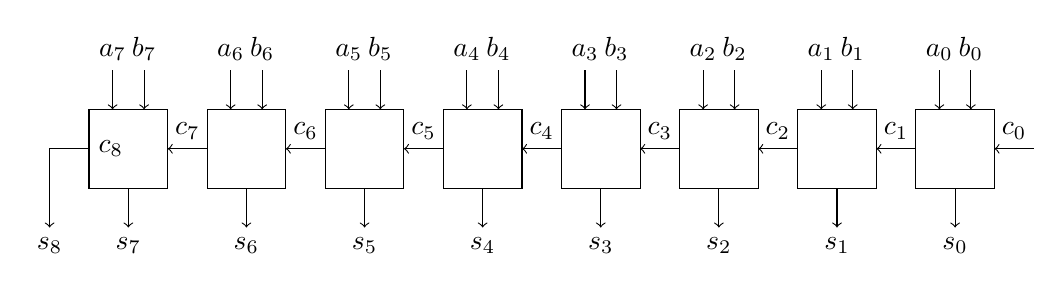
\begin{tikzpicture}[scale=0.5]
    \foreach \x [evaluate={\y=int(7-\x);\z=int(8-\x)}] in {0,1,...,7}
    {
        \draw (3*\x,0) rectangle (3*\x+2,2);
        \draw[->] (3*\x+1,0)  -- (3*\x+1,-1) node[anchor=north] {$s_\y$};
        \draw[->] (3*\x+3,1) -- node[midway,anchor=south] {$c_\y$} (3*\x+2,1);
        \draw[->] (3*\x+0.6,3) node[anchor=south] {$a_\y$} -- (3*\x+0.6,2) ;
        \draw[->] (3*\x+1.4,3) node[anchor=south] {$b_\y$} -- (3*\x+1.4,2) ;
    }
    \draw[->] (0,1) node[anchor=west] {$c_8$} -- (-1,1) -- (-1,-1) node[anchor=north] {$s_8$};
\end{tikzpicture}
}
\caption{}
\end{figure}

全加器接收三个输入$a,b,c_i$,其中$a,b$分别是两个加数,$c_i$是输入进位。全加器产生两个输出$s,c_o$,其中$s$是和,$c_o$是输出进位。全加器的真值表如\autoref{tab1819}。这个逻辑我们在\autoref{exa3}中已经讨论了。

\begin{table}[!ht]
\centering
\begin{tabular}{ccc|cc}
$a$&$b$&$c_i$&$c_o$&$s$\\\hline
0&0&0&0&0\\
0&0&1&0&1\\
0&1&0&0&1\\
0&1&1&1&0\\
1&0&0&0&1\\
1&0&1&1&0\\
1&1&0&1&0\\
1&1&1&1&1
\end{tabular}
\caption{全加器的真值表}\label{tab1819}
\end{table}

\begin{figure}[!ht]
\centering
\includegraphics{images/408.png}
\qquad
\includegraphics{images/409.png}
\caption{四位加法器。红线和蓝线分别表示两个加数,绿线为进位,黄线为和,底端绿线为溢出位。上面低位下面高位。}\label{fig37}
\end{figure}

有了全加器,直接把多个全加器首尾相连,就得到了一个加法器(\autoref{fig37})。这个加法器要求两个加数从低位到高位依次延迟一个逻辑帧输入。

\begin{figure}[!ht]
\centering
\includegraphics{images/410.png}
\qquad
\includegraphics{images/411.png}
\caption{四位累加器。两个加数依次输入红蓝线。上面低位下面高位。}\label{fig38}
\end{figure}

除了用组合逻辑,我们还可以用时序逻辑做加法器。降频电路有逢二进一的特性,所以可以直接用降频电路做一个加法器(\autoref{fig38})。与组合逻辑加法器不同,时序逻辑加法器实质上是累加器,如果不复位,那么每次输入都会直接累加到上一次的结果上。在时序逻辑加法器中,第二个加数各位要在同一个逻辑帧输入,或者低位延迟输入,这与组合逻辑加法器恰好相反。

在加法器上,时序逻辑的另一个优点是,把降频电路改成递次电路,就可以直接做任何进制的累加。\url{https://www.bilibili.com/video/av40474377/}中的进制转换实际上就是做了一个十进制累加器,每修改一个二进制数位就向累加器中加一个值或减一个值。

\subsection{减法器(Subtractor)}
有了补码这个工具,减法器和加法器就可以共用一个电路,我们只需要增加一些部件将其中一个加数取反加一。取反的操作是容易的,而加一的操作正好可以借用\autoref{tab1406}中我们没有用到的$c_0$。做出的组合逻辑加减法器如\autoref{fig39}所示,需要注意的是加法器的输入从低位到高位延迟一个逻辑帧,所以对每个数位取反的时候也要从低位到高位延迟一个逻辑帧,完成这项工作的是\autoref{fig39}中最右边一列逻辑门。

\begin{figure}[!ht]
\centering
\includegraphics{images/412.png}
\qquad
\includegraphics{images/413.png}
\caption{四位加减法器。顶端黄线控制加减法,0为加法,1为减法。计算加法时红线和蓝线分别表示两个加数。计算减法时蓝线为被减数,红线为减数。黄线为和,底端绿线为溢出位。上面低位下面高位。}\label{fig39}
\end{figure}

时序逻辑的减法器同样是使用补码运算,这里不给出具体实现。

\subsection{比较器(Comparator)}
比较两个数的大小,最简单的就是从高位向低位逐位比较。例如比较$a_{[7:0]}$和$b_{[7:0]}$两个8位二进制数,首先比较最高位$a_7$和$b_7$,如果它们相等再比较$a_6$和$b_6$,依此类推。最后我们可以得到一个逻辑表达式:
\[\begin{split}
a_{[7:0]}\mathtt{>}b_{[7:0]}=&(a_7\mathtt{>}b_7)(a_7\mathtt{==}b_7\& a_6\mathtt{>}b_6)(a_7\mathtt{==}b_7\& a_6\mathtt{==}b_6\& a_5\mathtt{>}b_5)\\
&(a_7\mathtt{==}b_7\& a_6\mathtt{==}b_6\& a_5\mathtt{==}b_5\& a_4\mathtt{>}b_4)\\
&(a_7\mathtt{==}b_7\& a_6\mathtt{==}b_6\& a_5\mathtt{==}b_5\& a_4\mathtt{==}b_4\& a_3\mathtt{>}b_3)\\
&(a_7\mathtt{==}b_7\& a_6\mathtt{==}b_6\& a_5\mathtt{==}b_5\& a_4\mathtt{==}b_4\& a_3\mathtt{==}b_3\& a_2\mathtt{>}b_2)\\
&(a_7\mathtt{==}b_7\& a_6\mathtt{==}b_6\& a_5\mathtt{==}b_5\& a_4\mathtt{==}b_4\& a_3\mathtt{==}b_3\& a_2\mathtt{==}b_2\& a_1\mathtt{>}b_1)\\
&(a_7\mathtt{==}b_7\& a_6\mathtt{==}b_6\& a_5\mathtt{==}b_5\& a_4\mathtt{==}b_4\& a_3\mathtt{==}b_3\& a_2\mathtt{==}b_2\& a_1\mathtt{==}b_1\& a_0\mathtt{>}b_0)
\end{split}\]
用\autoref{sec23}中的导出公式,我们得到了只包含初等布尔运算的逻辑表达式:
\[\begin{split}
a_{[7:0]}>b_{[7:0]}=&(a_7\&\textrm{\~{}}b_7)(\textrm{\~{}}a_7b_7\& a_6\&\textrm{\~{}}b_6)(\textrm{\~{}}a_7b_7\&\textrm{\~{}}a_6b_6\& a_5\&\textrm{\~{}}b_5)\\
					&(\textrm{\~{}}a_7b_7\&\textrm{\~{}}a_6b_6\&\textrm{\~{}}a_5b_5\& a_4\&\textrm{\~{}}b_4)\\
					&(\textrm{\~{}}a_7b_7\&\textrm{\~{}}a_6b_6\&\textrm{\~{}}a_5b_5\&\textrm{\~{}}a_4b_4\& a_3\&\textrm{\~{}}b_3)\\
					&(\textrm{\~{}}a_7b_7\&\textrm{\~{}}a_6b_6\&\textrm{\~{}}a_5b_5\&\textrm{\~{}}a_4b_4\&\textrm{\~{}}a_3b_3\& a_2\&\textrm{\~{}}b_2)\\
					&(\textrm{\~{}}a_7b_7\&\textrm{\~{}}a_6b_6\&\textrm{\~{}}a_5b_5\&\textrm{\~{}}a_4b_4\&\textrm{\~{}}a_3b_3\&\textrm{\~{}}a_2b_2\& a_1\&\textrm{\~{}}b_1)\\
					&(\textrm{\~{}}a_7b_7\&\textrm{\~{}}a_6b_6\&\textrm{\~{}}a_5b_5\&\textrm{\~{}}a_4b_4\&\textrm{\~{}}a_3b_3\&\textrm{\~{}}a_2b_2\&\textrm{\~{}}a_1b_1\& a_0\&\textrm{\~{}}b_0)
\end{split}\]

\begin{figure}
\centering
\includegraphics{images/396.png}\qquad\includegraphics{images/397.png}
\caption{逐位比较器。上方火把表示$b_{[7:0]}$,左边高位右边低位;右侧火把表示$a_{[7:0]}$,下方高位上方低位;左下火把表示$a_{[7:0]}\mathtt{>}b_{[7:0]}$。}\label{fig33}
\end{figure}
将这个逻辑表达式转换为电路如\autoref{fig33}所示。

比较两个数的大小,除了逐位比较之外,还可以直接将两个数做减法,并判断结果的正负性。减法器我们已经做过了,而补码表示中,一个数的正负可以直接通过最高位得出。这里有两个细节的问题。无符号整数没有符号位,如何比较两个无符号整数的大小?有符号整数的两数之差可以达到$127-(-128)=255=11111111$,而这个数作为有符号整数实际上表示$-1$,即小于0。如何处理这些特殊情况?事实上我们这里的比较器只能比较无符号整数,而所谓的“最高位”实际上指的是\autoref{tab1406}中的溢出位$s_8$。对于有符号整数有两种处理方法:第一种是首先判断符号,如果符号相等,再做无符号整数的比较;第二种是把两个数都加$128$,这样就把$-128\sim127$的范围变成了$0\sim255$,然后做无符号整数的比较即可。

比较两个数是否相等,也有两种解法,一种是直接逐位比较,另一种是判断它们的差是否为0。这两种方法并没有绝对的优劣,虽然逐位比较的电路会比较简单,但是判断差值的电路可以直接附加在其他功能上,例如加法器。

\subsection{乘法器(Multiplier)}
乘法是加法的推广,乘法器也是加法器的推广。我们首先来看二进制乘法的竖式计算。因为乘法规模较大,这里给出4位乘法的例子(\autoref{tab6585})。

\begin{figure}[!ht]
$$
\begin{array}{ccccccccc}
&&&&a_3&a_2&a_1&a_0\\
&&&&b_3&b_2&b_1&b_0\\\hline
&&&&b_0\&a_3&b_0\&a_2&b_0\&a_1&b_0\&a_0\\
&&&b_1\&a_3&b_1\&a_2&b_1\&a_1&b_1\&a_0\\
&&b_2\&a_3&b_2\&a_2&b_2\&a_1&b_2\&a_0\\
&b_3\&a_3&b_3\&a_2&b_3\&a_1&b_3\&a_0\\\hline
H_3&H_2&H_1&H_0&l_3&l_2&l_1&l_0
\end{array}
$$
\caption{乘法竖式计算}\label{tab6585}
\end{figure}

从\autoref{tab6585}可以看出来,做一个4位乘法实际上就是做4个数的加法。4个数的加法,可以按照运算顺序拆分成三次2个数的加法,如\autoref{fig79}所示。

\begin{figure}[!ht]
\centering
\begin{tikzpicture}
    \draw (0,0) rectangle node{加法器} (5,1);
    \draw (0,2) rectangle node{加法器} (5,3);
    \draw (0,4) rectangle node{加法器} (5,5);
    
    \draw[->] (2,6) node[anchor=south]{$a_1$} -- (2,5);
    \draw[->] (3,6) node[anchor=south]{$a_2$} -- (3,5);
    \draw[->] (2,4)  -- node[midway,anchor=east]{$a_1+a_2$} (2,3);
    \draw[->] (6,3.5) node[anchor=west]{$a_3$} -- (3,3.5) -- (3,3);
    \draw[->] (2,2)  -- node[midway,anchor=east]{$a_1+a_2+a_3$} (2,1);
    \draw[->] (6,1.5) node[anchor=west]{$a_4$} -- (3,1.5) -- (3,1);
    \draw[->] (2.5,0) -- (2.5,-1) node[anchor=north]{$a_1+a_2+a_3+a_4$};
\end{tikzpicture}
\caption{四个加数$a_1,a_2,a_3,a_4$连加}\label{fig79}
\end{figure}

把\autoref{fig79}中的加法器展开成串联的全加器,就得到了四位乘法器的结构示意图(\autoref{fig80})。

\begin{figure}[!ht]
\centering
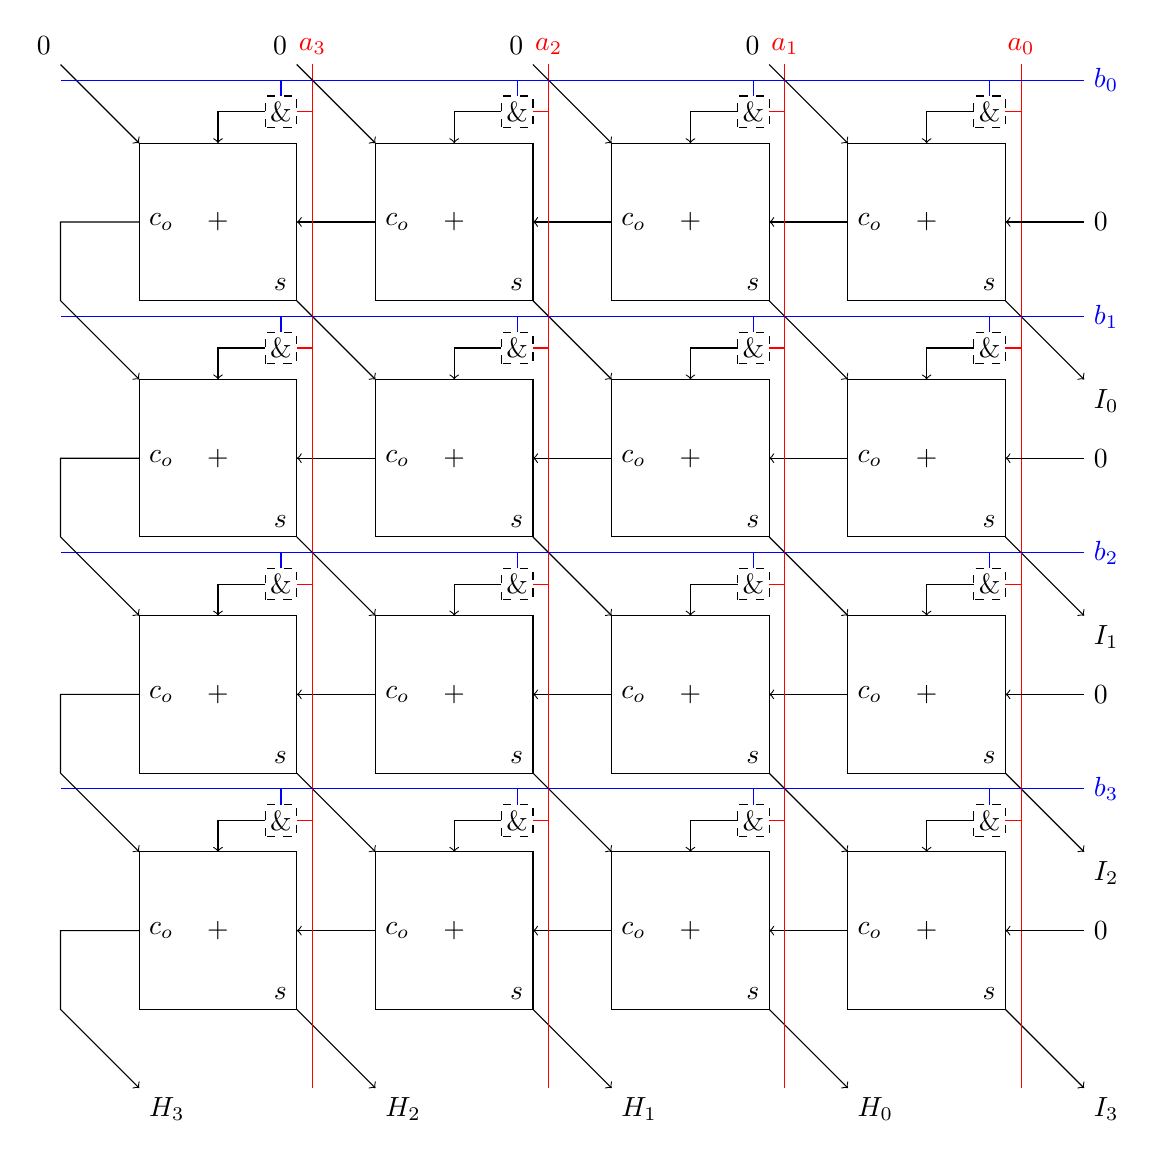
\begin{tikzpicture}
    \foreach \x [evaluate={\z=int(3-\x)}] in {0,1,2,3}
        \foreach \y [evaluate={\w=int(3-\y)}] in {0,1,2,3} {
            \draw (3*\x,3*\y) rectangle node {$+$} (3*\x+2,3*\y+2); % 全加器框架
            \draw[dashed] (3*\x+1.6,3*\y+2.2) rectangle node {\&} (3*\x+2,3*\y+2.6);
            \draw[->] (3*\x+1.6,3*\y+2.4) -- (3*\x+1,3*\y+2.4) -- (3*\x+1,3*\y+2);
            \draw[blue] (3*\x+1.8,3*\y+2.6) -- (3*\x+1.8,3*\y+2.8);
            \draw[red] (3*\x+2,3*\y+2.4) -- (3*\x+2.2,3*\y+2.4);
            \draw[->] (3*\x+2,3*\y) node[anchor=south east] {$s$} -- (3*\x+3,3*\y-1); % 和输出
        }
    \foreach \x in {1,2,3}
        \foreach \y in {0,1,2,3}
            \draw[->] (3*\x,3*\y+1) node[anchor=west] {$c_o$} -- (3*\x-1,3*\y+1); % 进位连接
    \foreach \x [evaluate={\z=int(3-\x)}] in {0,1,2,3}{
        \draw[->,] (3*\x-1,12) node[anchor=south east] {$0$} -- (3*\x,11); % 第一排缺省加数
        \draw (3*\x,-1) node[anchor=north west] {$H_\z$}; % 结果高四位
        \draw[red] (3*\x+2.2,12) node[anchor=south] {$a_\z$} -- (3*\x+2.2,-1); %乘数1输入
    }
    \foreach \y [evaluate={\w=int(3-\y)}] in {0,1,2,3}{
        \draw (12,3*\y-1) node[anchor=north west] {$I_\w$}; % 结果低四位
        \draw[->] (0,3*\y+1) node[anchor=west] {$c_o$} -- (-1,3*\y+1) -- (-1,3*\y) -- (0,3*\y-1); % 左边一列进位输出
        \draw[->] (12,3*\y+1) node[anchor=west] {$0$} -- (11,3*\y+1); % 右边一列进位输入
        \draw[blue] (12,3*\y+2.8) node[anchor=west] {$b_\w$}-- (-1,3*\y+2.8); % 乘数2输入
    }
\end{tikzpicture}
\caption{四位乘法器结构示意图。大的实线方框表示全加器,$c_o$表示进位输出,$s$表示和输出。小的虚线方框表示与门,红蓝线输入,黑线输出。两个乘数分别从上方和右方输入,乘积的低位从右边输出,高位从下边输出。全加器缺少的输入补零。左右相邻的两个全加器,右边的早一个逻辑帧;上下相邻的两个全加器,上边的早两个逻辑帧。}\label{fig80}
\end{figure}

乘法器的单个单元电路见\autoref{fig81},其中用不同颜色的背景墙标记区域和线路。橙色区域为全加器。黄色区域是与门。蓝色线路是从右边输入的乘数,每经过一个单元要延迟1个逻辑帧。红色线路是从上边输入的乘数,每经过一个单元要延迟2个逻辑帧。紫色线路是横向的进位传递。绿色线路是从左上到右下的和传递。

\begin{figure}[!ht]
\centering
\includegraphics{images/436.png}
\caption{乘法器单个单元的结构}\label{fig81}
\end{figure}

单元堆叠后的效果见\autoref{fig82},其中每个单元大小3*7。优化过程用到了如下的接线技巧:
\begin{itemize}
	\item 左右方向上红蓝线循环,便于接线。
	\item 相邻两列错位,便于进位和横向乘数的传递。
	\item 纵向的逻辑延迟用到了一个异或门,从而这个门不需要为经过的绿线让路。
	\item 与门利用了等式$a\&b=\textrm{\~{}} ab\&b$,便于接线。
\end{itemize}

\begin{figure}[!ht]
\centering
\includegraphics[width=\textwidth]{images/437.png}
\caption{堆叠优化后的效果}\label{fig82}
\end{figure}

\subsection{除法器(Divider)}
1
\subsection{移位器(Shifter)}
移位又分为逻辑移位、算术移位、循环移位,其中逻辑移位和算术移位应用较广。

\begin{figure}[!ht]
\centering
\subfloat[逻辑右移一位]{\includegraphics{images/414.png}}
\qquad
\subfloat[算术右移一位]{\includegraphics{images/415.png}}
\qquad
\subfloat[循环右移一位]{\includegraphics{images/416.png}}
\caption{递次电路移位}\label{fig40}
\end{figure}

如果只移一位的话,这三种移位都可以通过递次电路实现,如\autoref{fig40}所示。

\begin{figure}
\centering
\subfloat[逻辑右移]{\includegraphics[width=0.45\textwidth]{images/400.png}\qquad\includegraphics[width=0.45\textwidth]{images/401.png}}

\subfloat[算术右移]{\includegraphics[width=0.45\textwidth]{images/402.png}\qquad\includegraphics[width=0.45\textwidth]{images/403.png}}

\subfloat[经过简单优化的算术右移]{\includegraphics[width=0.45\textwidth]{images/404.png}\qquad\includegraphics[width=0.45\textwidth]{images/405.png}}
\caption{组合逻辑原理的移位器。右侧三个火把从上到下作用依次为移1位、移2位、移4位。}\label{fig35}
\end{figure}

如果要移任意位,递次电路大概率会爆门,此时需要考虑其他方案。一个简单的思路是使用\autoref{fig35}所示的组合逻辑。这个组合逻辑的缺点是,被移位数的所有数位输入要在同一个逻辑帧,而移位量的数位要在各个逻辑帧依次输入,调节逻辑同步较复杂。此外,由于逻辑门的取向问题,这种方法不适用于循环移位。

\begin{figure}[!ht]
\centering
\includegraphics{images/417.png}
\qquad
\includegraphics{images/418.png}
\caption{移位器。纵向的红蓝线输入待移位的数。横向红蓝线输入移位的位数。通过顶端的逻辑灯激活对应的输出。底端绿线用于切换逻辑移位和算术移位。}\label{fig41}
\end{figure}

事实上,因为数字电路结构都相对复杂,在泰拉瑞亚中想做一定规模的数字电路,一定要考虑利用\nameref{sec17}技术传输数据。\nameref{sec17}技术通过在不同逻辑帧发送不同数位传播数据,我们可以通过这一特点设计专门兼容\nameref{sec17}的移位器。\autoref{fig41}通过选取网线输出的起始数位实现移位功能。

\subsection{随机数生成器(Random Number Generator)}
在现实中需要用复杂算法实现的功能,在泰拉瑞亚中反而异常简单。直接使用8个1/2概率的故障逻辑门,我们就可以随机生成8位二进制数。
\vspace{5cm}

没了。

\subsection{进制转换}

\paragraph*{方法一} 直接用定义式$a_{n:0}=a_n2^n+a_{n-1}2^{n-1}+\cdots+a_02^0$。要利用这个式子将二进制转换为十进制,需要做一个十进制加法器,然后存储2的各次幂的十进制值。\url{https://www.bilibili.com/video/av40474377/}就是用的这种方法。

十进制转二进制可以用同样的原理,做一个二进制加法器,然后存储10的各次幂的二进制值。

\paragraph*{方法二} 利用\autoref{sec30}和\autoref{sec31}介绍的方法。在竖式的每一步中,我们需要做一个查表的操作,然后错一位。这个查表的操作实际上是一个组合逻辑,如\autoref{tab12}所示。

\begin{table}[!ht]
\centering
\begin{tabular}{|c|c|}
\hline
二进制&BCD\\\hline
0000&0000\\\hline
0001&0001\\\hline
0010&0010\\\hline
0011&0011\\\hline
0100&0100\\\hline
0101&1000\\\hline
0110&1001\\\hline
0111&1010\\\hline
1000&1011\\\hline
1001&1100\\\hline
\end{tabular}
\caption{二进制转BCD则从左到右查,BCD转二进制则从右到左查。}\label{tab12}
\end{table}

二进制转BCD和BCD转二进制对应不同的真值表,我们需要分开设计。

\section{存储电路}
一个存储电路总是要有一个用于存放数据的阵列和一个选择数据的多路选择器。

\subsection{多路选择器(Multiplexer)}
多路选择器接收一个二进制地址,激活该地址代表的位置。一个经典的四位多路选择器如\autoref{fig42}所示。

\begin{figure}[!ht]
\centering
\includegraphics{images/419.png}\vspace{16pt}

\includegraphics{images/420.png}
\caption{经典四位多路选择器。红蓝线表示地址,上面高位下面低位。绿线双激活输出。16个逻辑门从左到右依次表示0000到1111。}\label{fig42}
\end{figure}

我们在\nameref{sec2:2}中曾见过相似的电路,事实上那个就是状态版的多路选择器。本小节中我们通过\nameref{sec33}实现了激活版的多路选择器。

\subsection{只读存储器(Read-Only Memory)}
只读存储器用于存储事先设计好的、固定的数据。这些数据不需要在使用时修改,所以一般是通过物理方式直接做在电路中。
\begin{figure}[!ht]
    \centering
	\subfloat[横向输入纵向输出]{\label{fig49}\includegraphics{images/342.png}\quad\includegraphics{images/341.png}}
    \qquad
	\subfloat[纵向输入横向输出]{\label{fig50}\includegraphics{images/343.png}\quad\includegraphics{images/344.png}}
    \qquad
	\subfloat[纵向输入横向输出]{\label{fig51}\includegraphics{images/346.png}\quad\includegraphics{images/345.png}}
    \caption{ROM的三种设计。}\label{fig48}
\end{figure}
\autoref{fig48}展示了三种ROM设计。\autoref{fig49}使用故障逻辑灯存储数据。一根横线激活时,只有经过的故障逻辑灯下方的逻辑门才会激活。因为存储器要与多路选择器配合,而多路选择器是纵向输出,所以\autoref{fig49}目前没有实用价值。\autoref{fig50}和\autoref{fig51}都是通过接线存储数据,也是有广泛应用的两种ROM。两个电路在实现方式上的区别是,\autoref{fig50}通过连接输出线与逻辑门来存储,而\autoref{fig51}通过连接输入线与逻辑灯来存储。占用空间方面,\autoref{fig50}占用高度较低(1.5格/bit),\autoref{fig51}占用高度较高(2格/bit)。逻辑同步方面,\autoref{fig51}的输出是同步的,而\autoref{fig50}不同步,在本来就需要不同步的场景(例如很多\nameref{sec34}和\nameref{sec17}),\autoref{fig50}更好。

\nameref{sec2:2}中,\autoref{i36:37}就是状态式的多路选择器,\autoref{i42:43}的下半部分电路就是\autoref{fig50}样式的ROM。只有有限个输出情况的显示器都可以通过ROM实现。

\subsection{只写存储器(Write-Only Memory)}
1
\subsection{随机存储器(Random Access Memory)}
1
\subsection{寄存器(Register)}
1
\subsection{栈(Stack)}
1

\section{分段显示器化简理论}
1
\subsection{分段显示器主要结构}
1
\subsection{显示矩阵、分段矩阵和数字矩阵}
1
\subsection{矩阵的初等变换}
1
\subsection{化简原理与细节}
1

\section{处理器结构}
1
\subsection{汇编语言}
1
\subsection{机器语言}
1
\subsection{处理器的拓扑结构}
1
\subsection{数据路径(Data Path)}
1
\include{chapters/Sources}
%\include{chapters/chapter8}
\include{chapters/chapter5}
%\include{chapters/Farm}

%\nocite{*} 

%\bibliography{reference}

\appendix
\include{chapters/Furnitures}
\include{chapters/cooldown}
\include{chapters/knowledge}
\chapter{常用工具与网址}\label{app1}

\section{Wiki}\label{app2}
\href{https://terraria.gamepedia.com/Terraria_Wiki}{英文} | \href{https://terraria-zh.gamepedia.com/Terraria_Wiki}{中文} | \href{http://terraria.1tu.me/}{中文镜像站} | \href{http://trwiki.uu.cc/}{中文镜像(乐逗)} | \href{https://terraria-wiki.fileplanet.com/apk/download#}{英文apk}

\section{论坛}
\href{https://forums.terraria.org/index.php?forums/t-mec-terraria-mechanical-engineering-corps.194/}{官方论坛-[T-MEC]电路工程师联盟} | \href{https://github.com/putianyi889/TMECbackup}{T-MEC帖子存档} | \href{https://www.bbstr.net/}{中文论坛} | \href{https://www.curseforge.com/terraria/maps}{CurseForge地图下载}

\section{地图编辑器}\label{app3}
\href{https://github.com/TEdit/Terraria-Map-Editor}{主页} | \href{http://www.binaryconstruct.com/downloads/}{下载1} | \href{https://github.com/TEdit/Terraria-Map-Editor/releases}{下载2} | 推荐教程\href{http://v.youku.com/v_show/id_XMjYxNTUzOTMyOA}{(1)}\href{http://v.youku.com/v_show/id_XMjY0NDYwMTM3Ng}{(2)}\href{http://v.youku.com/v_show/id_XMjY1OTIzNjg4OA}{(3)}\href{http://v.youku.com/v_show/id_XMjY3ODQwODE1Ng}{(4)}

\section{模组}
\subsection{tModLoader}\label{app4}
\href{https://www.tmodloader.net/}{官网} | \href{https://github.com/tModLoader/tModLoader}{GitHub} | \href{https://github.com/tModLoader/tModLoader/releases}{下载} | \href{https://github.com/tModLoader/tModLoader/wiki}{Wiki} | \href{https://tmodloader.github.io/tModLoader/html/annotated.html}{文档}

\subsection{CheatSheet}\label{app5}
\href{https://github.com/JavidPack/CheatSheet}{主页} | \href{http://javid.ddns.net/tModLoader/download.php?Down=mods/CheatSheet.tmod}{下载1} | \href{https://github.com/JavidPack/CheatSheet/releases}{下载2} | \href{https://forums.terraria.org/index.php?threads/cheat-sheet.41407/}{发布页}

\subsection{HERO's Mod}\label{app6}
\href{https://github.com/JavidPack/HEROsMod}{主页} | \href{http://javid.ddns.net/tModLoader/download.php?Down=mods/HEROsMod.tmod}{下载1} | \href{https://github.com/JavidPack/HEROsMod/releases}{下载2} | \href{https://forums.terraria.org/index.php?threads/heros-mod-creative-mode-server-management-and-over-25-tools-1-3-4-4-compatible.44650/}{发布页}

\subsection{MechScope}\label{app7}
\href{https://github.com/DRKV333/MechScope}{主页} | \href{https://github.com/DRKV333/MechScope/releases/}{下载} | \href{https://forums.terraria.org/index.php?threads/mechscope-wiring-visualized.70665/}{发布页} | \href{https://www.bilibili.com/read/cv2222687}{中文介绍}

\section{源码}\label{app8}
\href{https://github.com/Pryaxis/Sources}{1.3.5及1.4各版本} | \href{https://github.com/NoviaDroid/TerrariaRefractoring_1.3.2.1}{1.3.2.1} | \href{https://github.com/saniainf/EDTerraria}{1.3} | \href{https://github.com/EdgeKiller/terrariaSource}{1.2.4.1} | \href{https://github.com/TheVamp/Terraria-Source-Code}{1.2.0.3.1} | \href{https://github.com/dptug/TerrariaXDK}{Xbox 360}

\chapter{推荐视频}
\section{教学}
\begin{itemize}
\item (Danger)泰拉瑞亚terraria 电路教学大全 \url{https://www.bilibili.com/video/av19065519}
\item 【Terraria】电路进阶(1) 电路结算与爆门 \url{https://www.bilibili.com/video/av56232462}
\item 【Terraria】电路进阶(2) 电路结算例子 \url{https://www.bilibili.com/video/av56612391}
\item 【Terraria】电路进阶(3) 等价逻辑 \url{https://www.bilibili.com/video/av56811001}
\item 【Terraria】电路进阶(4) 像素盒显示器 \url{https://www.bilibili.com/video/av57842510}
\item 泰拉瑞亚1.3pe高效率南瓜神教详细教程 \url{https://www.bilibili.com/video/av70594057}
\item 【Terraria】v1.0半自动与全自动树场建造(附全自动夜光蘑菇农场以及全自动仙人掌场地) \url{https://www.bilibili.com/video/av27408545}
\item 【Terraria电路】传送阵教学地图讲解 \url{https://www.bilibili.com/video/av24905110}
\item {[}Terraria]Mappygaming的视频粉丝问答 \url{https://www.bilibili.com/video/av22788696}
\item Terraria 旧日军团事件 Tips \& Tricks -MappyGaming \url{https://www.bilibili.com/video/av21707397}
\item {[}Terraria]鬼畜的石巨人!-Zerogravitas \url{https://www.bilibili.com/video/av22088547}
\item {[}Terraria]物品半砖以及一些有趣应用!-Zerogravitas \url{https://www.bilibili.com/video/av22739847}
\item \href{https://www.bilibili.com/video/BV1aa4y1t7VH?p=2}{硬上限原理简析及利用}
\end{itemize}

\section{视觉效果}
\begin{itemize}
\item Terraria Bad Apple!! \url{https://www.bilibili.com/video/av46694445}
\item 【泰拉瑞亚】彩虹小电视我们起飞 \url{https://www.bilibili.com/video/av16601896}
\item {[}Terraria]官方推荐电路作品-Bad apple(音乐为后期添加) \url{https://www.bilibili.com/video/av22343683}
\item 【Terraria电路】像素盒定格动画 兔子 \url{https://www.bilibili.com/video/av50343156}
\item {[}Terraria] Digi-Comp 2装置展示-Zerogravitas \url{https://www.bilibili.com/video/av22690346}
\item 泰拉瑞亚 有趣的矿车 \url{https://www.bilibili.com/video/av5271577}
\item 【Terraria电路】给女朋友的生日礼物 \url{https://www.bilibili.com/video/av21009075/}
\item Terraria in-game Pixel Art Animation \url{https://www.bilibili.com/video/av5301176/?p=5}
\item Terraria 莫尔条纹动画 兔子 \url{https://www.bilibili.com/video/av49966963}
\item Terraria 电子钟 \url{https://www.bilibili.com/video/av55613747}
\item Terraria 异世界四重奏 ED『異世界ガールズ・トーク』(传送器定格动画) \url{https://www.bilibili.com/video/av54977071}
\item \href{https://www.bilibili.com/video/BV1ME411P7QD}{泰 拉 复 印 机}
\end{itemize}

\section{小游戏}
\begin{itemize}
\item {[}Terraria]障碍挑战地图-Mappygaming \url{https://www.bilibili.com/video/av22787315}
\item 泰拉瑞亚 terraria 超难创意解谜地图通关介绍 (上) \url{https://www.bilibili.com/video/av19793617}
\item 泰拉瑞亚 terraria 超难创意解谜地图通关介绍 (中) \url{https://www.bilibili.com/video/av20101902}
\item 泰拉瑞亚 terraria 超难创意解谜地图通关介绍 (下) \url{https://www.bilibili.com/video/av20524074}
\item 泰拉瑞亚 在游戏里面玩游戏 \url{https://www.bilibili.com/video/av6594668}
\item {[}Terraria]使用传送枪达到最大速度!3000+mph! \url{https://www.bilibili.com/video/av24580434}
\item【Terraria】【FuryForged】冒险地图Harbinger通关实况 \url{https://www.bilibili.com/video/av37553671/}
\item 在Terraria中玩俄罗斯方块!? \url{https://www.bilibili.com/video/av38924330}
\item 在Terraria中解魔方? (Read Description) \url{https://www.bilibili.com/video/av56760618}
\item 泰拉瑞亚第一款五子棋 \url{https://www.bilibili.com/video/av93790872}
\item 【Terraria】生命游戏 \url{https://www.bilibili.com/video/av46416137}
\item 【Terraria】做贪吃蛇 \url{https://www.bilibili.com/video/av32265379}
\end{itemize}

\section{刷怪刷物品}
\begin{itemize}
\item {[}Terraria]半砖松露蠕虫农场(390+条/小时)!-DicemanX \url{https://www.bilibili.com/video/av23029412}
\item 泰拉瑞亚-诈个尸 \url{https://www.bilibili.com/video/av13411383}
\item 泰拉瑞亚 雕像回血裸装专家月总 \url{https://www.bilibili.com/video/av6393957}
\item 【Terraria电路】【Joe Price】全自动刷怪场、刷BOSS合集 专家模式 \url{https://www.bilibili.com/video/av32865707/}
\item Terraria 1.3.1 Pumpkin Moon Final Wave at 806 pm, 255 platinum coins in a night \url{https://www.bilibili.com/video/av5356226/?p=5}
\item Terraria 1.3 Frost Moon Final Wave at 856 pm, 75820 Total Points - World Record \url{https://www.bilibili.com/video/av5356226/?p=6}
\item 【泰拉瑞亚】最快的boss击杀集锦 无法被超越的世界纪录? \url{https://www.bilibili.com/video/av20725652}
\item 南瓜神教-旧日军团 \url{https://www.bilibili.com/video/av10885401/?p=3}
\item 南瓜神教-霜月夜 \url{https://www.bilibili.com/video/av10885401/?p=4}
\item 【Terraria电路】改进的高效全自动树场 \url{https://www.bilibili.com/video/av38882621/}
\item Terraria 刷石机 \url{https://www.bilibili.com/video/av50203346}
\item Terraria 水晶碎块农场 \url{https://www.bilibili.com/video/av57287619}
\end{itemize}

\chapter{推荐文献}

\section{机制研究}
\begin{itemize}
\item \href{https://www.bbstr.net/threads/469/}{【科普】松露人究竟需要什么?}
\item \href{https://www.bbstr.net/threads/463/}{【科普\&详解】为什么你的房子不合格?} 
\item \href{https://www.bbstr.net/threads/133/}{个人数字助手/手机显示的各种信息相关机制详解}
\item \href{https://www.bbstr.net/threads/lifesteal.198/}{【干货/灾厄/原版】LifeSteal—吸血冷却详解}
\item \href{https://www.bbstr.net/threads/tr.127/}{关于广播盒的各种应用技巧(TR字符串代码的应用)}
\item \href{https://www.bilibili.com/read/cv2156999}{【Terraria机制】傀儡教程}
\item 绳索glitch \href{https://forums.terraria.org/index.php?threads/someone-found-a-new-glitch.75822/}{Someone found a new glitch?}
\item 虚化家具glitch \href{https://forums.terraria.org/index.php?threads/actuating-tiles-using-sand.75811/}{Actuating tiles using sand}
\item 傀儡影子glitch \href{https://forums.terraria.org/index.php?threads/i-solved-the-rouge-dummy-glitch.76951/}{I solved the "Rouge Dummy" Glitch}
\item 烈焰机关 \href{https://forums.terraria.org/index.php?threads/flame-traps-and-teal-pads.76835/}{Flame Traps And Teal Pads}
\item 邪教徒AI \href{https://forums.terraria.org/index.php?threads/prototype-lunatic-cultist-farm-ai-analysis.77022/}{Prototype Lunatic Cultist Farm \& AI Analysis}
\end{itemize}

\section{半砖}
\begin{itemize}
\item 半砖驱动 \href{https://forums.terraria.org/index.php?threads/showcase-player-sensor-weighted-pressure-plate-engine.76597/}{[Showcase] Player Sensor/Weighted Pressure Plate Engine}
\item 半砖坐骑 \href{https://forums.terraria.org/index.php?threads/mount-hoik-tracks-and-teleportation.76953/}{Mount hoik tracks and teleportation}
\item 半砖史莱姆 \href{https://forums.terraria.org/index.php?threads/possible-to-hoik-slimes.75820/}{Possible to hoik slimes?}
\item 半砖城镇NPC \href{https://forums.terraria.org/index.php?threads/guide-using-character-npcs-in-hoiktronics-builds.75934/}{[Guide] Using Character NPCs in hoiktronics builds}
\item 半砖0帧换线器 \href{https://forums.terraria.org/index.php?threads/interesting-discovery-instant-one-way-signal-relay.77012/}{Interesting discovery: instant one way signal relay}
\item 用于传送机的半砖换线器/分线盒 \href{https://forums.terraria.org/index.php?threads/guide-bypassing-certain-colored-wires-with-teleporters.75929/}{[Guide] Bypassing certain colored wires with teleporters}
\item 半砖延迟 \href{https://forums.terraria.org/index.php?threads/guide-how-to-construct-switches-with-built-in-delays.75931/}{[Guide] How to construct switches with built-in delays}
\item 半砖竖直复位 \href{https://forums.terraria.org/index.php?threads/vertical-reset-mechanism.77035/}{Vertical reset mechanism}
\item 半砖随机数 \href{https://forums.terraria.org/index.php?threads/hoik-randomisers.77040/}{Hoik Randomisers}
\item 半砖传送阵 \href{https://forums.terraria.org/index.php?threads/guide-how-to-build-a-hoiktronics-based-teleporter-hub-updated-version.75867/}{[Guide] How to build a Hoiktronics-Based Teleporter Hub (updated version)}
\item 半砖传送阵改进 \href{https://forums.terraria.org/index.php?threads/diceman-teleporter-hub-tweaked.75979/}{Diceman Teleporter Hub Tweaked.}
\item 半砖密码门 \href{https://forums.terraria.org/index.php?threads/hoiktronics-programmable-passcode-protected-door-video-tutorial.12232/}{Hoiktronics: Programmable Passcode-Protected Door + Video Tutorial}
\item 半砖多位数显示 \href{https://forums.terraria.org/index.php?threads/project-displaying-multiple-digit-numbers-entered-in-sequence.75935/}{[Project] Displaying Multiple Digit Numbers Entered in Sequence}
\item 半砖栈式七段线十进制显示 \href{https://forums.terraria.org/index.php?threads/project-sequential-digit-input-machine-dummies-amazing-signaling-agents.75909/}{[Project] Sequential Digit Input Machine (dummies = amazing signaling agents)}
\item 基础半砖逻辑门 \href{https://forums.terraria.org/index.php?threads/guide-updated-universal-logic-gates.75913/}{[Guide] Updated Universal Logic Gates}
\item 定制半砖逻辑门 \href{https://forums.terraria.org/index.php?threads/guide-how-to-build-logic-gates-of-any-size-or-complexity.75911/}{[Guide] How to Build Logic Gates of Any Size or Complexity}
\item 通用半砖逻辑门 \href{https://forums.terraria.org/index.php?threads/project-universal-logic-gate-can-be-adapted-to-a-variety-of-functions-depending-on-wiring.75898/}{[Project] "Universal" Logic Gate (can be adapted to a variety of functions depending on wiring)}
\item 单帧半砖逻辑门 \href{https://forums.terraria.org/index.php?threads/guide-1-tick-logic-gates.77001/}{[Guide] 1 Tick Logic Gates}
\item 半砖逻辑模块 \href{https://forums.terraria.org/index.php?threads/mini-builds-small-mechanisms.76983/}{[Mini-Builds] Small Mechanisms}
\item 半砖组合逻辑 \href{https://forums.terraria.org/index.php?threads/video-tutorial-giant-hoiktronics-logic-gates.75904/}{[Video Tutorial] Giant Hoiktronics Logic Gates}
\item 半砖超前进位加法器 \href{https://forums.terraria.org/index.php?threads/digital-electronics-8-bit-ripple-carry-adder.77033/}{[Digital Electronics] 8-Bit Ripple-Carry Adder}
\item 半砖BCD转二进制 \href{https://forums.terraria.org/index.php?threads/project-bcd-to-binary-converter.75907/}{[Project] BCD-to-Binary Converter}
\item 半砖二进制转十进制 \href{https://forums.terraria.org/index.php?threads/video-guide-how-to-build-a-binary-to-decimal-converter.75926/}{[Video Guide] How to Build a Binary to Decimal Converter}
\item 半砖二-十进制转换 \href{https://forums.terraria.org/index.php?threads/project-binary-to-decimal-converter-double-dabble-method.75937/}{[Project] Binary to Decimal Converter (Double Dabble Method)}
\item 半砖十进制加法 \href{https://forums.terraria.org/index.php?threads/project-calculator-with-decimal-inputs-and-output-puzzling-issues-with-dummy-ghosts.75906/}{[Project] Calculator with Decimal Inputs and Output (puzzling issues with dummy ghosts)}
\item 半砖计算器 \href{https://forums.terraria.org/index.php?threads/video-guide-how-terraria-computers-function.75928/}{[Video Guide] How Terraria Computers function}
\item 人工智能雏形 \href{https://forums.terraria.org/index.php?threads/showcase-prototype-artificial-intelligence-inside-terraria-pre-1-3-1.75890/}{[Showcase] Prototype Artificial Intelligence inside Terraria (pre-1.3.1)}
\item 21点 \href{https://forums.terraria.org/index.php?threads/guide-hoiktronics-computer-programmed-to-play-blackjack-with-special-rules.75914/}{[Guide] Hoiktronics Computer Programmed to Play Blackjack (with special rules)}
\end{itemize}

\section{小型模块}
\begin{itemize}
\item 简单逻辑装置 \href{https://forums.terraria.org/index.php?threads/a-reference-guide-for-simple-logic-devices.81751/}{A reference guide for simple logic devices}
\item 飞镖机关枪 \href{https://forums.terraria.org/index.php?threads/tutorial-wip-cooldown-juggling-rapid-fire-dart-trap-engines-animated-guide.75871/}{[Tutorial WIP] Cooldown Juggling Rapid Fire Dart Trap Engines (Animated Guide)}
\item 液体彩色显示 \href{https://forums.terraria.org/index.php?threads/project-writing-in-neon.76053/}{[Project] Writing in Neon}
\item 掉落骗伤 \href{https://forums.terraria.org/index.php?threads/a-new-type-of-invulnerability-machine.76319/}{A new type of invulnerability machine}
\item 掉落骗伤 \href{https://forums.terraria.org/index.php?threads/fall-damage-prevention-for-lunar-pillar-event.76355/}{Fall Damage Prevention for Lunar Pillar Event}
\item 烟花盒驱动 \href{https://forums.terraria.org/index.php?threads/new-type-of-engine-fireworks.75788/}{New Type of Engine! Fireworks?}
\item 金币掉落装置 \href{https://forums.terraria.org/index.php?threads/showcase-reliable-coin-stack-breaker.75807/}{[showcase] Reliable coin stack breaker}
\item 机关钟表 \href{https://forums.terraria.org/index.php?threads/small-12-hour-clock.75810/}{Small (?) 12 hour clock!}
\item 恐惧驱动 \href{https://forums.terraria.org/index.php?threads/fear-engine.75835/}{Fear Engine}
\item 规避月总伤害 \href{https://forums.terraria.org/index.php?threads/moon-lord-damage-avoidance-tweak.75838/}{Moon Lord Damage Avoidance Tweak}
\item 用传送机做半砖循环 \href{https://forums.terraria.org/index.php?threads/a-hoik-loop-out-of-teleporters.75983/}{A hoik loop out of teleporters}
\item 传送带驱动 \href{https://forums.terraria.org/index.php?threads/ridiculously-small-player-above-sensor-engine.76326/}{Ridiculously Small Player Above Sensor Engine}
\item 门传送 \href{https://forums.terraria.org/index.php?threads/showcase-two-way-warp-chamber.76343/}{[Showcase] Two-Way Warp Chamber}
\item 使用异或门的ROM \href{https://forums.terraria.org/index.php?threads/perfect-3x5-4xn-pixel-display.76591/}{PERFECT 3x5 (4xN) pixel display!}
\item 液体计时 \href{https://forums.terraria.org/index.php?threads/liquid-trickle-timer-liquid-sensors-pumps-actuator.76803/}{Liquid Trickle Timer (Liquid Sensors, Pumps, Actuator)}
\item 液体复制 \href{https://forums.terraria.org/index.php?threads/project-showcase-more-efficient-liquid-duplication-flooding-the-world-in-survival.76943/}{[Project/Showcase] More efficient liquid duplication + flooding the world in survival}
\item 平台小技巧 \href{https://forums.terraria.org/index.php?threads/physics-ghost-town.76974/}{Physics. Ghost town.}
\item 开服传感器 \href{https://forums.terraria.org/index.php?threads/idea-device-world-load-detector.76984/}{[Idea/Device] World Load Detector}
\item 3*5显示 \href{https://forums.terraria.org/index.php?threads/project-unspaced-3-by-5-matrix-display.77062/}{[Project] unspaced, 3 by 5 matrix display}
\item 14段线和16段线字符显示 \href{https://forums.terraria.org/index.php?threads/project-14-and-16-segment-alphanumeric-displays.75927/}{[Project] 14 and 16 Segment Alphanumeric Displays}
\end{itemize}

\section{大型模块}
\begin{itemize}
\item 心雕阵(不用拾心药水)\href{https://forums.terraria.org/index.php?threads/showcase-the-fastest-possible-heart-generator-statue-farm.79848/}{[Showcase] The fastest possible heart generator (statue farm)}
\item 旋转锁 \href{https://forums.terraria.org/index.php?threads/showcase-reprogrammable-rotary-lock.75832/}{[Showcase] Reprogrammable rotary lock}
\item RAM \href{https://forums.terraria.org/index.php?threads/final-ram-design-and-update-on-the-computer-project.75973/}{Final RAM Design and Update on the Computer Project}
\item 滚动文字显示屏 \href{https://forums.terraria.org/index.php?threads/scrolling-text-on-a-programmable-text-board.76008/}{scrolling text on a programmable text board}
\item 硬盘 \href{https://forums.terraria.org/index.php?threads/compact-hard-drive.76091/}{Compact Hard Drive}
\item 像素盒显示器 \href{https://forums.terraria.org/index.php?threads/24-%C3%97-24-pixel-box-screen-w-16-configurable-animation-frames.76325/}{24 × 24 Pixel Box Screen w/16 Configurable Animation Frames}
\item 可编程密码锁 \href{https://forums.terraria.org/index.php?threads/project-reprogrammable-passcode-lock.76352/}{[Project] Reprogrammable passcode lock}
\item 铁轨逻辑 \href{https://forums.terraria.org/index.php?threads/tracktronics-how-to-build-a-computer-using-minecart-tracks.15202/}{Tracktronics: How to Build a Computer Using Minecart Tracks}
\item 服务器用密码门 \href{https://forums.terraria.org/index.php?threads/project-pvp-coded-door.77068/}{[Project] PvP Coded Door}
\end{itemize}

\section{电路作品}
\begin{itemize}
\item 海战小游戏 \href{https://forums.terraria.org/index.php?threads/real-working-battleship-minigame-with-logic-gates.85957/}{Real working battleship minigame with logic gates!}
\item 初等元胞自动机 \href{https://forums.terraria.org/index.php?threads/showcase-element-elementary-cellular-automaton.75798/}{[Showcase] elemenT - Elementary cellular automaton}
\item 16位计算机 \href{https://forums.terraria.org/index.php?threads/showcase-terrabyte-the-16-bit-programmable-computer.85479/}{[Showcase] TerraByte, the 16 Bit Programmable Computer}
\item 2D打印机 \href{https://forums.terraria.org/index.php?threads/showcase-2d-printer.75766/}{[Showcase] 2D Printer}
\item 打鸭子小游戏 \href{https://forums.terraria.org/index.php?threads/duck-duck-dart-duck-hunt-in-terraria.45200/}{Duck Duck Dart! (Duck Hunt in Terraria?)}
\item Nim小游戏 \href{https://forums.terraria.org/index.php?threads/nim-in-terraria.76089/}{Nim in Terraria}
\item \href{https://forums.terraria.org/index.php?threads/showcase-bad-apple.76348/}{[Showcase] Bad Apple!!}
\item 计算器 \href{https://forums.terraria.org/index.php?threads/showcase-a-calculator-using-only-logic-gates.76453/}{[Showcase] A calculator using only logic gates!}
\item 井字棋 \href{https://forums.terraria.org/index.php?threads/play-tic-tac-toe-in-terraria.76804/}{Play Tic Tac Toe in Terraria!}
\item 官方高尔夫地图 \href{https://forums.terraria.org/index.php?threads/terraria-journeys-end-official-golf-map-starter-kit.87208/}{Journey's End Official Golf Map Starter Kit}
\item 8位CPU \href{https://forums.terraria.org/index.php?threads/8-bit-cpu-v2-0.95542/}{8-bit CPU v2.0}
\end{itemize}

\section{建筑作品}
\begin{itemize}
\item 跑酷小游戏 \href{https://forums.terraria.org/index.php?threads/gotta-go-fast.63751/}{Gotta Go Fast!}
\item 大型建筑 \href{https://forums.terraria.org/index.php?threads/project-castlevania-sotn-a-to-scale-replica-of-draculas-castle.75802/}{[Project] Castlevania SOTN. A To-Scale Replica of Dracula's Castle.}
\item 大型建筑 \href{https://forums.terraria.org/index.php?threads/spaceship-hope-wiring.75855/}{Spaceship "HOPE" wiring}
\item 抽水马桶 \href{https://forums.terraria.org/index.php?threads/down-the-toilet.76349/}{Down the Toilet}
\item 官方解谜地图 \href{https://forums.terraria.org/index.php?threads/tales-of-the-terrarian.43625/}{Tales of the Terrarian}
	\begin{itemize}
	\item \href{https://forums.terraria.org/index.php?threads/how-its-made-tales-of-the-terrarian.76578/}{How It's Made: Tales of the Terrarian}
	\item \href{https://forums.terraria.org/index.php?threads/power-generator-tales-of-the-terrarian.76782/}{Power Generator - Tales of the Terrarian}
	\item \href{https://forums.terraria.org/index.php?threads/combining-player-sensors-tales-of-the-terrarian.76844/}{Combining Player Sensors - Tales of the Terrarian}
	\item \href{https://forums.terraria.org/index.php?threads/shooting-minigame-tales-of-the-terrarian.76842/}{Shooting Minigame - Tales of the Terrarian}
	\item \href{https://forums.terraria.org/index.php?threads/mechanical-boss-tales-of-the-terrarian.76742/}{Mechanical Boss - Tales of the Terrarian}
	\end{itemize}
\item 戈德堡机械 \href{https://forums.terraria.org/index.php?threads/rube-goldberg-machine.76620/}{Rube Goldberg Machine}
\end{itemize}

\section{农场}
\begin{itemize}
\item 全自动开荒 \href{https://forums.terraria.org/index.php?threads/mission-impossible-expert-mode-automated-playthrough-afk-from-pre-hardmode-to-moon-lord.75870/}{Mission Impossible: Expert Mode Automated Playthrough (AFK from Pre-Hardmode to Moon Lord)}
\item 采沙场 \href{https://forums.terraria.org/index.php?threads/automated-sand-factory-useless-farm.75846/}{Automated Sand Factory - Useless Farm?}
\item 松露虫农场 \href{https://forums.terraria.org/index.php?threads/showcase-truffle-worm-autofarm-390-worms-hr-50-plat-hr-bonus-best-way-to-farm-dev-armor.75848/}{[Showcase] Truffle Worm Autofarm: 390 Worms/hr + 50 Plat/hr (Bonus: Best Way to Farm Dev Armor)}
\item 月亮事件速杀场地 \href{https://forums.terraria.org/index.php?threads/showcase-lunar-event-speedrun-farm.76080/}{[Showcase] Lunar Event Speedrun Farm}
\item 改进的月亮事件速杀场地 \href{https://forums.terraria.org/index.php?threads/showcase-improved-lunar-event-speedkill-farm.75968/}{[Showcase] Improved Lunar Event Speedkill Farm}
\item 天梯神教 \href{https://forums.terraria.org/index.php?threads/showcase-1-3-pumpkin-frost-moon-new-records-arena.75976/}{[Showcase] 1.3 Pumpkin/Frost Moon New Records Arena}
\item 珊瑚农场 \href{https://forums.terraria.org/index.php?threads/super-compact-semi-automatic-coral-farm-buggy.76772/}{Super-Compact Semi-automatic coral farm [Buggy]}
\item 全自动地狱刷怪场(包括血肉墙) \href{https://forums.terraria.org/index.php?threads/showcase-recursive-wall-of-flesh-afk-autofarm-underworld-mob-grinder.75885/}{[Showcase] Recursive Wall of Flesh AFK Autofarm + Underworld Mob Grinder}
\item 蛛网农场 \href{https://forums.terraria.org/index.php?threads/automated-harvest-cobweb-farm.76865/}{Automated Harvest Cobweb Farm}
\item 同时与14个boss AFK战斗 \href{https://forums.terraria.org/index.php?threads/showcase-the-ultimate-battle-14-bosses-the-maximum-fought-simultaneously-afk-in-1-3-expert-mode.75897/}{[Showcase] The Ultimate Battle: 14 Bosses (the maximum) Fought Simultaneously AFK in 1.3 Expert Mode}
\item 全自动丛林刷怪场(包括世纪之花和石巨人) \href{https://forums.terraria.org/index.php?threads/showcase-expert-mode-temple-afk-autofarm-with-recursive-golem-and-plantera-autofarming.75900/}{[Showcase] Expert Mode Temple AFK Autofarm with Recursive Golem and Plantera Autofarming}
\item 全自动月亮事件 \href{https://forums.terraria.org/index.php?threads/project-expert-mode-recursive-fully-automated-lunar-event-autofarm.75902/}{[Project]Expert Mode Recursive Fully-Automated Lunar Event Autofarm}
\end{itemize}

\section{其他作品}
\begin{itemize}
\item 传送枪加速 \href{https://forums.terraria.org/index.php?threads/fastest-terrarian-ever-portal-gun-speed-boosts.76857/}{Fastest Terrarian ever! (portal gun speed boosts)}
\item 半砖脚本 \href{https://forums.terraria.org/index.php?threads/automating-the-construction-of-hoiks.76895/}{Automating the Construction of Hoiks}
\item 钓鱼脚本 \href{https://forums.terraria.org/index.php?threads/automating-fishing.76923/}{Automating Fishing}
\item 1.2之前的电路技术 \href{https://forums.terraria.org/index.php?threads/showcase-various-wiring-systems-in-custom-maps.77073/}{[Showcase] Various Wiring Systems in Custom Maps}
\end{itemize}

\chapter{人名代号}
这个附录中包含了本文档中提及的人名对应的论坛账号,以及本文档写作过程中参考过的作者及其贡献。如果这里漏掉了你的名字或者一些链接,欢迎至项目主页的Issues报告或直接通过Pull request提交修改。
\begin{itemize}
\item putianyi888:\href{https://space.bilibili.com/34937101}{bilibili} | \href{https://forums.terraria.org/index.php?members/putianyi888.121300/}{官方论坛} | \href{http://tieba.baidu.com/home/main?un=putianyi888}{百度贴吧} | \href{https://www.bbstr.net/members/putianyi888.342/}{中文论坛} | \href{https://www.youtube.com/channel/UCsG1EimffDYWXBoZRekcMIA}{YouTube} | \href{https://github.com/putianyi889}{GitHub}
\item usdanger:\href{https://space.bilibili.com/34637318/}{bilibili} | \href{http://i.youku.com/u/UMTcyMDA1MTY4}{优酷} | \href{http://tieba.baidu.com/home/main?un=us_danger}{百度贴吧} | \href{https://www.youtube.com/channel/UCh_cLX4iAbM6tAIl0zu3elw}{YouTube}
\item dcfhft:\href{https://space.bilibili.com/98605295/}{bilibili} | \href{http://tieba.baidu.com/home/main?un=dcfhft}{百度贴吧} | \href{https://www.bbstr.net/members/dcfhft.135/}{中文论坛}
\item 屠宰场:\href{https://space.bilibili.com/35610991/}{bilibili} | \href{https://www.bbstr.net/members/room.357/}{中文论坛}
\item 沉睡:\href{https://space.bilibili.com/22871583/}{bilibili}
\item 白霜心:\href{https://space.bilibili.com/49886444/}{bilibili} | \href{http://i.youku.com/u/UMTMyOTg1ODM4OA}{优酷} | \href{http://tieba.baidu.com/home/main?un=白霜心}{百度贴吧}
\item TNoName:\href{https://space.bilibili.com/14462041/}{bilibili} | \href{https://www.bbstr.net/members/tnoname.423/}{中文论坛}
\item 机锋哥:\href{http://i.youku.com/u/UMjg3MTI2NDcwOA}{优酷}
\item WIAADC:\href{https://space.bilibili.com/398780730}{bilibili} | \href{mailto:williamadcakc@outlook.com}{邮箱} | QQ:2607989335
\item ZeroGravitas:\href{https://forums.terraria.org/index.php?members/zerogravitas.96/}{官方论坛} | \href{https://www.youtube.com/channel/UCyLQbVwYleCYzgl49dNAeOw}{YouTube}
\item Programmatic:\href{https://forums.terraria.org/index.php?members/programmatic.37545/}{官方论坛} | \href{https://www.youtube.com/channel/UCWGTYKTR5Kw3cDhyd2vIDew}{YouTube}
\item TheRedStoneCrafter:\href{https://forums.terraria.org/index.php?members/idkwhoiam129.57457/}{官方论坛} | \href{https://www.youtube.com/channel/UC9ekQoOvO3BgFQsmGdWJpCQ}{YouTube}
\item ekinator:\href{https://forums.terraria.org/index.php?members/ekinator.61186/}{官方论坛}
\item DRKV:\href{https://forums.terraria.org/index.php?members/drkv.67603/}{官方论坛}
\item DicemanX:\href{https://forums.terraria.org/index.php?members/dicemanx.1706/}{官方论坛} | \href{https://www.youtube.com/channel/UCllYBm-_FbqWuI92o6zPXfw}{YouTube}
\item MappyGaming:\href{https://www.youtube.com/channel/UC-u6c7ppGML6icciJ0Q1oWQ}{YouTube}
\item KaiserYoshi:\href{https://forums.terraria.org/index.php?members/kaiseryoshi.680/}{官方论坛}
\end{itemize}

%\bibliography{reference}

\end{document}
%\end{lstlisting}


%\end{document}
